\documentclass{report}

%%%%%%%%%%%%%%%%%%%%%%%%%%%%%%%%%
% PACKAGE IMPORTS
%%%%%%%%%%%%%%%%%%%%%%%%%%%%%%%%%


% Codificación y tipografía básica (se cargan aquí para orden correcto)
\usepackage[utf8]{inputenc}
\usepackage[T1]{fontenc}
\usepackage{lmodern}
\usepackage{graphicx}
\usepackage{float}
\graphicspath{ {./Imagenes/} }
% Idioma español para nombres de elementos flotantes (Figura, Tabla, etc.)
% es-noindentfirst elimina la sangría automática tradicional del primer renglón tras títulos
\usepackage[spanish,es-noindentfirst]{babel}
% Asegurar nombre de tablas en español
\addto\captionsspanish{\renewcommand{\tablename}{Tabla}}
\usepackage[tmargin=2cm,rmargin=1in,lmargin=1in,margin=0.85in,bmargin=2cm,footskip=.2in]{geometry}
\usepackage{amsmath,amsfonts,amsthm,amssymb,mathtools}
\usepackage[varbb]{newpxmath}
\usepackage{xfrac}
\usepackage[makeroom]{cancel}
\usepackage{mathtools}
\usepackage{bookmark}
\usepackage{enumitem}
\usepackage{hyperref,theoremref}
\hypersetup{
    pdftitle={Assignment},
    colorlinks=true, linkcolor=gray,citecolor=blue,
    bookmarksnumbered=true,
    bookmarksopen=true
}
\usepackage[most,many,breakable]{tcolorbox}
\usepackage{xcolor}
\usepackage{colortbl}
\usepackage{varwidth}
\usepackage{varwidth}
\usepackage{etoolbox}
%\usepackage{authblk}
\usepackage{nameref}
\usepackage{multicol,array}
\usepackage{tikz-cd}
\usepackage[ruled,vlined,linesnumbered]{algorithm2e}
\usepackage{comment} % enables the use of multi-line comments (\ifx \fi) 
\usepackage{import}
\usepackage{xifthen}
\usepackage{pdfpages}
\usepackage{transparent}

\newcommand\mycommfont[1]{\footnotesize\ttfamily\textcolor{blue}{#1}}
\SetCommentSty{mycommfont}
\newcommand{\incfig}[1]{%
    \def\svgwidth{\columnwidth}
    \import{./figures/}{#1.pdf_tex}
}

\usepackage{tikzsymbols}
\renewcommand\qedsymbol{$\Laughey$}


%\usepackage{import}
%\usepackage{xifthen}
%\usepackage{pdfpages}
%\usepackage{transparent}


%%%%%%%%%%%%%%%%%%%%%%%%%%%%%%
% SELF MADE COLORS
%%%%%%%%%%%%%%%%%%%%%%%%%%%%%%



\definecolor{myg}{RGB}{56, 140, 70}
\definecolor{myb}{RGB}{45, 111, 177}
\definecolor{myr}{RGB}{199, 68, 64}
\definecolor{mytheorembg}{HTML}{F2F2F9}
\definecolor{mytheoremfr}{HTML}{00007B}
\definecolor{mylenmabg}{HTML}{FFFAF8}
\definecolor{mylenmafr}{HTML}{983b0f}
\definecolor{mypropbg}{HTML}{f2fbfc}
\definecolor{mypropfr}{HTML}{191971}
\definecolor{myexamplebg}{HTML}{F2FBF8}
\definecolor{myexamplefr}{HTML}{88D6D1}
\definecolor{myexampleti}{HTML}{2A7F7F}
\definecolor{mydefinitbg}{HTML}{E5E5FF}
\definecolor{mydefinitfr}{HTML}{3F3FA3}
\definecolor{notesgreen}{RGB}{0,162,0}
\definecolor{myp}{RGB}{197, 92, 212}
\definecolor{mygr}{HTML}{2C3338}
\definecolor{myred}{RGB}{127,0,0}
\definecolor{myyellow}{RGB}{169,121,69}
\definecolor{myexercisebg}{HTML}{F2FBF8}
\definecolor{myexercisefg}{HTML}{88D6D1}
\definecolor{mylightbrown}{HTML}{C4A484}


%%%%%%%%%%%%%%%%%%%%%%%%%%%%
% TCOLORBOX SETUPS
%%%%%%%%%%%%%%%%%%%%%%%%%%%%

\setlength{\parindent}{0pt}
\raggedright

%================================
% THEOREM BOX
%================================

\tcbuselibrary{theorems,skins,hooks}
\newtcbtheorem[number within=section]{Theorem}{Theorem}
{%
    enhanced,
    breakable,
    colback = mytheorembg,
    frame hidden,
    boxrule = 0sp,
    borderline west = {2pt}{0pt}{mytheoremfr},
    sharp corners,
    detach title,
    before upper = \tcbtitle\par\smallskip,
    coltitle = mytheoremfr,
    fonttitle = \bfseries\sffamily,
    description font = \mdseries,
    separator sign none,
    segmentation style={solid, mytheoremfr},
}
{th}

\tcbuselibrary{theorems,skins,hooks}
\newtcbtheorem[number within=chapter]{theorem}{Theorem}
{%
    enhanced,
    breakable,
    colback = mytheorembg,
    frame hidden,
    boxrule = 0sp,
    borderline west = {2pt}{0pt}{mytheoremfr},
    sharp corners,
    detach title,
    before upper = \tcbtitle\par\smallskip,
    coltitle = mytheoremfr,
    fonttitle = \bfseries\sffamily,
    description font = \mdseries,
    separator sign none,
    segmentation style={solid, mytheoremfr},
}
{th}


\tcbuselibrary{theorems,skins,hooks}
\newtcolorbox{Theoremcon}
{%
    enhanced
    ,breakable
    ,colback = mytheorembg
    ,frame hidden
    ,boxrule = 0sp
    ,borderline west = {2pt}{0pt}{mytheoremfr}
    ,sharp corners
    ,description font = \mdseries
    ,separator sign none
}

%================================
% Corolario e Importante
%================================
\tcbuselibrary{theorems,skins,hooks}
\newtcbtheorem[number within=section]{Corolario}{Corolario}
{%
    enhanced
    ,breakable
    ,colback = myp!10
    ,frame hidden
    ,boxrule = 0sp
    ,borderline west = {2pt}{0pt}{myp!85!black}
    ,sharp corners
    ,detach title
    ,before upper = \tcbtitle\par\smallskip
    ,coltitle = myp!85!black
    ,fonttitle = \bfseries\sffamily
    ,description font = \mdseries
    ,separator sign none
    ,segmentation style={solid, myp!85!black}
}
{th}
\tcbuselibrary{theorems,skins,hooks}
\newtcbtheorem[number within=chapter]{corolario}{Corolario}
{%
    enhanced
    ,breakable
    ,colback = myp!10
    ,frame hidden
    ,boxrule = 0sp
    ,borderline west = {2pt}{0pt}{myp!85!black}
    ,sharp corners
    ,detach title
    ,before upper = \tcbtitle\par\smallskip
    ,coltitle = myp!85!black
    ,fonttitle = \bfseries\sffamily
    ,description font = \mdseries
    ,separator sign none
    ,segmentation style={solid, myp!85!black}
}
{th}

\newtcolorbox{ImportanteBox}[1][]{%
    enhanced
    ,breakable
    ,colback = myp!10
    ,frame hidden
    ,boxrule = 0sp
    ,borderline west = {2pt}{0pt}{myp!85!black}
    ,sharp corners
    ,detach title
    ,before upper = \tcbtitle\par\smallskip
    ,coltitle = myp!85!black
    ,fonttitle = \bfseries\sffamily
    ,description font = \mdseries
    ,title = ¡IMPORTANTE!
    ,#1
}


%================================
% LENMA
%================================

\tcbuselibrary{theorems,skins,hooks}
\newtcbtheorem[number within=section]{Lenma}{Lenma}
{%
    enhanced,
    breakable,
    colback = mylenmabg,
    frame hidden,
    boxrule = 0sp,
    borderline west = {2pt}{0pt}{mylenmafr},
    sharp corners,
    detach title,
    before upper = \tcbtitle\par\smallskip,
    coltitle = mylenmafr,
    fonttitle = \bfseries\sffamily,
    description font = \mdseries,
    separator sign none,
    segmentation style={solid, mylenmafr},
}
{th}

\tcbuselibrary{theorems,skins,hooks}
\newtcbtheorem[number within=chapter]{lenma}{Lenma}
{%
    enhanced,
    breakable,
    colback = mylenmabg,
    frame hidden,
    boxrule = 0sp,
    borderline west = {2pt}{0pt}{mylenmafr},
    sharp corners,
    detach title,
    before upper = \tcbtitle\par\smallskip,
    coltitle = mylenmafr,
    fonttitle = \bfseries\sffamily,
    description font = \mdseries,
    separator sign none,
    segmentation style={solid, mylenmafr},
}
{th}


%================================
% PROPOSITION
%================================

\tcbuselibrary{theorems,skins,hooks}
\newtcbtheorem[number within=section]{Prop}{Proposition}
{%
    enhanced,
    breakable,
    colback = mypropbg,
    frame hidden,
    boxrule = 0sp,
    borderline west = {2pt}{0pt}{mypropfr},
    sharp corners,
    detach title,
    before upper = \tcbtitle\par\smallskip,
    coltitle = mypropfr,
    fonttitle = \bfseries\sffamily,
    description font = \mdseries,
    separator sign none,
    segmentation style={solid, mypropfr},
}
{th}

\tcbuselibrary{theorems,skins,hooks}
\newtcbtheorem[number within=chapter]{prop}{Proposition}
{%
    enhanced,
    breakable,
    colback = mypropbg,
    frame hidden,
    boxrule = 0sp,
    borderline west = {2pt}{0pt}{mypropfr},
    sharp corners,
    detach title,
    before upper = \tcbtitle\par\smallskip,
    coltitle = mypropfr,
    fonttitle = \bfseries\sffamily,
    description font = \mdseries,
    separator sign none,
    segmentation style={solid, mypropfr},
}
{th}


%================================
% CLAIM
%================================

\tcbuselibrary{theorems,skins,hooks}
\newtcbtheorem[number within=section]{claim}{Claim}
{%
    enhanced
    ,breakable
    ,colback = myg!10
    ,frame hidden
    ,boxrule = 0sp
    ,borderline west = {2pt}{0pt}{myg}
    ,sharp corners
    ,detach title
    ,before upper = \tcbtitle\par\smallskip
    ,coltitle = myg!85!black
    ,fonttitle = \bfseries\sffamily
    ,description font = \mdseries
    ,separator sign none
    ,segmentation style={solid, myg!85!black}
}
{th}



%================================
% Exercise
%================================

\tcbuselibrary{theorems,skins,hooks}
\newtcbtheorem[number within=section]{Exercise}{Exercise}
{%
    enhanced,
    breakable,
    colback = myexercisebg,
    frame hidden,
    boxrule = 0sp,
    borderline west = {2pt}{0pt}{myexercisefg},
    sharp corners,
    detach title,
    before upper = \tcbtitle\par\smallskip,
    coltitle = myexercisefg,
    fonttitle = \bfseries\sffamily,
    description font = \mdseries,
    separator sign none,
    segmentation style={solid, myexercisefg},
}
{th}

\tcbuselibrary{theorems,skins,hooks}
\newtcbtheorem[number within=chapter]{exercise}{Exercise}
{%
    enhanced,
    breakable,
    colback = myexercisebg,
    frame hidden,
    boxrule = 0sp,
    borderline west = {2pt}{0pt}{myexercisefg},
    sharp corners,
    detach title,
    before upper = \tcbtitle\par\smallskip,
    coltitle = myexercisefg,
    fonttitle = \bfseries\sffamily,
    description font = \mdseries,
    separator sign none,
    segmentation style={solid, myexercisefg},
}
{th}

%================================
% EXAMPLE BOX
%================================

\newtcbtheorem[number within=section]{Example}{Ejemplo}
{%
    colback = myexamplebg
    ,breakable
    ,colframe = myexamplefr
    ,coltitle = myexampleti
    ,boxrule = 1pt
    ,sharp corners
    ,detach title
    ,before upper=\tcbtitle\par\smallskip
    ,fonttitle = \bfseries
    ,description font = \mdseries
    ,separator sign none
    ,description delimiters parenthesis
}
{ex}

\newtcbtheorem[number within=chapter]{example}{Ejemplo}
{%
    colback = myexamplebg
    ,breakable
    ,colframe = myexamplefr
    ,coltitle = myexampleti
    ,boxrule = 1pt
    ,sharp corners
    ,detach title
    ,before upper=\tcbtitle\par\smallskip
    ,fonttitle = \bfseries
    ,description font = \mdseries
    ,separator sign none
    ,description delimiters parenthesis
}
{ex}

%================================
% DEFINITION BOX
%================================

\newtcbtheorem[number within=section]{Definición}{Definición}{enhanced,
    before skip=2mm,after skip=2mm, colback=red!5,colframe=red!80!black,boxrule=0.5mm,
    attach boxed title to top left={xshift=1cm,yshift*=1mm-\tcboxedtitleheight}, varwidth boxed title*=-3cm,
    boxed title style={frame code={
                    \path[fill=tcbcolback]
                    ([yshift=-1mm,xshift=-1mm]frame.north west)
                    arc[start angle=0,end angle=180,radius=1mm]
                    ([yshift=-1mm,xshift=1mm]frame.north east)
                    arc[start angle=180,end angle=0,radius=1mm];
                    \path[left color=tcbcolback!60!black,right color=tcbcolback!60!black,
                        middle color=tcbcolback!80!black]
                    ([xshift=-2mm]frame.north west) -- ([xshift=2mm]frame.north east)
                    [rounded corners=1mm]-- ([xshift=1mm,yshift=-1mm]frame.north east)
                    -- (frame.south east) -- (frame.south west)
                    -- ([xshift=-1mm,yshift=-1mm]frame.north west)
                    [sharp corners]-- cycle;
                },interior engine=empty,
        },
    fonttitle=\bfseries,
    title={#2},#1}{def}
\newtcbtheorem[number within=chapter]{definición}{Definición}{enhanced,
    before skip=2mm,after skip=2mm, colback=red!5,colframe=red!80!black,boxrule=0.5mm,
    attach boxed title to top left={xshift=1cm,yshift*=1mm-\tcboxedtitleheight}, varwidth boxed title*=-3cm,
    boxed title style={frame code={
                    \path[fill=tcbcolback]
                    ([yshift=-1mm,xshift=-1mm]frame.north west)
                    arc[start angle=0,end angle=180,radius=1mm]
                    ([yshift=-1mm,xshift=1mm]frame.north east)
                    arc[start angle=180,end angle=0,radius=1mm];
                    \path[left color=tcbcolback!60!black,right color=tcbcolback!60!black,
                        middle color=tcbcolback!80!black]
                    ([xshift=-2mm]frame.north west) -- ([xshift=2mm]frame.north east)
                    [rounded corners=1mm]-- ([xshift=1mm,yshift=-1mm]frame.north east)
                    -- (frame.south east) -- (frame.south west)
                    -- ([xshift=-1mm,yshift=-1mm]frame.north west)
                    [sharp corners]-- cycle;
                },interior engine=empty,
        },
    fonttitle=\bfseries,
    title={#2},#1}{def}



%================================
% Solution BOX
%================================

\makeatletter
\newtcbtheorem{question}{Pregunta}{enhanced,
    breakable,
    colback=white,
    colframe=myb!80!black,
    attach boxed title to top left={yshift*=-\tcboxedtitleheight},
    fonttitle=\bfseries,
    title={#2},
    boxed title size=title,
    boxed title style={%
            sharp corners,
            rounded corners=northwest,
            colback=tcbcolframe,
            boxrule=0pt,
        },
    underlay boxed title={%
            \path[fill=tcbcolframe] (title.south west)--(title.south east)
            to[out=0, in=180] ([xshift=5mm]title.east)--
            (title.center-|frame.east)
            [rounded corners=\kvtcb@arc] |-
            (frame.north) -| cycle;
        },
    #1
}{def}
\makeatother

%================================
% SOLUTION BOX
%================================

\makeatletter
\newtcolorbox{solution}{enhanced,
    breakable,
    colback=white,
    colframe=myg!80!black,
    attach boxed title to top left={yshift*=-\tcboxedtitleheight},
    title=Solution,
    boxed title size=title,
    boxed title style={%
            sharp corners,
            rounded corners=northwest,
            colback=tcbcolframe,
            boxrule=0pt,
        },
    underlay boxed title={%
            \path[fill=tcbcolframe] (title.south west)--(title.south east)
            to[out=0, in=180] ([xshift=5mm]title.east)--
            (title.center-|frame.east)
            [rounded corners=\kvtcb@arc] |-
            (frame.north) -| cycle;
        },
}
\makeatother

%================================
% Prueba de Clase BOX
%================================

\makeatletter
\newtcbtheorem{prueba}{Prueba de clase}{enhanced,
    breakable,
    colback=white,
    colframe=mylightbrown!90!black,
    attach boxed title to top left={yshift*=-\tcboxedtitleheight},
    fonttitle=\bfseries,
    title={#2},
    boxed title size=title,
    boxed title style={%
            sharp corners,
            rounded corners=northwest,
            colback=tcbcolframe,
            boxrule=0pt,
        },
    underlay boxed title={%
            \path[fill=tcbcolframe] (title.south west)--(title.south east)
            to[out=0, in=180] ([xshift=5mm]title.east)--
            (title.center-|frame.east)
            [rounded corners=\kvtcb@arc] |-
            (frame.north) -| cycle;
        },
    #1
}{prb}
\makeatother

%================================
% Question BOX
%================================

\makeatletter
\newtcbtheorem{qstion}{Pregunta}{enhanced,
    breakable,
    colback=white,
    colframe=mygr,
    attach boxed title to top left={yshift*=-\tcboxedtitleheight},
    fonttitle=\bfseries,
    title={#2},
    boxed title size=title,
    boxed title style={%
            sharp corners,
            rounded corners=northwest,
            colback=tcbcolframe,
            boxrule=0pt,
        },
    underlay boxed title={%
            \path[fill=tcbcolframe] (title.south west)--(title.south east)
            to[out=0, in=180] ([xshift=5mm]title.east)--
            (title.center-|frame.east)
            [rounded corners=\kvtcb@arc] |-
            (frame.north) -| cycle;
        },
    #1
}{def}
\makeatother

\newtcbtheorem[number within=chapter]{wconc}{Wrong Concept}{
    breakable,
    enhanced,
    colback=white,
    colframe=myr,
    arc=0pt,
    outer arc=0pt,
    fonttitle=\bfseries\sffamily\large,
    colbacktitle=myr,
    attach boxed title to top left={},
    boxed title style={
            enhanced,
            skin=enhancedfirst jigsaw,
            arc=3pt,
            bottom=0pt,
            interior style={fill=myr}
        },
    #1
}{def}



%================================
% NOTE BOX
%================================

\usetikzlibrary{arrows,calc,shadows.blur,shapes.geometric,mindmap,intersections,patterns}
\tcbuselibrary{skins}
\newtcolorbox{note}[1][]{%
    enhanced jigsaw,
    colback=gray!20!white,%
    colframe=gray!80!black,
    size=small,
    boxrule=1pt,
    title=\textbf{Nota:},
    halign title=flush center,
    coltitle=black,
    breakable,
    drop shadow=black!50!white,
    attach boxed title to top left={xshift=1cm,yshift=-\tcboxedtitleheight/2,yshifttext=-\tcboxedtitleheight/2},
    minipage boxed title=1.5cm,
    boxed title style={%
            colback=white,
            size=fbox,
            boxrule=1pt,
            boxsep=2pt,
            underlay={%
                    \coordinate (dotA) at ($(interior.west) + (-0.5pt,0)$);
                    \coordinate (dotB) at ($(interior.east) + (0.5pt,0)$);
                    \begin{scope}
                        \clip (interior.north west) rectangle ([xshift=3ex]interior.east);
                        \filldraw [white, blur shadow={shadow opacity=60, shadow yshift=-.75ex}, rounded corners=2pt] (interior.north west) rectangle (interior.south east);
                    \end{scope}
                    \begin{scope}[gray!80!black]
                        \fill (dotA) circle (2pt);
                        \fill (dotB) circle (2pt);
                    \end{scope}
                },
        },
    #1,
}

%%%%%%%%%%%%%%%%%%%%%%%%%%%%%%
% SELF MADE COMMANDS
%%%%%%%%%%%%%%%%%%%%%%%%%%%%%%


\newcommand{\thm}[2]{\begin{Theorem}{#1}{}#2\end{Theorem}}
\newcommand{\cor}[2]{\begin{Corolario}{#1}{}#2\end{Corolario}}
\newcommand{\imp}[1]{\begin{ImportanteBox}#1\end{ImportanteBox}}
\newcommand{\mlenma}[2]{\begin{Lenma}{#1}{}#2\end{Lenma}}
\newcommand{\mprop}[2]{\begin{Prop}{#1}{}#2\end{Prop}}
\newcommand{\clm}[3]{\begin{claim}{#1}{#2}#3\end{claim}}
\newcommand{\wc}[2]{\begin{wconc}{#1}{}\setlength{\parindent}{1cm}#2\end{wconc}}
\newcommand{\thmcon}[1]{\begin{Theoremcon}{#1}\end{Theoremcon}}
\newcommand{\ex}[2]{\begin{Example}{#1}{}#2\end{Example}}
\newcommand{\dfn}[2]{\begin{Definición}[colbacktitle=red!75!black]{#1}{}#2\end{Definición}}
\newcommand{\dfnc}[2]{\begin{Definición}[colbacktitle=red!75!black]{#1}{}#2\end{Definición}}
\newcommand{\qs}[2]{\begin{question}{#1}{}#2\end{question}}
\newcommand{\pf}[2]{\begin{myproof}[#1]#2\end{myproof}}
\newtcolorbox{comprobacion}[1][]{%
    enhanced jigsaw,
    colback=brown!12!white,%
    colframe=brown!75!black,
    size=small,
    boxrule=1pt,
    title=\textbf{Comprobación:},
    halign title=flush center,
    coltitle=black,
    breakable,
    drop shadow=black!40!white,
    attach boxed title to top left={xshift=1cm,yshift=-\tcboxedtitleheight/2,yshifttext=-\tcboxedtitleheight/2},
    minipage boxed title=2.8cm,
    boxed title style={%
            colback=white,
            size=fbox,
            boxrule=1pt,
            boxsep=2pt,
            underlay={%
                    \coordinate (dotA) at ($(interior.west) + (-0.5pt,0)$);
                    \coordinate (dotB) at ($(interior.east) + (0.5pt,0)$);
                    \begin{scope}
                        \clip (interior.north west) rectangle ([xshift=3ex]interior.east);
                        \filldraw [white, blur shadow={shadow opacity=60, shadow yshift=-.75ex}, rounded corners=2pt] (interior.north west) rectangle (interior.south east);
                    \end{scope}
                    \begin{scope}[brown!75!black]
                        \fill (dotA) circle (2pt);
                        \fill (dotB) circle (2pt);
                    \end{scope}
                },
        },
    #1,
}

\newcommand{\nt}[1]{\begin{note}#1\end{note}}
\newcommand{\comp}[1]{\begin{comprobacion}#1\end{comprobacion}}

\newcommand*\circled[1]{\tikz[baseline=(char.base)]{
        \node[shape=circle,draw,inner sep=1pt] (char) {#1};}}
\newcommand\getcurrentref[1]{%
    \ifnumequal{\value{#1}}{0}
    {??}
    {\the\value{#1}}%
}
\newcommand{\getCurrentSectionNumber}{\getcurrentref{section}}
\newenvironment{myproof}[1][\proofname]{%
    \proof[\bfseries #1: ]%
}{\endproof}

\newcommand{\mclm}[2]{\begin{myclaim}[#1]#2\end{myclaim}}
\newenvironment{myclaim}[1][\claimname]{\proof[\bfseries #1: ]}{}

\newcounter{mylabelcounter}

\makeatletter
\newcommand{\setword}[2]{%
    \phantomsection
    #1\def\@currentlabel{\unexpanded{#1}}\label{#2}%
}
\makeatother




\tikzset{
    symbol/.style={
            draw=none,
            every to/.append style={
                    edge node={node [sloped, allow upside down, auto=false]{$#1$}}}
        }
}


% deliminators
\DeclarePairedDelimiter{\abs}{\lvert}{\rvert}
\DeclarePairedDelimiter{\norm}{\lVert}{\rVert}

\DeclarePairedDelimiter{\ceil}{\lceil}{\rceil}
\DeclarePairedDelimiter{\floor}{\lfloor}{\rfloor}
\DeclarePairedDelimiter{\round}{\lfloor}{\rceil}

\newsavebox\diffdbox
\newcommand{\slantedromand}{{\mathpalette\makesl{d}}}
\newcommand{\makesl}[2]{%
    \begingroup
    \sbox{\diffdbox}{$\mathsurround=0pt#1\mathrm{#2}$}%
    \pdfsave
    \pdfsetmatrix{1 0 0.2 1}%
    \rlap{\usebox{\diffdbox}}%
    \pdfrestore
    \hskip\wd\diffdbox
    \endgroup
}
\newcommand{\dd}[1][]{\ensuremath{\mathop{}\!\ifstrempty{#1}{%
            \slantedromand\@ifnextchar^{\hspace{0.2ex}}{\hspace{0.1ex}}}%
        {\slantedromand\hspace{0.2ex}^{#1}}}}
\ProvideDocumentCommand\dv{o m g}{%
    \ensuremath{%
        \IfValueTF{#3}{%
            \IfNoValueTF{#1}{%
                \frac{\dd #2}{\dd #3}%
            }{%
                \frac{\dd^{#1} #2}{\dd #3^{#1}}%
            }%
        }{%
            \IfNoValueTF{#1}{%
                \frac{\dd}{\dd #2}%
            }{%
                \frac{\dd^{#1}}{\dd #2^{#1}}%
            }%
        }%
    }%
}
\providecommand*{\pdv}[3][]{\frac{\partial^{#1}#2}{\partial#3^{#1}}}
%  - others
\DeclareMathOperator{\Lap}{\mathcal{L}}
\DeclareMathOperator{\Var}{Var} % varience
\DeclareMathOperator{\Cov}{Cov} % covarience
\DeclareMathOperator{\E}{E} % expected

% Since the amsthm package isn't loaded

% I prefer the slanted \leq
\let\oldleq\leq % save them in case they're every wanted
\let\oldgeq\geq
\renewcommand{\leq}{\leqslant}
\renewcommand{\geq}{\geqslant}

% % redefine matrix env to allow for alignment, use r as default
% \renewcommand*\env@matrix[1][r]{\hskip -\arraycolsep
%     \let\@ifnextchar\new@ifnextchar
%     \array{*\c@MaxMatrixCols #1}}


%\usepackage{framed}
%\usepackage{titletoc}
%\usepackage{etoolbox}
%\usepackage{lmodern}


%\patchcmd{\tableofcontents}{\contentsname}{\sffamily\contentsname}{}{}

%\renewenvironment{leftbar}
%{\def\FrameCommand{\hspace{6em}%
%		{\color{myyellow}\vrule width 2pt depth 6pt}\hspace{1em}}%
%	\MakeFramed{\parshape 1 0cm \dimexpr\textwidth-6em\relax\FrameRestore}\vskip2pt%
%}
%{\endMakeFramed}

%\titlecontents{chapter}
%[0em]{\vspace*{2\baselineskip}}
%{\parbox{4.5em}{%
%		\hfill\Huge\sffamily\bfseries\color{myred}\thecontentspage}%
%	\vspace*{-2.3\baselineskip}\leftbar\textsc{\small\chaptername~\thecontentslabel}\\\sffamily}
%{}{\endleftbar}
%\titlecontents{section}
%[8.4em]
%{\sffamily\contentslabel{3em}}{}{}
%{\hspace{0.5em}\nobreak\itshape\color{myred}\contentspage}
%\titlecontents{subsection}
%[8.4em]
%{\sffamily\contentslabel{3em}}{}{}  
%{\hspace{0.5em}\nobreak\itshape\color{myred}\contentspage}



%%%%%%%%%%%%%%%%%%%%%%%%%%%%%%%%%%%%%%%%%%%
% TABLE OF CONTENTS
%%%%%%%%%%%%%%%%%%%%%%%%%%%%%%%%%%%%%%%%%%%

\usepackage{tikz}
\usepackage{pgfplots}
\pgfplotsset{compat=1.18}
\usepgfplotslibrary{fillbetween}
\definecolor{doc}{RGB}{0,60,110}
\usepackage{titletoc}
\contentsmargin{0cm}
\titlecontents{chapter}[3.7pc]
{\addvspace{30pt}%
    \begin{tikzpicture}[remember picture, overlay]%
        \draw[fill=doc!60,draw=doc!60] (-7,-.1) rectangle (-0.9,.5);%
        \pgftext[left,x=-3.5cm,y=0.2cm]{\color{white}\Large\sc\bfseries Módulo\ \thecontentslabel};%
    \end{tikzpicture}\color{doc!60}\large\sc\bfseries}%
{}
{}
{\;\titlerule\;\large\sc\bfseries Page \thecontentspage
    \begin{tikzpicture}[remember picture, overlay]
        \draw[fill=doc!60,draw=doc!60] (2pt,0) rectangle (4,0.1pt);
    \end{tikzpicture}}%
\titlecontents{section}[3.7pc]
{\addvspace{2pt}}
{\contentslabel[\thecontentslabel]{2pc}}
{}
{\hfill\small \thecontentspage}
[]

\titlecontents*{subsection}[4.7pc] % Mayor indentación para subsecciones
{\addvspace{1pt}\small} % Espaciado más limpio
{\thecontentslabel\quad} % Mostrar número de subsección (1.1.1, 1.1.2)
{}
{\hfill\small\thecontentspage\\} % Alinear el número de página correctamente


\makeatletter
\renewcommand{\tableofcontents}{%
    \chapter*{%
      \vspace*{-20\p@}%
      \begin{tikzpicture}[remember picture, overlay]%
          \pgftext[right,x=15cm,y=0.2cm]{\color{doc!60}\Huge\sc\bfseries \contentsname};%
          \draw[fill=doc!60,draw=doc!60] (13.5,-.75) rectangle (20,1);%
          \clip (13.4,-.75) rectangle (20,1);
          \pgftext[right,x=15cm,y=0.2cm]{\color{white}\Huge\sc\bfseries \contentsname};%
      \end{tikzpicture}}%
    \@starttoc{toc}}
\makeatother


 % revisar en preamble \setcounter{tocdepth}{3}
%From M275 "Topology" at SJSU
\newcommand{\id}{\mathrm{id}}
\newcommand{\taking}[1]{\xrightarrow{#1}}
\newcommand{\inv}{^{-1}}

%From M170 "Introduction to Graph Theory" at SJSU
\DeclareMathOperator{\diam}{diam}
\DeclareMathOperator{\ord}{ord}
\newcommand{\defeq}{\overset{\mathrm{def}}{=}}

%From the USAMO .tex files
\newcommand{\ts}{\textsuperscript}
\newcommand{\dg}{^\circ}
\newcommand{\ii}{\item}

% % From Math 55 and Math 145 at Harvard
% \newenvironment{subproof}[1][Proof]{%
% \begin{proof}[#1] \renewcommand{\qedsymbol}{$\blacksquare$}}%
% {\end{proof}}

\newcommand{\liff}{\leftrightarrow}
\newcommand{\lthen}{\rightarrow}
\newcommand{\opname}{\operatorname}
\newcommand{\surjto}{\twoheadrightarrow}
\newcommand{\injto}{\hookrightarrow}
\newcommand{\On}{\mathrm{On}} % ordinals
\DeclareMathOperator{\img}{im} % Image
\DeclareMathOperator{\Img}{Im} % Image
\DeclareMathOperator{\coker}{coker} % Cokernel
\DeclareMathOperator{\Coker}{Coker} % Cokernel
\DeclareMathOperator{\Ker}{Ker} % Kernel
\DeclareMathOperator{\rank}{rank}
\DeclareMathOperator{\Spec}{Spec} % spectrum
\DeclareMathOperator{\Tr}{Tr} % trace
\DeclareMathOperator{\pr}{pr} % projection
\DeclareMathOperator{\ext}{ext} % extension
\DeclareMathOperator{\pred}{pred} % predecessor
\DeclareMathOperator{\dom}{dom} % domain
\DeclareMathOperator{\ran}{ran} % range
\DeclareMathOperator{\Hom}{Hom} % homomorphism
\DeclareMathOperator{\Mor}{Mor} % morphisms
\DeclareMathOperator{\End}{End} % endomorphism

\newcommand{\eps}{\epsilon}
\newcommand{\veps}{\varepsilon}
\newcommand{\ol}{\overline}
\newcommand{\ul}{\underline}
\newcommand{\wt}{\widetilde}
\newcommand{\wh}{\widehat}
\newcommand{\vocab}[1]{\textbf{\color{blue} #1}}
\providecommand{\half}{\frac{1}{2}}
\newcommand{\dang}{\measuredangle} %% Directed angle
\newcommand{\ray}[1]{\overrightarrow{#1}}
\newcommand{\seg}[1]{\overline{#1}}
\newcommand{\arc}[1]{\wideparen{#1}}
\DeclareMathOperator{\cis}{cis}
\DeclareMathOperator*{\lcm}{lcm}
\DeclareMathOperator*{\argmin}{arg min}
\DeclareMathOperator*{\argmax}{arg max}
\newcommand{\cycsum}{\sum_{\mathrm{cyc}}}
\newcommand{\symsum}{\sum_{\mathrm{sym}}}
\newcommand{\cycprod}{\prod_{\mathrm{cyc}}}
\newcommand{\symprod}{\prod_{\mathrm{sym}}}
\newcommand{\Qed}{\begin{flushright}\qed\end{flushright}}
\newcommand{\parinn}{\setlength{\parindent}{1cm}}
\newcommand{\parinf}{\setlength{\parindent}{0cm}}
% \newcommand{\norm}{\|\cdot\|}
\newcommand{\inorm}{\norm_{\infty}}
\newcommand{\opensets}{\{V_{\alpha}\}_{\alpha\in I}}
\newcommand{\oset}{V_{\alpha}}
\newcommand{\opset}[1]{V_{\alpha_{#1}}}
\newcommand{\lub}{\text{lub}}
\newcommand{\del}[2]{\frac{\partial #1}{\partial #2}}
\newcommand{\Del}[3]{\frac{\partial^{#1} #2}{\partial^{#1} #3}}
\newcommand{\deld}[2]{\dfrac{\partial #1}{\partial #2}}
\newcommand{\Deld}[3]{\dfrac{\partial^{#1} #2}{\partial^{#1} #3}}
\newcommand{\lm}{\lambda}
\newcommand{\uin}{\mathbin{\rotatebox[origin=c]{90}{$\in$}}}
\newcommand{\usubset}{\mathbin{\rotatebox[origin=c]{90}{$\subset$}}}
\newcommand{\lt}{\left}
\newcommand{\rt}{\right}
\newcommand{\bs}[1]{\boldsymbol{#1}}
\newcommand{\exs}{\exists}
\newcommand{\st}{\strut}
\newcommand{\dps}[1]{\displaystyle{#1}}


\newcommand{\solve}[1]{\setlength{\parindent}{0cm}\textbf{\textit{Solución: }}\setlength{\parindent}{1cm}#1 \Qed}
\usepackage{tikz}
\usetikzlibrary{calc}

\usepackage{tikz}
\usetikzlibrary{calc}

\usepackage{tikz}
\usetikzlibrary{calc}

\usepackage{tikz}
\usetikzlibrary{calc}

\usepackage{tikz}
\usetikzlibrary{calc}

\usepackage{tikz}
\usetikzlibrary{calc}

\usepackage{tikz}
\usetikzlibrary{calc}

\newcommand{\Res}[1]{%
    \begin{tikzpicture}[baseline=(formula.base)]
        % 1. Recuadro principal (Verde claro)
        \node[inner sep=20pt, fill=green!10, draw=black, thick, minimum width=8cm, minimum height=2.5cm] (box) {
            $\displaystyle #1$
        };

        % 2. Parámetros de la "Cruz"
        \def\posX{2.2cm}   % Distancia desde la izquierda
        \def\posY{0.7cm}   % Distancia desde arriba (donde está la horizontal)
        \def\extra{0.4cm}  % Cuánto sobresalen las líneas hacia afuera

        % 3. LÍNEA HORIZONTAL (Sobresale hacia la derecha)
        \draw[thick] ($(box.north west)-(0,\posY)$) -- ++(\posX ,0);

        % 4. LÍNEA VERTICAL (Sobresale por ARRIBA, pero termina en la HORIZONTAL)
        % Empieza en +extra (fuera) y termina exactamente en -\posY (en la línea)
        \draw[thick] ($(box.north west)+(\posX,0)$) -- ($(box.north west)+(\posX,-\posY)$);

        % 5. Texto "resultado" (Dentro del recuadro superior izquierdo)
        \node[anchor=north west, font=\bfseries\small] at ([xshift=4pt, yshift=-2pt]box.north west) {Resultado:};

        % Nodo auxiliar para centrado de la fórmula
        \node (formula) at (box.center) {};
    \end{tikzpicture}
}
\renewcommand{\qs}[2]{\begin{question}{#1}{}\hypertarget{qs:#1}{}#2\end{question}}
\newcommand{\prb}[2]{\begin{prueba}{#1}{}\hypertarget{prb:#1}{}#2\end{prueba}}

% Badges de pasos y tramos estilo cálculo estructural
\newcommand{\paso}[2]{%
    \vspace{0.3cm}%
    \noindent\tcbox[colback=myg!85!black, colframe=myg!85!black, coltext=white, on line, boxrule=0pt, arc=3.5pt, boxsep=2.5pt, left=8pt, right=8pt, top=3.5pt, bottom=3.5pt, fontupper=\bfseries\sffamily\small]{Paso #1\quad #2}%
    \vspace{0.15cm}\par%
}

\newcommand{\tramobadge}[2]{%
    \vspace{0.2cm}%
    \noindent\tcbox[colback=myb!15, colframe=myb!80!black, coltext=myb!90!black, on line, boxrule=0.8pt, arc=3pt, boxsep=2pt, left=6pt, right=6pt, top=2pt, bottom=2pt, fontupper=\bfseries\small]{#1}\quad {\small\bfseries (#2)}%
    \vspace{0.1cm}\par%
}

% Things Lie
\newcommand{\kb}{\mathfrak b}
\newcommand{\kg}{\mathfrak g}
\newcommand{\kh}{\mathfrak h}
\newcommand{\kn}{\mathfrak n}
\newcommand{\ku}{\mathfrak u}
\newcommand{\kz}{\mathfrak z}
\DeclareMathOperator{\Ext}{Ext} % Ext functor
\DeclareMathOperator{\Tor}{Tor} % Tor functor
\newcommand{\gl}{\opname{\mathfrak{gl}}} % frak gl group
\renewcommand{\sl}{\opname{\mathfrak{sl}}} % frak sl group chktex 6

% More script letters etc.
\newcommand{\SA}{\mathcal A}
\newcommand{\SB}{\mathcal B}
\newcommand{\SC}{\mathcal C}
\newcommand{\SF}{\mathcal F}
\newcommand{\SG}{\mathcal G}
\newcommand{\SH}{\mathcal H}
\newcommand{\OO}{\mathcal O}

\newcommand{\SCA}{\mathscr A}
\newcommand{\SCB}{\mathscr B}
\newcommand{\SCC}{\mathscr C}
\newcommand{\SCD}{\mathscr D}
\newcommand{\SCE}{\mathscr E}
\newcommand{\SCF}{\mathscr F}
\newcommand{\SCG}{\mathscr G}
\newcommand{\SCH}{\mathscr H}

% Mathfrak primes
\newcommand{\km}{\mathfrak m}
\newcommand{\kp}{\mathfrak p}
\newcommand{\kq}{\mathfrak q}

% number sets
\newcommand{\RR}[1][]{\ensuremath{\ifstrempty{#1}{\mathbb{R}}{\mathbb{R}^{#1}}}}
\newcommand{\NN}[1][]{\ensuremath{\ifstrempty{#1}{\mathbb{N}}{\mathbb{N}^{#1}}}}
\newcommand{\ZZ}[1][]{\ensuremath{\ifstrempty{#1}{\mathbb{Z}}{\mathbb{Z}^{#1}}}}
\newcommand{\QQ}[1][]{\ensuremath{\ifstrempty{#1}{\mathbb{Q}}{\mathbb{Q}^{#1}}}}
\newcommand{\CC}[1][]{\ensuremath{\ifstrempty{#1}{\mathbb{C}}{\mathbb{C}^{#1}}}}
\newcommand{\PP}[1][]{\ensuremath{\ifstrempty{#1}{\mathbb{P}}{\mathbb{P}^{#1}}}}
\newcommand{\HH}[1][]{\ensuremath{\ifstrempty{#1}{\mathbb{H}}{\mathbb{H}^{#1}}}}
\newcommand{\FF}[1][]{\ensuremath{\ifstrempty{#1}{\mathbb{F}}{\mathbb{F}^{#1}}}}
% expected value
\newcommand{\EE}{\ensuremath{\mathbb{E}}}
\newcommand{\charin}{\text{ char }}
\DeclareMathOperator{\sign}{sign}
\DeclareMathOperator{\Aut}{Aut}
\DeclareMathOperator{\Inn}{Inn}
\DeclareMathOperator{\Syl}{Syl}
\DeclareMathOperator{\Gal}{Gal}
\DeclareMathOperator{\GL}{GL} % General linear group
\DeclareMathOperator{\SL}{SL} % Special linear group

%---------------------------------------
% BlackBoard Math Fonts :-
%---------------------------------------

%Captital Letters
\newcommand{\bbA}{\mathbb{A}}	\newcommand{\bbB}{\mathbb{B}}
\newcommand{\bbC}{\mathbb{C}}	\newcommand{\bbD}{\mathbb{D}}
\newcommand{\bbE}{\mathbb{E}}	\newcommand{\bbF}{\mathbb{F}}
\newcommand{\bbG}{\mathbb{G}}	\newcommand{\bbH}{\mathbb{H}}
\newcommand{\bbI}{\mathbb{I}}	\newcommand{\bbJ}{\mathbb{J}}
\newcommand{\bbK}{\mathbb{K}}	\newcommand{\bbL}{\mathbb{L}}
\newcommand{\bbM}{\mathbb{M}}	\newcommand{\bbN}{\mathbb{N}}
\newcommand{\bbO}{\mathbb{O}}	\newcommand{\bbP}{\mathbb{P}}
\newcommand{\bbQ}{\mathbb{Q}}	\newcommand{\bbR}{\mathbb{R}}
\newcommand{\bbS}{\mathbb{S}}	\newcommand{\bbT}{\mathbb{T}}
\newcommand{\bbU}{\mathbb{U}}	\newcommand{\bbV}{\mathbb{V}}
\newcommand{\bbW}{\mathbb{W}}	\newcommand{\bbX}{\mathbb{X}}
\newcommand{\bbY}{\mathbb{Y}}	\newcommand{\bbZ}{\mathbb{Z}}

%---------------------------------------
% MathCal Fonts :-
%---------------------------------------

%Captital Letters
\newcommand{\mcA}{\mathcal{A}}	\newcommand{\mcB}{\mathcal{B}}
\newcommand{\mcC}{\mathcal{C}}	\newcommand{\mcD}{\mathcal{D}}
\newcommand{\mcE}{\mathcal{E}}	\newcommand{\mcF}{\mathcal{F}}
\newcommand{\mcG}{\mathcal{G}}	\newcommand{\mcH}{\mathcal{H}}
\newcommand{\mcI}{\mathcal{I}}	\newcommand{\mcJ}{\mathcal{J}}
\newcommand{\mcK}{\mathcal{K}}	\newcommand{\mcL}{\mathcal{L}}
\newcommand{\mcM}{\mathcal{M}}	\newcommand{\mcN}{\mathcal{N}}
\newcommand{\mcO}{\mathcal{O}}	\newcommand{\mcP}{\mathcal{P}}
\newcommand{\mcQ}{\mathcal{Q}}	\newcommand{\mcR}{\mathcal{R}}
\newcommand{\mcS}{\mathcal{S}}	\newcommand{\mcT}{\mathcal{T}}
\newcommand{\mcU}{\mathcal{U}}	\newcommand{\mcV}{\mathcal{V}}
\newcommand{\mcW}{\mathcal{W}}	\newcommand{\mcX}{\mathcal{X}}
\newcommand{\mcY}{\mathcal{Y}}	\newcommand{\mcZ}{\mathcal{Z}}


%---------------------------------------
% Bold Math Fonts :-
%---------------------------------------

%Captital Letters
\newcommand{\bmA}{\boldsymbol{A}}	\newcommand{\bmB}{\boldsymbol{B}}
\newcommand{\bmC}{\boldsymbol{C}}	\newcommand{\bmD}{\boldsymbol{D}}
\newcommand{\bmE}{\boldsymbol{E}}	\newcommand{\bmF}{\boldsymbol{F}}
\newcommand{\bmG}{\boldsymbol{G}}	\newcommand{\bmH}{\boldsymbol{H}}
\newcommand{\bmI}{\boldsymbol{I}}	\newcommand{\bmJ}{\boldsymbol{J}}
\newcommand{\bmK}{\boldsymbol{K}}	\newcommand{\bmL}{\boldsymbol{L}}
\newcommand{\bmM}{\boldsymbol{M}}	\newcommand{\bmN}{\boldsymbol{N}}
\newcommand{\bmO}{\boldsymbol{O}}	\newcommand{\bmP}{\boldsymbol{P}}
\newcommand{\bmQ}{\boldsymbol{Q}}	\newcommand{\bmR}{\boldsymbol{R}}
\newcommand{\bmS}{\boldsymbol{S}}	\newcommand{\bmT}{\boldsymbol{T}}
\newcommand{\bmU}{\boldsymbol{U}}	\newcommand{\bmV}{\boldsymbol{V}}
\newcommand{\bmW}{\boldsymbol{W}}	\newcommand{\bmX}{\boldsymbol{X}}
\newcommand{\bmY}{\boldsymbol{Y}}	\newcommand{\bmZ}{\boldsymbol{Z}}
%Small Letters
\newcommand{\bma}{\boldsymbol{a}}	\newcommand{\bmb}{\boldsymbol{b}}
\newcommand{\bmc}{\boldsymbol{c}}	\newcommand{\bmd}{\boldsymbol{d}}
\newcommand{\bme}{\boldsymbol{e}}	\newcommand{\bmf}{\boldsymbol{f}}
\newcommand{\bmg}{\boldsymbol{g}}	\newcommand{\bmh}{\boldsymbol{h}}
\newcommand{\bmi}{\boldsymbol{i}}	\newcommand{\bmj}{\boldsymbol{j}}
\newcommand{\bmk}{\boldsymbol{k}}	\newcommand{\bml}{\boldsymbol{l}}
\newcommand{\bmm}{\boldsymbol{m}}	\newcommand{\bmn}{\boldsymbol{n}}
\newcommand{\bmo}{\boldsymbol{o}}	\newcommand{\bmp}{\boldsymbol{p}}
\newcommand{\bmq}{\boldsymbol{q}}	\newcommand{\bmr}{\boldsymbol{r}}
\newcommand{\bms}{\boldsymbol{s}}	\newcommand{\bmt}{\boldsymbol{t}}
\newcommand{\bmu}{\boldsymbol{u}}	\newcommand{\bmv}{\boldsymbol{v}}
\newcommand{\bmw}{\boldsymbol{w}}	\newcommand{\bmx}{\boldsymbol{x}}
\newcommand{\bmy}{\boldsymbol{y}}	\newcommand{\bmz}{\boldsymbol{z}}

%---------------------------------------
% Scr Math Fonts :-
%---------------------------------------

\newcommand{\sA}{{\mathscr{A}}}   \newcommand{\sB}{{\mathscr{B}}}
\newcommand{\sC}{{\mathscr{C}}}   \newcommand{\sD}{{\mathscr{D}}}
\newcommand{\sE}{{\mathscr{E}}}   \newcommand{\sF}{{\mathscr{F}}}
\newcommand{\sG}{{\mathscr{G}}}   \newcommand{\sH}{{\mathscr{H}}}
\newcommand{\sI}{{\mathscr{I}}}   \newcommand{\sJ}{{\mathscr{J}}}
\newcommand{\sK}{{\mathscr{K}}}   \newcommand{\sL}{{\mathscr{L}}}
\newcommand{\sM}{{\mathscr{M}}}   \newcommand{\sN}{{\mathscr{N}}}
\newcommand{\sO}{{\mathscr{O}}}   \newcommand{\sP}{{\mathscr{P}}}
\newcommand{\sQ}{{\mathscr{Q}}}   \newcommand{\sR}{{\mathscr{R}}}
\newcommand{\sS}{{\mathscr{S}}}   \newcommand{\sT}{{\mathscr{T}}}
\newcommand{\sU}{{\mathscr{U}}}   \newcommand{\sV}{{\mathscr{V}}}
\newcommand{\sW}{{\mathscr{W}}}   \newcommand{\sX}{{\mathscr{X}}}
\newcommand{\sY}{{\mathscr{Y}}}   \newcommand{\sZ}{{\mathscr{Z}}}


%---------------------------------------
% Math Fraktur Font
%---------------------------------------

%Captital Letters
\newcommand{\mfA}{\mathfrak{A}}	\newcommand{\mfB}{\mathfrak{B}}
\newcommand{\mfC}{\mathfrak{C}}	\newcommand{\mfD}{\mathfrak{D}}
\newcommand{\mfE}{\mathfrak{E}}	\newcommand{\mfF}{\mathfrak{F}}
\newcommand{\mfG}{\mathfrak{G}}	\newcommand{\mfH}{\mathfrak{H}}
\newcommand{\mfI}{\mathfrak{I}}	\newcommand{\mfJ}{\mathfrak{J}}
\newcommand{\mfK}{\mathfrak{K}}	\newcommand{\mfL}{\mathfrak{L}}
\newcommand{\mfM}{\mathfrak{M}}	\newcommand{\mfN}{\mathfrak{N}}
\newcommand{\mfO}{\mathfrak{O}}	\newcommand{\mfP}{\mathfrak{P}}
\newcommand{\mfQ}{\mathfrak{Q}}	\newcommand{\mfR}{\mathfrak{R}}
\newcommand{\mfS}{\mathfrak{S}}	\newcommand{\mfT}{\mathfrak{T}}
\newcommand{\mfU}{\mathfrak{U}}	\newcommand{\mfV}{\mathfrak{V}}
\newcommand{\mfW}{\mathfrak{W}}	\newcommand{\mfX}{\mathfrak{X}}
\newcommand{\mfY}{\mathfrak{Y}}	\newcommand{\mfZ}{\mathfrak{Z}}
%Small Letters
\newcommand{\mfa}{\mathfrak{a}}	\newcommand{\mfb}{\mathfrak{b}}
\newcommand{\mfc}{\mathfrak{c}}	\newcommand{\mfd}{\mathfrak{d}}
\newcommand{\mfe}{\mathfrak{e}}	\newcommand{\mff}{\mathfrak{f}}
\newcommand{\mfg}{\mathfrak{g}}	\newcommand{\mfh}{\mathfrak{h}}
\newcommand{\mfi}{\mathfrak{i}}	\newcommand{\mfj}{\mathfrak{j}}
\newcommand{\mfk}{\mathfrak{k}}	\newcommand{\mfl}{\mathfrak{l}}
\newcommand{\mfm}{\mathfrak{m}}	\newcommand{\mfn}{\mathfrak{n}}
\newcommand{\mfo}{\mathfrak{o}}	\newcommand{\mfp}{\mathfrak{p}}
\newcommand{\mfq}{\mathfrak{q}}	\newcommand{\mfr}{\mathfrak{r}}
\newcommand{\mfs}{\mathfrak{s}}	\newcommand{\mft}{\mathfrak{t}}
\newcommand{\mfu}{\mathfrak{u}}	\newcommand{\mfv}{\mathfrak{v}}
\newcommand{\mfw}{\mathfrak{w}}	\newcommand{\mfx}{\mathfrak{x}}
\newcommand{\mfy}{\mathfrak{y}}	\newcommand{\mfz}{\mathfrak{z}}

\usepackage[utf8]{inputenc}  % para PDFLaTeX
\usepackage[T1]{fontenc}

\usepackage{chemfig}
\usepackage{multicol}
\usepackage{booktabs}
\usepackage{siunitx}
\usepackage{cancel}
\usepackage{adjustbox}
\usepackage{pdflscape}  % permite páginas horizontales que se ven rotadas en el PDF
\usepackage[backend=biber, style=apa]{biblatex}
\usepackage{caption}
\usepackage[spanish,es-noindentfirst]{babel}
\usepackage{lmodern}
\usepackage{multirow}
\usepackage{tikz}
\usetikzlibrary{arrows.meta, positioning, calc, decorations.pathreplacing, babel, shapes.geometric, patterns, patterns.meta}
\usepackage{amsmath}
\usepackage{minted}
\usepackage{csquotes}
\usepackage{subcaption}
\usepackage{float} % Para usar [H]
\addto\captionsspanish{
  \renewcommand{\contentsname}{Índice}
}

\definecolor{darkgreen}{rgb}{0,0.6,0}
\title{\Huge{Resistencia de Materiales y Diseño Mecánico}\\[0.35em]
\LARGE{Bloque I: Propiedades, Corrosión y Diseño Mecánico}\\[0.25em]
\large\textit{Temas 1, 2, 8, 9, 10, 11 y 12}}
\author{\huge{Christian Pérez Hita}}
\date{}

\begin{document}
\spanishdeactivate{.<>}
\setcounter{tocdepth}{3}
\maketitle
\newpage
\pdfbookmark[section]{\contentsname}{contenidos}

\tableofcontents
\pagebreak
\graphicspath{ {./Imagenes/} }

% Bloque I: Temas 1, 2, 8, 9, 10, 11 y 12
% !TeX root = ../apuntes.tex
\chapter{Materiales: Propiedades Mecánicas y Criterios de Selección}

% 1. Propiedades mecánicas y ensayos fundamentales (tracción, fluencia, fatiga, dureza, END y seguridad)
\section{Introducción y Criterios de Selección}
Para la construcción de un equipo o instalación en la industria química se ha de elegir un material capaz de soportar las condiciones exigentes en las que prestará su servicio (presión, temperatura, fluidos agresivos, esfuerzos mecánicos y vibraciones).

En términos generales, los \textbf{materiales más resistentes a la corrosión y al ataque de agentes químicos presentan una baja resistencia mecánica} o un coste económico excesivamente elevado. Si la elección se realiza atendiendo exclusivamente a la resistencia química, las soluciones suelen resultar inviables económicamente. Por ello, se debe alcanzar una \textbf{solución de compromiso} de modo que el coste global del equipo sea asumible a lo largo de su vida útil.

En muchos casos de diseño en Ingeniería Química, la elección se realiza seleccionando un material de elevada resistencia mecánica y coste moderado (como los aceros al carbono), compensando las pérdidas previsibles por ataque químico mediante un \textbf{espesor de sobreespesor por corrosión} (\textit{corrosion allowance}).

Un \textbf{material ideal para la construcción de una planta química} debe satisfacer los siguientes requisitos:
\begin{itemize}
    \item \textbf{Inercia química:} No ser atacable por el sistema químico que contiene ni degradar el medio circundante.
    \item \textbf{Pureza de proceso:} No catalizar reacciones indeseadas ni contaminar el producto de reacción.
    \item \textbf{Resistencia mecánica adecuada:} Soportar tensiones estáticas, cíclicas o de impacto a las temperaturas de operación.
    \item \textbf{Viabilidad económica y tecnológica:} Coste de adquisición asumible y facilidad para ser conformado, soldado y mecanizado.
\end{itemize}
\nt{Es decir, los materiales deben ser resistentes a la corrosión y a su vez que tengan una resistencia mecanica elevada, debido a que es realmente inusual que cumpla ambas lo que se hace es llegar a un compromiso basandonos en la economia y en la viabilidad tecnologica que cumplan ambos criterios, se seleccionara el espesor calculado del material y ademas se le añadira un espesor por corrosión calculado para los años de vida util es decir que el espesor final seleccionado sera la suma de ambos}
\section{Propiedades Mecánicas de los Materiales}

Dentro del conjunto de propiedades de los materiales (mecánicas, térmicas, eléctricas, químicas, etc.), son las \textbf{propiedades mecánicas de resistencia, mecánicas superficiales, tecnológicas y la resistencia química} los factores determinantes en el diseño mecánico de equipos e instalaciones de proceso.

El \textbf{comportamiento mecánico} refleja la relación funcional entre la fuerza aplicada sobre el componente y la respuesta resistente y deformable que experimenta dicho material. Para evaluar de manera cuantitativa y reproducible este comportamiento se recurre a \textbf{ensayos normalizados}, lo que permite comparar de forma objetiva distintos materiales y calidades comerciales.

\subsection{Factores influyentes en el comportamiento bajo carga}
A la hora de llevar a cabo los ensayos mecánicos y evaluar el servicio de los materiales se deben considerar cuatro factores fundamentales:
\begin{enumerate}
    \item \textbf{Naturaleza de la carga aplicada:}
          \begin{itemize}
              \item \textit{Tracción:} Fuerzas colineales que tienden a estirar el elemento longitudinalmente.
              \item \textit{Compresión:} Fuerzas que tienden a acortar el elemento en la dirección de aplicación.
              \item \textit{Pandeo:} Inestabilidad elástica por compresión en elementos esbeltos (Se da cuando la relación longitud respecto sección es elevada).
              \item \textit{Flexión:} Momentos flectores que generan tracción en una cara y compresión en la opuesta.
              \item \textit{Torsión:} Momentos torsores que provocan tensiones cortantes alrededor del eje longitudinal.
              \item \textit{Corte o cizalladura:} Fuerzas paralelas y coplanares a la sección resistente que tienden a deslizar planos adyacentes.
          \end{itemize}

          \begin{figure}[H]
              \centering
              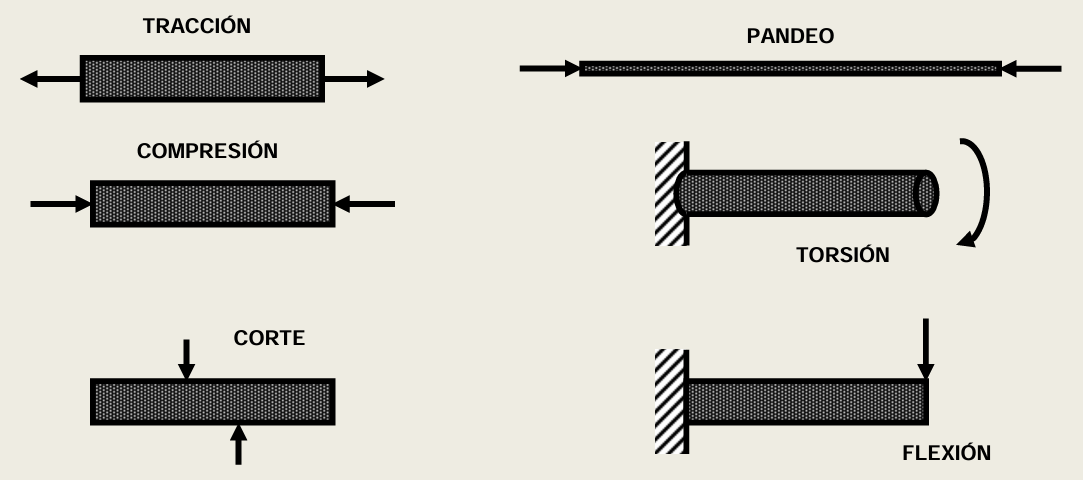
\includegraphics[width=0.7\textwidth]{Tipos_carga.png}
              \caption{Fuente: Transparencias Asignatura}
              \label{fig:tipos_carga}
          \end{figure}

    \item \textbf{Superficie y distribución de aplicación:} Carga concentrada (puntual), uniformemente distribuida o uniformemente variada.
          \begin{figure}[H]
              \centering
              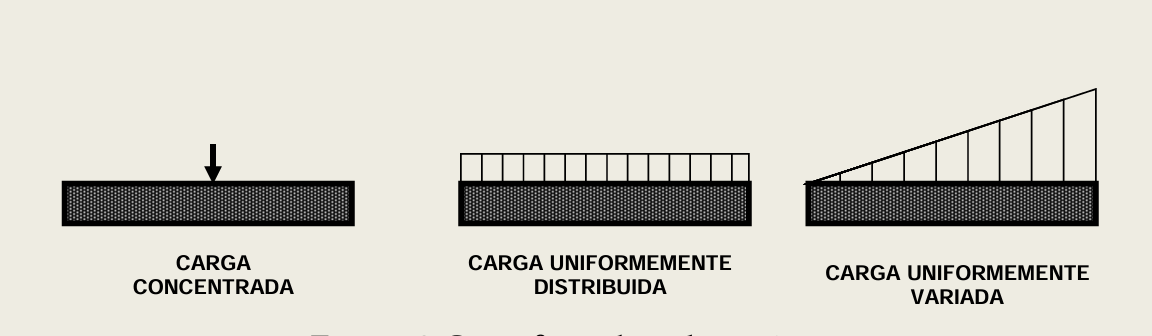
\includegraphics[width=0.7\textwidth]{superficie_aplicacion.png}
              \caption{Fuente: Transparencias Asignatura}
              \label{fig:superficie_aplicacion}
          \end{figure}
    \item \textbf{Tiempo y régimen de duración:}
          \begin{itemize}
              \item \textit{Carga constante o estática:} Aplicada de forma suave y mantenida en el tiempo.
              \item \textit{Carga progresiva:} Crecimiento lento y continuo de la solicitación.
              \item \textit{Carga repetitiva o cíclica:} Cargas variables en el tiempo que oscilan o fluctúan (origen de la fatiga).
              \item \textit{Carga alternativa:} Fluctuación completa del sentido de la carga (de $+P$ a $-P$).
              \item \textit{Carga de choque o impacto:} Aplicación brusca en fracciones de segundo con elevada transferencia de energía cinética.
          \end{itemize}
    \item \textbf{Condiciones del medio:} Temperatura de servicio (criogénica o elevada), exposición a atmósferas húmedas, salinas o fluidos corrosivos bajo tensión.
\end{enumerate}
\subsection{propiedades mecánicas}
El comportamiento mecánico de un material refleja la relación entre la fuerza aplicada y la respuesta del material a su deformación (resistencia que ofrece a la aplicación de la carga).
Las propiedades mecánicas de los materiales se determinan realizando ensayos normalizados que permiten comparar entre si el comportamiento de distintos materiales.
\begin{itemize}
    \item \textbf{Propiedades mecánicas de resistencia:} Comportamiento frente a esfuerzos axiales, cortantes o flectores (tracción, compresión, fatiga, termofluencia).
    \item \textbf{Propiedades mecánicas superficiales:} Resistencia a la deformación plástica localizada, penetración y rayado (dureza y resistencia al desgaste abrasivo).
    \item \textbf{Propiedades tecnológicas:} Capacidad del material para someterse a procesos de conformado y transformación (soldabilidad, flexión, embutición, abocardado).
\end{itemize}
Algunas normativas que lo regulan son ASME, ASTM y ISO.
\subsection{Conceptos Básicos de Elasticidad y Deformación}

\subsubsection{Tensión o Esfuerzo ($\sigma$)}
\dfn{Tensión o esfuerzo nominal}{Es la resistencia interna que ofrece una sección del material perpendicular a la carga aplicada. La tensión o esfuerzo que sufre un elemento ($\sigma$) es igual al cociente entre la fuerza uniaxial media y la sección transversal original de la barra.}

Considerando una barra o probeta prismática/cilíndrica de longitud inicial $l_0$ y sección transversal inicial $A_0$ sometida a una fuerza uniaxial normal $P$, la tensión $\sigma$ viene dada por:
\begin{equation}
    \sigma = \frac{P}{A_0}
    \label{eq:tension_nominal}
\end{equation}
\nt{La tensión ingenieriel siempre esta referida a la sección inicial}
\textbf{Unidades de tensión y esfuerzo habituales en ingeniería:}
\begin{itemize}
    \item \textbf{Sistema Internacional (SI):} Pascal ($\text{Pa} = \text{N}/\text{m}^2$). En ingeniería mecánica se emplean los múltiplos:
          \begin{equation*}
              1\text{ MPa} = 10^6\text{ Pa} = 1\text{ N}/\text{mm}^2, \qquad 1\text{ GPa} = 10^9\text{ Pa} = 10^3\text{ N}/\text{mm}^2
          \end{equation*}
    \item \textbf{Sistema Técnico:} Kilogramo-fuerza por centímetro cuadrado ($\text{kgf}/\text{cm}^2$) o por milímetro cuadrado ($\text{kgf}/\text{mm}^2$), donde $1\text{ kgf} \approx 9.80665\text{ N}$.
    \item \textbf{Sistema Anglosajón (U.S. Customary Units):} Libra-fuerza por pulgada cuadrada ($\text{psi} = \text{lbf}/\text{in}^2$) o miles de psi ($\text{ksi} = 10^3\text{ psi}$):
          \begin{equation*}
              1\text{ psi} \approx 6.89476 \times 10^3\text{ Pa}, \qquad 1\text{ ksi} \approx 6.89476\text{ MPa}
          \end{equation*}
\end{itemize}

\subsubsection{Deformación y Deformación Unitaria ($\varepsilon$)}
\dfn{Deformación}{Al aplicar una carga uniaxial $P$, el elemento experimenta una variación dimensional en la dirección longitudinal de la fuerza denominada alargamiento o deformación total $\delta = l - l_0$. Es decir es el incremento de la longitud de la barra o probeta inicial. }

\dfn{Deformación Unitaria}{En ingeniería se define la \textbf{deformación unitaria nominal} ($\varepsilon$) como el cociente entre el incremento de longitud y la longitud inicial de referencia:}
\begin{equation}
    \varepsilon = \frac{\delta}{l_0} = \frac{l - l_0}{l_0} \quad [\text{adimensional, habitualmente expresada en } \% \text{ o en } \text{mm}/\text{mm}]
    \label{eq:deformacion_unitaria}
\end{equation}

\subsubsection{Coeficiente de Poisson ($\nu$ o $\eta$)}
Una deformación longitudinal uniaxial viene invariablemente acompañada por una deformación transversal de sentido opuesto (contracción lateral en tracción, dilatación lateral en compresión). En materiales elásticos homogéneos e isótropos, las deformaciones unitarias transversales en los ejes perpendiculares son iguales ($\varepsilon_x = \varepsilon_y$).

El \textbf{coeficiente de Poisson} se define como el valor negativo del cociente entre la deformación unitaria lateral y la deformación unitaria longitudinal axial ($\varepsilon_z$):
\begin{equation}
    \nu = -\frac{\varepsilon_x}{\varepsilon_z} = -\frac{\varepsilon_y}{\varepsilon_z}
    \label{eq:poisson_ratio}
\end{equation}

Para un material idealmente incompresible bajo deformación elástica (sin variación de volumen), $\nu = 0.50$. En los materiales estructurales y metales de interés en ingeniería mecánica, $\nu$ oscila habitualmente entre $0.25$ y $0.40$ (Tabla~\ref{tab:poisson_valores}).

\begin{table}[H]
    \centering
    \begin{tabular}{lc lc}
        \toprule
        \textbf{Metal / Aleación} & \textbf{Coeficiente $\nu$} & \textbf{Metal / Aleación}     & \textbf{Coeficiente $\nu$} \\
        \midrule
        Aluminio                  & 0.33                       & Latón                         & 0.35                       \\
        Cobre                     & 0.35                       & Magnesio                      & 0.29                       \\
        Níquel                    & 0.31                       & Acero ordinario / estructural & 0.27 -- 0.30               \\
        Titanio                   & 0.36                       & Tungsteno (Wolframio)         & 0.28                       \\
        \bottomrule
    \end{tabular}
    \caption{Coeficientes de Poisson característicos para metales y aleaciones habituales.}
    \label{tab:poisson_valores}
\end{table}

\subsubsection{Deformación Elástica frente a Deformación Plástica}
Al someter a una fuerza de tensión uniaxial $\sigma$, el material sufre deformación, dependiendo de como quede el material despues de retirarla podemos hablar de:

\begin{itemize}
    \item \textbf{Deformación elástica:} Si al retirar la carga el material recupera instantáneamente sus dimensiones iniciales $l_0$.
    \item \textbf{Deformación plástica:} Si al retirar la carga el material experimenta una deformación permanente y residual. Durante esta deformación se ha producido una reorganización estructural del material y los atomos se han desplazado de sus posiciones de equilibrio.
\end{itemize}
\newpage
\section{Ensayo de Tracción}

El ensayo de tracción uniaxial es el procedimiento estándar más importante para determinar cuantitativamente las propiedades mecánicas de resistencia y deformabilidad de los materiales.

Se someten a un lento estiramiento mediante una equipo de ensayo \ref{fig:ensayo_traccion_esquema}, observándose la carga resultante y la deformación unitaria obtenida hasta el momento de la rotura final de la pieza. Debido a que las tensiones son monoaxiales y no poliaxiales tal y como se dan en la realidad
este ensayo \textbf{No proporciona conclusiones definitivas, Pero es clave para comparar diferentes materiales entre si, ademas las condiciones a las que se realiza el ensayo deben estar normalizadas} es decir se usan probetas de dimensiones establecidas, ademas de a una velocidad y temperatura prefijadas.

\begin{figure}[H]
    \centering
    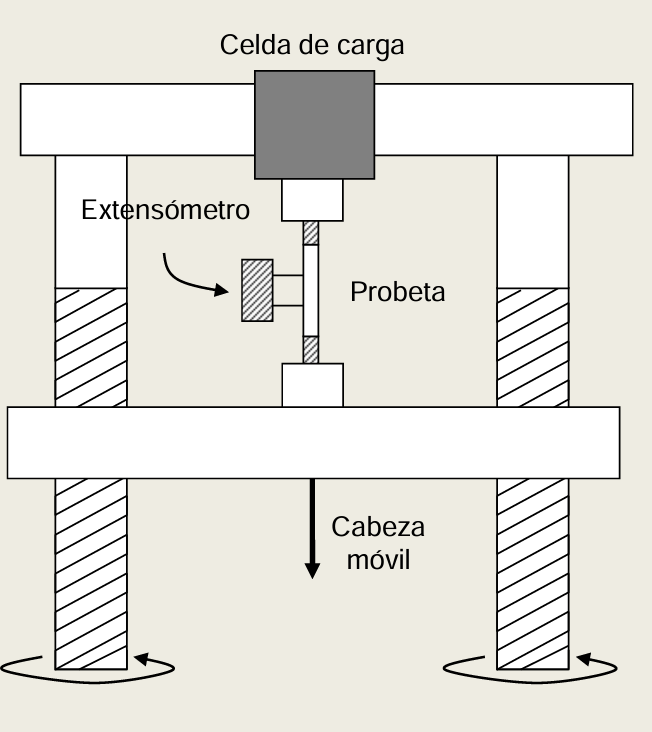
\includegraphics[width=0.7\textwidth]{ensayo_traccion.png}
    \caption{Esquema del ensayo de tracción.\\ Fuente: Transparencias Asignatura}
    \label{fig:ensayo_traccion_esquema}
\end{figure}

\subsection{Probetas Normalizadas (Norma ASTM)}
Para garantizar la reproducibilidad y comparación interlaboratorio, el ensayo se realiza bajo condiciones normalizadas (velocidad de deformación controlada y temperatura ambiente controlada). La Sociedad Americana de Ensayos de Materiales (\textbf{ASTM}) especifica geometrías estandarizadas:
\begin{itemize}
    \item \textbf{Probetas de sección circular:} Utilizadas comúnmente en piezas forjadas, barras y fundiciones. Presentan una longitud calibrada central reducida de diámetro $d_0 = 0.500'' \pm 0.010''$ ($12.7\text{ mm}$) y una longitud de calibración $L_0 = 2.000'' \pm 0.005''$ ($50.8\text{ mm}$). \textcolor{red}{En general, se exige la condición geométrica:} \nt{En caso de que la relación sea mayor}
          \begin{equation}
              \frac{L_0}{d_0} \leqslant 4
          \end{equation}
    \item \textbf{Probetas de sección rectangular:} Utilizadas para ensayos de chapas, perfiles y láminas laminadas, adaptando el espesor al del producto comercial y con transiciones curvas amplias hacia los cabezales de amarre.
\end{itemize}
Los extremos ensanchados de la probeta se sujetan mediante mordazas de cuña, asegurando que la rotura ocurra siempre en la zona central calibrada y no en las proximidades de las mordazas donde se generan concentraciones locales de tensiones.

\subsection{Curva Tensión-Deformación y Puntos Característicos}

Si se coloca la probeta en la máquina de ensayo de tracción y compresión y se aplica gradualmente \textbf{fuerzas de tracción} en los extremos, se puede medir \textbf{el alargamiento total en la longitud patrón para cualquier incremento predeterminado de la carga axial.} Las máquinas llevan generalmente un dispositivo que representa en un diagrama \textbf{la relación entre la carga (P) y el alargamiento ($\delta$).} Normalmente en los diagramas tensióndeformación se representa el \textbf{esfuerzo desarrollado en la probeta ($\sigma$) frente a la deformación unitaria ($\epsilon$)}

\begin{figure}[H]
    \centering
    \includegraphics[width=0.7\textwidth]{diagrama_tension_deformacion.png}
    \caption{Diagrama tensión-deformación para distintos materiales. Fuente: Transparencias Asignatura}
    \label{fig:diagrama_tension_deformacion}
\end{figure}
\begin{itemize}
    \item \textbf{Materiales dúctiles (a)} (ej. aceros de bajo carbono, cobre, aluminio recocido): Presentan un alargamiento elástico inicial lineal, una clara zona de deformación plástica uniforme generalizada, estricción localizada y un elevado alargamiento total antes de la fractura (Punto de rotura).
    \item \textbf{Materiales frágiles (b)} (ej. fundiciones grises, cerámicos, aceros de altísima dureza): Prácticamente no exhiben deformación plástica; la rotura se produce de manera repentina poco después de superado el régimen elástico lineal, con deformación a rotura insignificante.
    \item \textbf{Materiales elastoméricos / polímeros termoplásticos (c):} Muestran curvas no lineales con grandes deformaciones como se aprecia en la gráfica.
\end{itemize}
\nt{En el eje y siempre debe ir la tensión ingenieril es decir respecto a la sección inicial}
Del diagrama se pueden obtener una serie de puntos claves que caracterizan a los materiales como son:
\begin{multicols}{2}
    \begin{itemize}
        \item Límite de proporcionalidad elástico
        \item Límite elástico
        \item Puntos de fluencia
        \item Resistencia máxima a la tracción
        \item Punto de rotura
        \item Ductilidad
        \item Resiliencia
        \item Tenacidad
    \end{itemize}
\end{multicols}
\begin{figure}
    \centering
    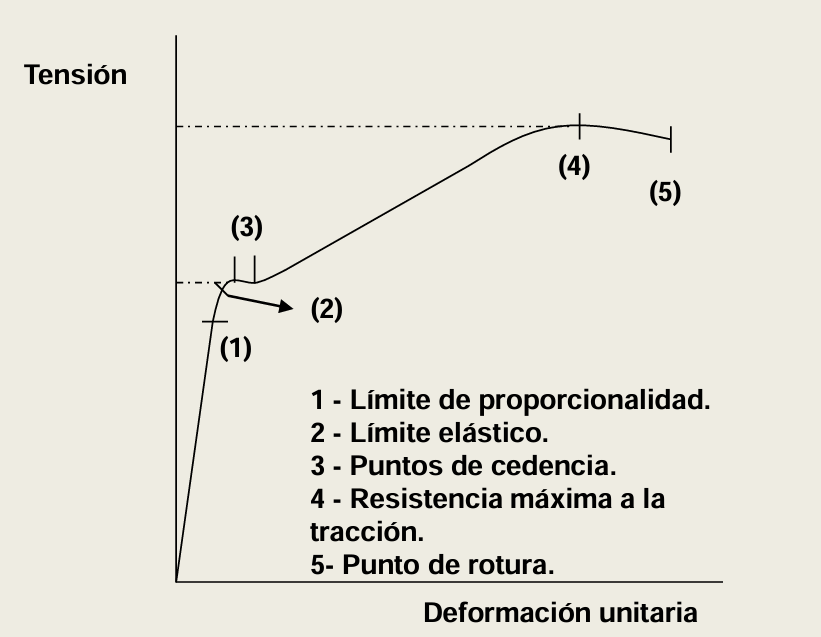
\includegraphics[width=0.7\textwidth]{puntos_diagrama_tension_deformacion.png}
    \caption{Puntos característicos de la curva tensión-deformación del acero.\\ Fuente: Transparencias Asignatura}
    \label{fig:puntos_diagrama_tension_deformacion}
\end{figure}
Estos puntos son importantes, ya que nos permiten determinar la tensión maxima para el diseño del equipo, aunque dependiendo del caso se optará por unos puntos u otros.
\subsubsection{Módulo de Young ($E$) y Límite de Proporcionalidad ($\sigma_{LP}$)}
Es la relacion entre la tensión $\sigma$ y la deformación $\varepsilon$, se calcula en el tramo inicial de la curva donde la relación es estrictamente proporcional cumpliéndose la \textbf{Ley de Hooke}:
\begin{equation}
    \sigma = E \, \varepsilon \quad \Longleftrightarrow \quad \frac{P}{A_0} = E \, \frac{\delta}{L_0}
    \label{eq:hooke_law}
\end{equation}
La constante de proporcionalidad $E$ se denomina \textbf{Módulo de Elasticidad o Módulo de Young}. Representa la rigidez del material frente a la deformación elástica:
\begin{itemize}
    \item Un valor elevado de $E$ indica un material rígido (requiere elevados esfuerzos para sufrir deformación elástica).
    \item Un valor bajo de $E$ describe un material flexible o elástico.
\end{itemize}

\begin{table}[H]
    \centering
    \begin{tabular}{lccc}
        \toprule
        \textbf{Material}                  & \textbf{$E$ ($\text{psi}$)} & \textbf{$E$ ($\text{GPa}$)} & \textbf{$E$ ($\text{Pa}$)} \\
        \midrule
        Cobre recocido                     & $16 \times 10^6$            & $110$                       & $1.1 \times 10^{11}$       \\
        Acero ordinario y de baja aleación & $29 \times 10^6$            & $200$                       & $2.0 \times 10^{11}$       \\
        Aleaciones de aluminio estructural & $10 \times 10^6$            & $70$                        & $0.7 \times 10^{11}$       \\
        Titanio comercial puro             & $15 \times 10^6$            & $105$                       & $1.05 \times 10^{11}$      \\
        \bottomrule
    \end{tabular}
    \caption{Módulos de Young característicos para distintos metales de uso en ingeniería.}
    \label{tab:modulos_young}
\end{table}

\dfn{Límite de proporcionalidad ($\sigma_{LP}$)}{El \textbf{límite de proporcionalidad} ($\sigma_{LP}$) representa el nivel máximo de tensión a partir del cual la relación lineal deja de cumplirse:}
\begin{equation}
    \sigma_{LP} = \frac{P_{LP}}{A_0}
\end{equation}
\imp{La tensión en el límite de proporcionalidad ($\sigma_{LP}$) es la correspondiente al punto donde deja de existir una relación lineal entre el esfuerzo aplicado y la deformación unitaria. $P_{LP}$ es la carga aplicada en el límite de proporcionalidad.}
\textbf{Método de Johnson para determinar $\sigma_{LP}$:} Dado que la desviación de la linealidad puede ser gradual y difícil de discernir visualmente, se emplea el método gráfico de Johnson: se traza una recta $OE$ tangente a la curva en el origen con pendiente $E$, y se define otra recta $OD$ con una pendiente un $50\%$ inferior respecto al eje de esfuerzos (es decir, en una paralela horizontal a distancia $FD = 1.5 \, FE$). Trazando una paralela a $OD$ que sea tangente a la curva de tracción, el punto de tangencia define con rigor el límite de proporcionalidad.
\begin{figure}[H]
    \centering
    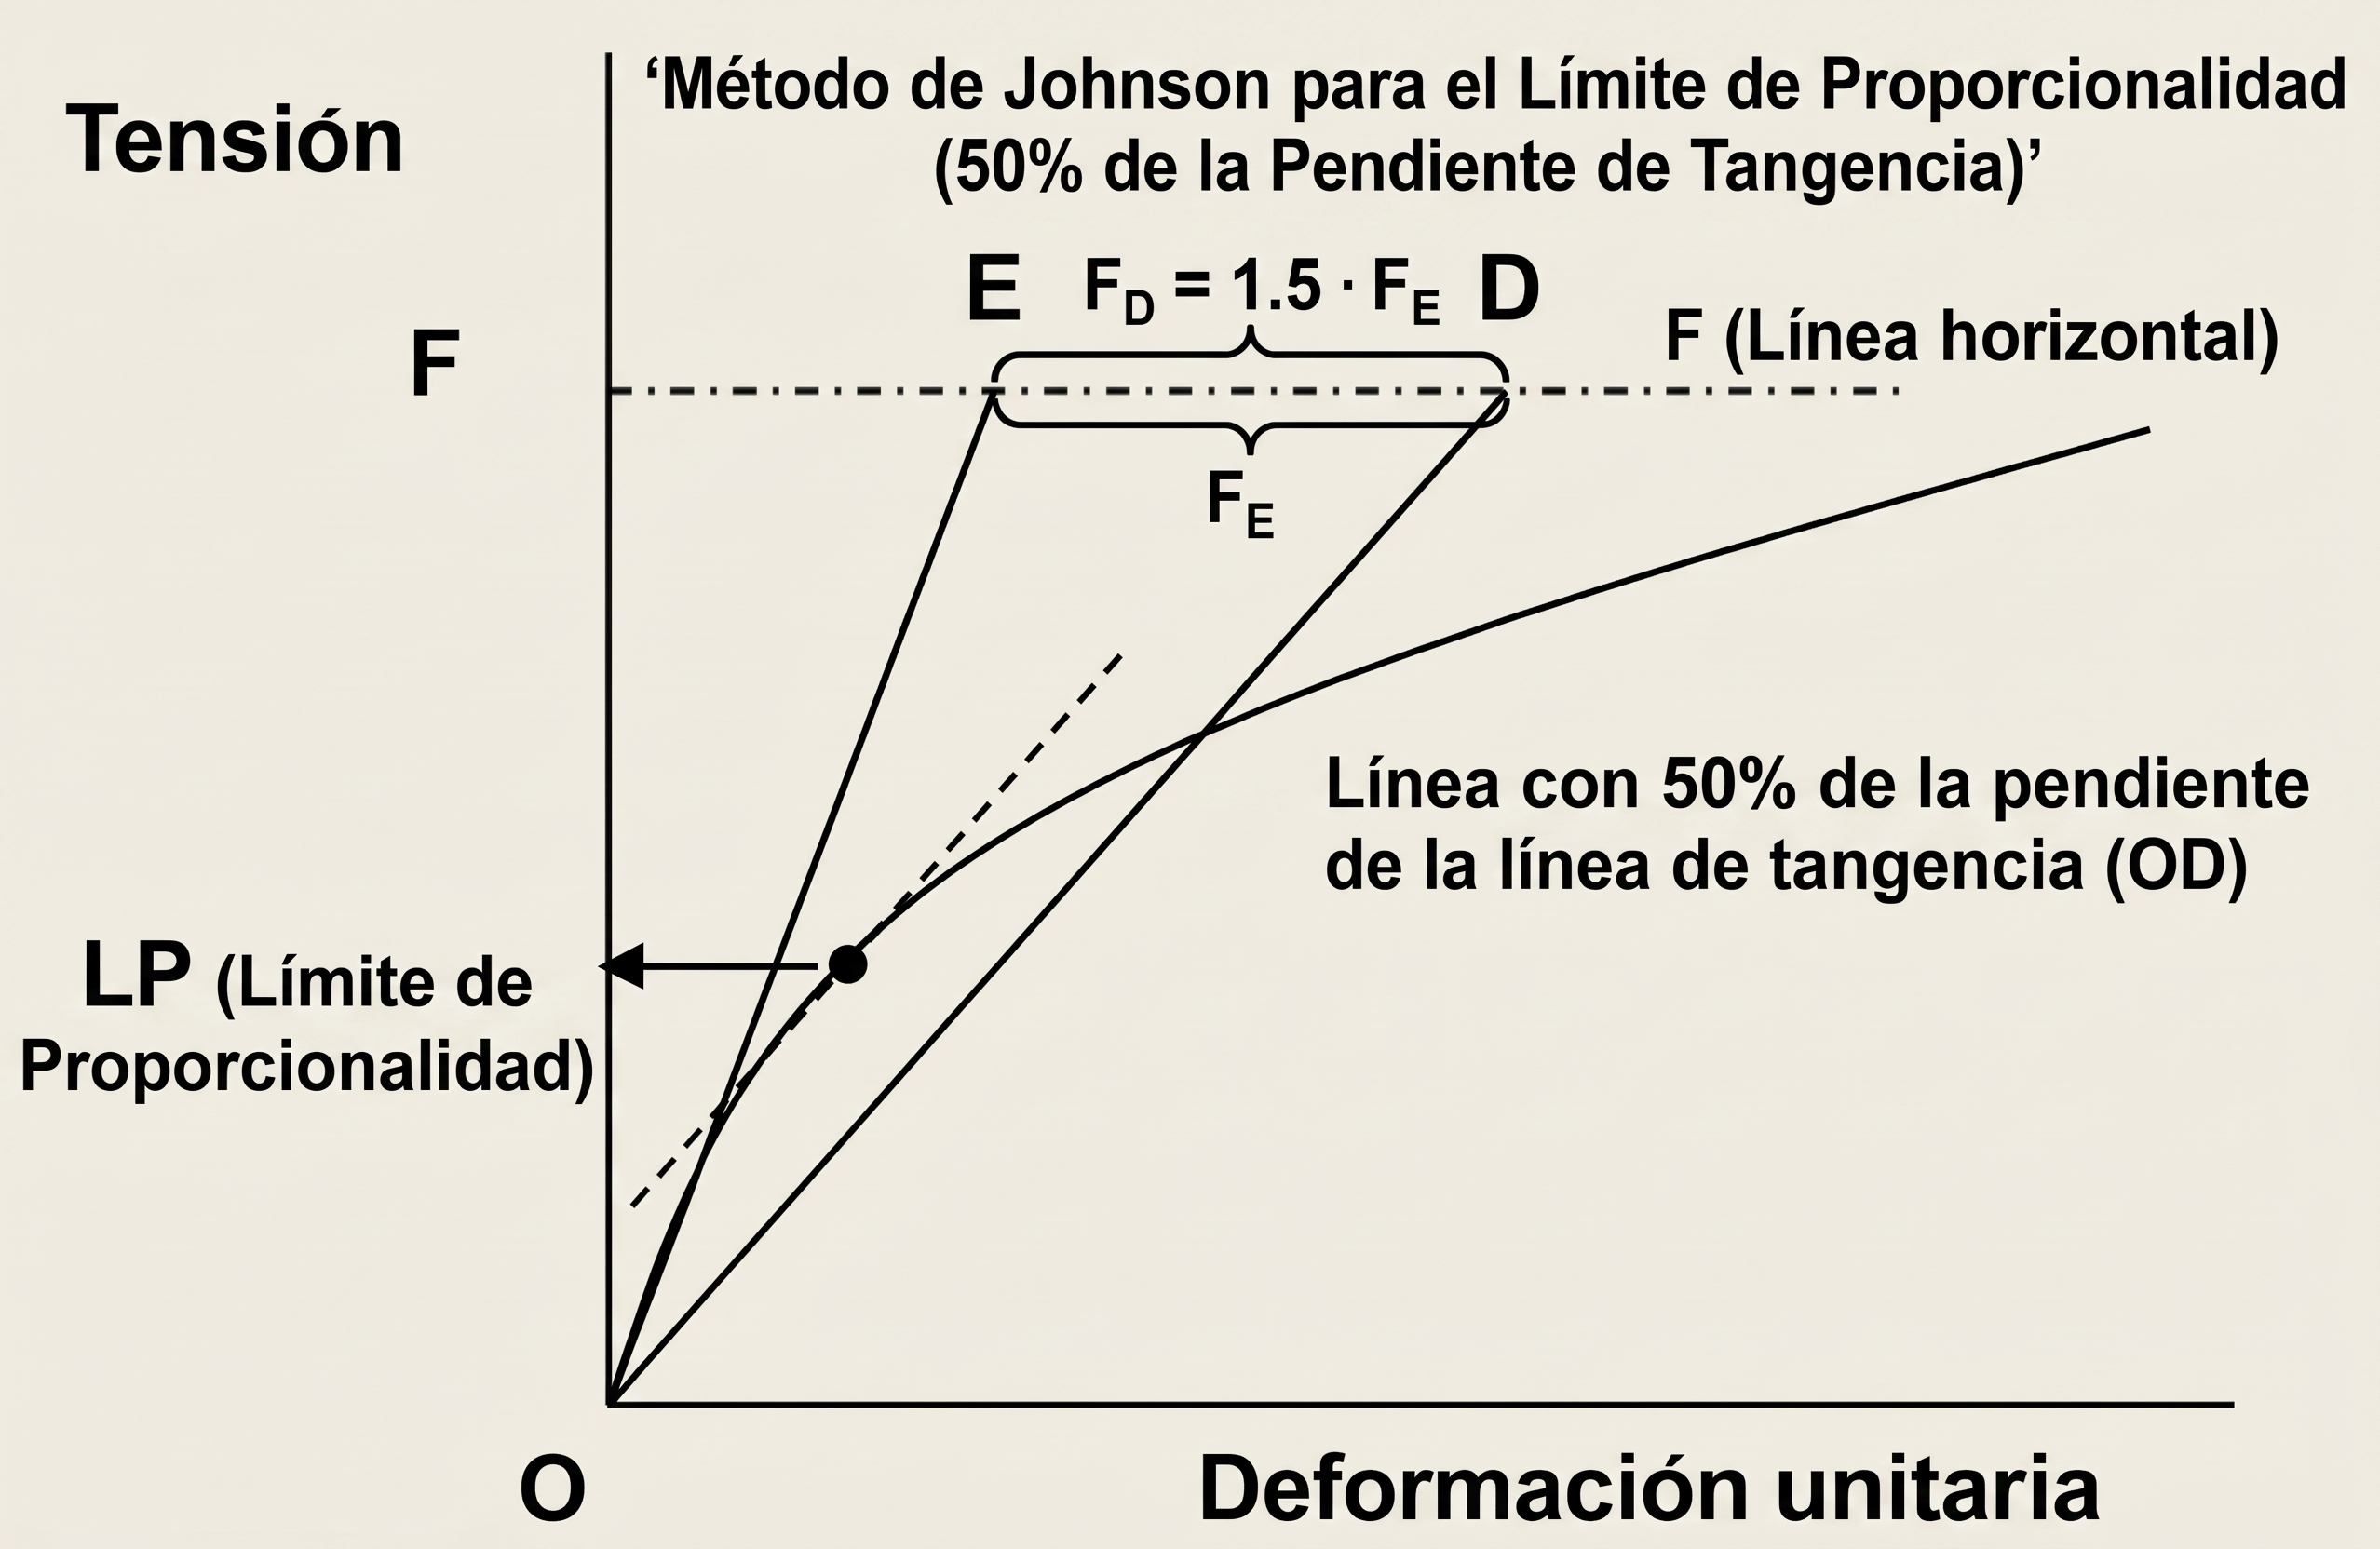
\includegraphics[width=0.7\textwidth]{Gemini_Generated_Image_a8mnpsa8mnpsa8mn.jpg}
    \caption{Método de Johnson para determinar $\sigma_{LP}$. Fuente: Transparencias Asignatura}
    \label{fig:metodo_johnson}
\end{figure}
\subsubsection{Límite de Elasticidad ($\sigma_{LE}$)}
Es la tensión máxima admisible sin que se produzcan deformaciones permanentes al cesar la carga. Generalmente coincide con el límite de proporcionalidad y se evalúa a partir de la siguiente expresión:
\begin{equation}
    \sigma_{LE} = \frac{P_{LE}}{A_0}
\end{equation}
donde \textbf{$P_{LE}$ es la carga aplicada en el límite de elasticidad.} Si al material ensayado se le aplica una carga superior sufrira una deformación plástica, por lo general se suele trabajar por debajo del limite de elasticidad (teniendo tambien en cuenta un coeficiente de seguridad).

\subsubsection{Límite o Punto de Fluencia / Cedencia ($\sigma_{LF}$ o $\sigma_A$)}
Es el valor de tensión a partir del cual el material experimenta un alargamiento considerable sin necesidad de aumentar la carga exterior.

Algunas veces la fluencia viene acompañada de un descenso en la tensión y en ese caso se aprecian dos puntos de fluencia:
\begin{itemize}
    \item \textbf{Punto de fluencia superior ($\sigma_{LFs} = P_A/A_0$):} \textbf{Depende de la forma con la que se realiza el ensayo}, es decir de la geometría de la probeta y de la velocidad de aplicación del ensayo.
    \item \textbf{Punto de fluencia inferior ($\sigma_{LFi} = P_B/A_0$):} \textbf{Es una propiedad intrínseca del material}, es decir es un punto característico del material.
\end{itemize}

\textbf{Convención de fluencia al 0.2\% ($\sigma_{0.2}$):} En aquellos materiales que no presentan un escalón de fluencia pronunciado (como los aceros de alta aleación, cobres, latones o aleaciones de aluminio), se define el límite elástico convencional como la tensión que genera una deformación plástica permanente remanente del $0.2\%$ ($\varepsilon = 0.002\text{ mm}/\text{mm}$). Se calcula trazando una recta paralela al tramo lineal elástico que parte desde la abscisa $\varepsilon = 0.002$; la intersección con la curva define el punto de fluencia de diseño.
\dfn{Tensión de fluencia sin límite definido obvio:}{Esfuerzo desarrollado en la probeta que provoca sobre el material una deformacion permanente del 0.2\%}
\subsubsection{Resistencia Máxima a la Tracción ($\sigma_M$ o $S_u$)}
Si se aumenta la carga aplicada sobre la probeta mas allá del punto de fluencia,es decir a medida que la probeta sigue deformándose plásticamente, experimenta endurecimiento por deformación hasta alcanzar la carga máxima admisible $P_M$. La resistencia última a la tracción referida a la sección inicial es:
\begin{equation}
    \sigma_M = \frac{P_M}{A_0}
\end{equation}
Una vez superado el punto de resistencia máxima, la deformación plástica deja de ser homogénea a lo largo de toda la longitud calibrada y se concentra en una zona restringida, originándose el fenómeno de \textbf{estricción} (formación de un cuello o garganta donde el área transversal real disminuye drásticamente). Debido a esta rápida reducción de área transversal, la carga global $P$ requerida para continuar el estiramiento decrece de forma aparente.
\nt{Correspone al punto M, que representa la resistencia máxima a tracción del material referida a la sección inicial de la probeta}
\newpage
\subsubsection{Punto y Tensión de Rotura ($\sigma_D$)}
Corresponde al punto final donde la probeta fractura definitivamente bajo una carga D.
\begin{figure}[H]
    \centering
    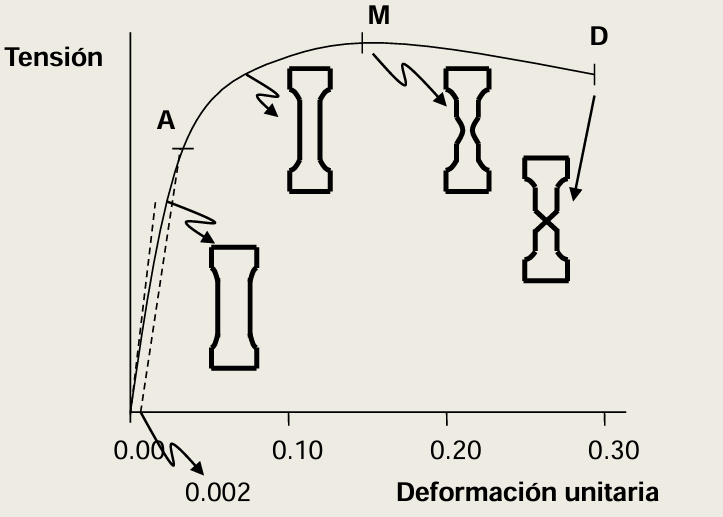
\includegraphics[width=0.7\textwidth]{punto_rotura.png}
    \caption{Resistencia máxima y punto de rotura \\ Fuente: Transparencias Asignatura}
    \label{fig:punto_rotura}
\end{figure}
\subsubsection{Ductilidad: Alargamiento y Estricción a la Rotura}
\dfn{Ductilidad:}{Grado de deformación plástica que puede soportar un material antes de su fractura.}
La ductilidad se determina cuantitativamente mediante el Alargamiento a la rotura (AR) y la Estricción a la rotura (ER) a partir de los datos obtenidos tras un ensayo de tracción con las siguientes expresiones:
\begin{enumerate}
    \item \textbf{Porcentaje de alargamiento a la rotura (\%AR):}
          \begin{equation}
              \%AR = \frac{l_f - l_0}{l_0} \times 100
              \label{eq:porcentaje_ar}
          \end{equation}
    \item \textbf{Porcentaje de estricción (\%ES):}
          \begin{equation}
              \%ES = \frac{A_0 - A_f}{A_0} \times 100
              \label{eq:porcentaje_es}
          \end{equation}
\end{enumerate}
donde $l_0$ y $A_0$ son la longitud calibrada y la sección inicial, y $l_f$ y $A_f$ son la longitud final entre puntos calibrados y la sección transversal mínima en el cuello de rotura.
\nt{A mayores valores de \%AR y \%ES, mayor es la ductilidad del material y su seguridad frente a roturas catastróficas.}
\begin{itemize}
    \item \textbf{Material frágil:} aquel que no puede tener apenas deformación plástica antes de romperse, se rompen de golpe, sin avisar. Por ejemplo el vidrio. Los materiales frágiles son aquellos que no han sufrido deformación plástica antes de romperse (se rompen justo en el límite elástico).
    \item \textbf{Material dúctil:} aquel que puede tener grandes deformaciones plásticas antes de romperse
\end{itemize}
\subsubsection{Resiliencia y Módulo de Resiliencia}
\dfn{Resiliencia:}{Es la capacidad de un material de absorber energía elástica cuando es deformado y devolverla íntegramente al retirar la carga exterior.}
\nt{Representa el área bajo el tramo elástico de la curva tensión-deformación hasta el límite de proporcionalidad.}

La energía de deformación elástica acumulada en el volumen de la probeta es el trabajo desarrollado por la fuerza:
\begin{equation}
    U = \frac{1}{2} P_{LP} \, \delta_{LP} \quad \xRightarrow{\text{Con la def. de }\sigma_{LP} \text{ y la ley de Hooke}} \frac{1}{2} \left(\frac{\sigma_{LP}^2}{E}\right) A_0 \, L_0
\end{equation}
El \textbf{Módulo de Resiliencia} ($U_r$) se define como la energía elástica absorbida por unidad de volumen de material:
\begin{equation}
    U_r = \frac{U}{A_0 \, L_0} = \frac{1}{2} \, \frac{\sigma_{LP}^2}{E}
    \label{eq:modulo_resiliencia}
\end{equation}
\textbf{Esta propiedad cuantifica la resistencia frente a choques a baja velocidad} y para maximizarla se requieren materiales con elevado límite elástico $\sigma_{LP}$ y bajo módulo elástico $E$.

\subsubsection{Tenacidad y Ensayos de Impacto (Charpy e Izod)}
\dfn{Tenacidad:}{Es la capacidad de un material de absorber energía mecánica elástica y plástica antes de que se produzca la fractura.}
Representa la energía máxima absorbida por unidad de volumen antes de originarse la ruptura total del material, se puede obtener de las siguientes formas:
\begin{itemize}
    \item Corresponde al área total bajo la curva completa tensión-deformación hasta el punto de rotura. Puede estimarse analíticamente de forma aproximada mediante la regla del trapecio:
          \begin{equation}
              \text{Tenacidad} \approx \frac{\sigma_A + \sigma_M}{2} \cdot \delta_D
              \label{eq:tenacidad_aprox}
          \end{equation}
          donde $\sigma_A$ es la tensión de fluencia, $\sigma_M$ la resistencia última y $\delta_D$ la deformación total a rotura.
    \item Evaluada mediante \textbf{ensayos normalizados de impacto en probetas entalladas (ensayos Charpy e Izod)}. Un martillo pendular de masa conocida se libera desde una altura inicial $h$, fractura la probeta entallada por flexión en un único golpe y asciende hasta una altura residual $h' < h$. La energía absorbida en el impacto es:
          \begin{equation}
              E_{\text{impacto}} = m g (h - h')
          \end{equation}
          \begin{itemize}
              \item \textit{Ensayo Charpy:} La probeta se apoya como viga simplemente apoyada en ambos extremos y el péndulo golpea en el centro por la cara opuesta a la entalla. Se utiliza típicamente en materiales dúctiles y aceros estructurales.
              \item \textit{Ensayo Izod:} La probeta se empotra verticalmente en voladizo y el péndulo golpea a una distancia fija en la cara donde se ubica la entalla. Muy empleado para plásticos y materiales más frágiles.
          \end{itemize}
\end{itemize}
\imp{La diferencia entre ambos ensayos es la forma de colocar la probeta. El ensayo de Izod se utiliza para determinar la tenacidad en materiales frágiles y el de Charpy para materiales dúctiles, ademas los resultados de los ensayos son cualitativos y se realizan con fines comparativos.}
\begin{figure}[H]
    \centering
    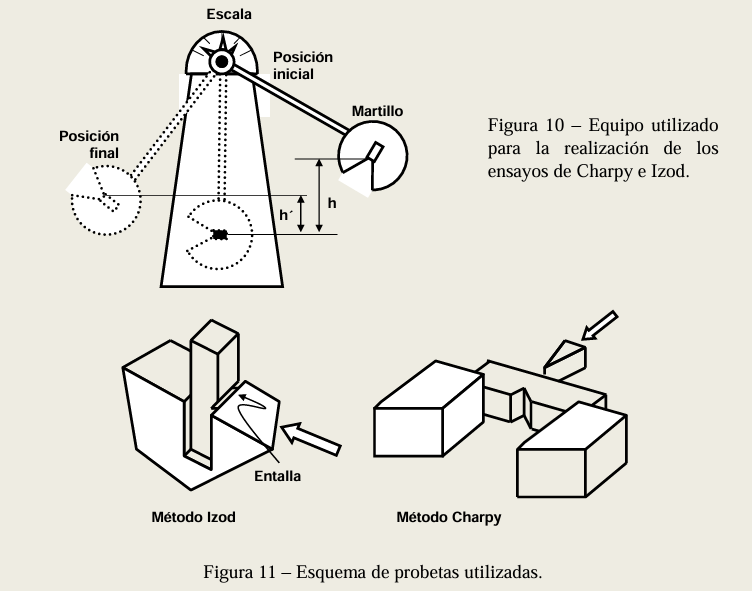
\includegraphics[width=0.6\textwidth]{ensayo_charpy_e_izod.png}
    \caption{Esquema del ensayo de \textbf{Charpy e Izod} \\ Fuente: Transparencias Asignatura}
    \label{fig:ensayo_charpy_e_izod}
\end{figure}
\paragraph{Transición Dúctil-Frágil y Efecto de la Temperatura:}
En metales con estructura cristalina cúbica centrada en el cuerpo (\textbf{BCC}, como los aceros al carbono ferríticos), la energía absorbida cae drásticamente al disminuir la temperatura, pasando de un comportamiento dúctil a alta absorción de energía a una rotura frágil y quebradiza por exfoliación a bajas temperaturas. Por el contrario, los metales con estructura cúbica centrada en las caras (\textbf{FCC}, como los aceros inoxidables austeníticos, aluminio, cobre y níquel) no presentan una transición brusca y retienen excelente tenacidad incluso a temperaturas criogénicas.

Asimismo, el contenido de carbono afecta de forma acusada: a medida que aumenta el porcentaje de carbono en los aceros recocidos, el material se vuelve más frágil, absorbe menos energía en el ensayo Charpy y el rango de transición hacia la fragilidad se desplaza a temperaturas más elevadas.
\imp{Es decir, en estos ensayos es importante la temperatura ya que puede haber una transición de ductil a fragil (cuando desciende la temperatura), ademas si cambiamos el contenido en carbono de los aceros recocidos se vuelven mas quebradizos y son capaces de absorber menos energía antes de su rotura.}
\begin{figure}[H]
    \centering
    \begin{subfigure}[c]{0.67\textwidth}
        \centering
        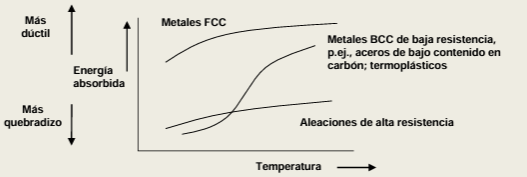
\includegraphics[height=4.2cm]{ductil_temperatura.png}
        \caption{Efecto de la temperatura en la tenacidad}
        \label{fig:ductil_temperatura}
    \end{subfigure}
    \hfill
    \begin{subfigure}[c]{0.3\textwidth}
        \centering
        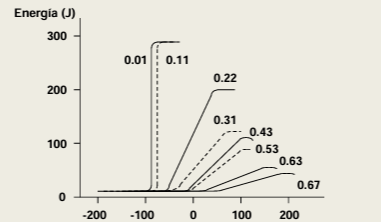
\includegraphics[height=4.2cm]{ductil_composicion.png}
        \caption{Efecto del porcentaje de carbono}
        \label{fig:ductil_composicion}
    \end{subfigure}
    \caption{Factores que influyen en la transición dúctil-frágil}
    \label{fig:ductil_transicion}
\end{figure}

\subsection{Tensiones y Deformaciones Reales}
En el cálculo convencional de ingeniería se utilizan el esfuerzo ingenieril $\sigma = P/A_0$ y la deformación ingenieril $\varepsilon = \delta/L_0$, es decir, se asume la sección inicial transversal a la aplicación de la carga para todos los calculos. Esto genera la falsa apariencia gráfica de que, superada la resistencia máxima, el material resiste menos esfuerzo. En la realidad física, el área transversal instantánea $A_i$ en la zona de estricción disminuye mucho más rápido que la carga aplicada, de modo que la tensión verdadera que soporta el material, \textbf{aumenta monótonamente hasta la rotura.}
\begin{figure}[H]
    \centering
    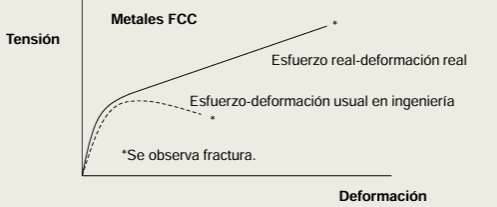
\includegraphics[width=0.7\textwidth]{deformacion_real.png}
    \caption{Tensión real vs Tensión ingenieril \\ Fuente: Transparencias Asignatura}
    \label{fig:deformacion_real}
\end{figure}
Se definen la \textbf{tensión real} ($\sigma_T$) y la \textbf{deformación real logarítmica} ($\varepsilon_T$) como:
\begin{equation}
    \sigma_T = \frac{P}{A_i}, \qquad \varepsilon_T = \int_{l_0}^{l_i} \frac{dl}{l} = \ln\left(\frac{l_i}{l_0}\right)
    \label{eq:tension_deformacion_reales}
\end{equation}
Asumiendo constancia de volumen durante la deformación plástica ($A_0 l_0 = A_i l_i$), se obtienen las relaciones de conversión válidas \textbf{hasta el comienzo de la estricción}:
\begin{equation}
    \sigma_T = \sigma \, (1 + \varepsilon), \qquad \varepsilon_T = \ln(1 + \varepsilon)
    \label{eq:conversion_real_nominal}
\end{equation}
\nt{Es decir que la tensión y deformación real estan relacionadas con las nominales(engenieriles) hasta que la probeta comienza a sufrir estricción.}
\paragraph{Ecuación constitutiva de Hollomon:}
En muchos metales y aleaciones, la región plástica comprendida entre el límite de fluencia y el comienzo de la estricción se ajusta fielmente a la ley potencial:
\begin{equation}
    \sigma_T = K \, \varepsilon_T^n
    \label{eq:hollomon}
\end{equation}
donde $K$ es el coeficiente de resistencia del material y $n$ es el \textbf{exponente de endurecimiento por deformación} ($n < 1$). A mayor valor de $n$, mayor es la capacidad del material para deformarse plásticamente de forma uniforme antes de que comience a localizarse la estricción (Tabla~\ref{tab:constantes_hollomon}).

\begin{table}[H]
    \centering
    \begin{tabular}{lcc}
        \toprule
        \textbf{Material}                     & \textbf{Exponente $n$} & \textbf{Constante $K$ ($\text{MPa}$)} \\
        \midrule
        Acero bajo en carbono (recocido)      & 0.26                   & 530                                   \\
        Acero aleado AISI 4340 (recocido)     & 0.15                   & 640                                   \\
        Acero inoxidable austenítico AISI 304 & 0.45                   & 1275                                  \\
        Aluminio recocido                     & 0.20                   & 180                                   \\
        Cobre recocido                        & 0.54                   & 315                                   \\
        Latón 70Cu-30Zn (recocido)            & 0.49                   & 895                                   \\
        Aleación de aluminio 2024-T4          & 0.16                   & 690                                   \\
        \bottomrule
    \end{tabular}
    \caption{Parámetros de endurecimiento por deformación ($n$ y $K$) para diversos materiales.}
    \label{tab:constantes_hollomon}
\end{table}

\subsection{Endurecimiento por Deformación Plástica (Acritud)}
Cuando un metal dúctil se somete a deformación plástica en frío (por encima de su límite elástico), la densidad de dislocaciones en su red cristalina se incrementa enormemente, multiplicándose y entorpeciendo su propio movimiento. \textbf{Es decir sufre una deformación plastica que produce un incremento de la resistencia elástica, tambien disminuye su ductilidad y aumenta su punto de fluencia.}

Si durante un ensayo de tracción se interrumpe la carga tras alcanzar una deformación plástica y se descarga el espécimen, el material desciende con una pendiente idéntica a la elástica ($E$). Al volver a aplicar carga, el material recorre el mismo camino elástico hasta alcanzar un \textbf{nuevo límite de fluencia significativamente más elevado} que el original.
\begin{figure}[H]
    \centering
    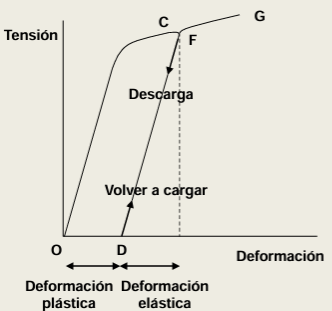
\includegraphics[width=0.5\textwidth]{endurecimiento_por_deformacion.png}
    \caption{Endurecimiento por deformación \\ Fuente: Transparencias Asignatura}
    \label{fig:endurecimiento_por_deformacion}
\end{figure}
\nt{En este grafico se observa como se le aplica una tensión inicial hasta recorriendo desde O hasta C, luego se descarga siguiendo la linea CD ya que al haber sufrido una deformación plastica no puede volver al estado original, siguiendo la trayectoria CD, al aplicar otra vez tensión seguira la trayectoria DF, siguiendo la ley de hooke hasta llegar a F y posteriormente si se sigue tensando habra un cambio brusco hasta G donde rompera.}
Este fenómeno confiere al material:
\begin{itemize}
    \item \textbf{Mayor rigidez y tensión elástica de servicio:} Se pueden aplicar cargas más altas sin que se genere nueva deformación plástica.
    \item \textbf{Aumento de la resistencia mecánica:} mejora unidireccional hacia donde se le aplico la carga, pero no mejora en el resto de las direcciónes del espacio.
    \item \textbf{Disminución de la ductilidad y de la tenacidad:} El material se torna más quebradizo.
    \item \textbf{Incremento del limite de proporcionalidad:} Aumenta la tensión necesaria para que el material comience a deformarse plásticamente.
    \item \textbf{Anisotropía:} El incremento de resistencia se produce preferentemente en la dirección en la que se aplicó la deformación uniaxial, pero no en las direcciones transversales.
    \item \textbf{Mayor susceptibilidad a la corrosión:} Las zonas con deformación plástica concentran tensiones residuales internas que aceleran la corrosión bajo tensión (aparece fluencia en las zonas no deformadas plásticamente).
\end{itemize}
El endurecimiento por deformación se puede revertir completamente restituyendo la ductilidad inicial mediante un \textbf{tratamiento térmico de recocido} a temperatura adecuada (tratamiento térmico suave a 100°C y posteriormente dejar enfriar lentamente).
\nt{Este tipo de tratamiento es común en procesos como el laminado de barras, estirado de tubos, ya que muchas veces se usa un material pretensado, es decir, se ha endurecido por acritud como se ha descrito previamente, un ejemplo sería en los pilares de hormigón pretensado, los cuáles son sometidos a esfuerzos de tracción para que se vuelvan más resistentes en dirección hacia donde sufrio la carga, aunque esto tiene un mayor coste economico.}
\section{Ensayo de Termofluencia (\textit{Creep})}

Muchos equipos de instalaciones químicas (\textbf{Reactores,turbinas}, calderas, intercambiadores de calor, columnas de destilación a presión y álabes de turbinas) operan simultáneamente bajo elevados esfuerzos mecánicos y altas temperaturas. A temperaturas elevadas las propiedades de los materiales experimentan cambios drásticos:
\begin{itemize}
    \item El módulo de elasticidad $E$ disminuye paulatinamente.
    \item El límite de proporcionalidad y la resistencia máxima a la tracción caen de forma notable a partir de cierta temperatura crítica.
    \item La ductilidad (\%AR y \%ES) se incrementa de forma acusada.
\end{itemize}

En estos equipos al sufrir una variación de temperatura importante, y tambien variación de presión (en especial en los reactores químicos de alta presión) las propiedades de los materiales pueden cambiar drásticamente, por lo que es importante conocer su comportamiento con este ensayo.

\subsection{Ensayo de tensión-deformación a distintas temperaturas}
\begin{figure}[H]
    \centering
    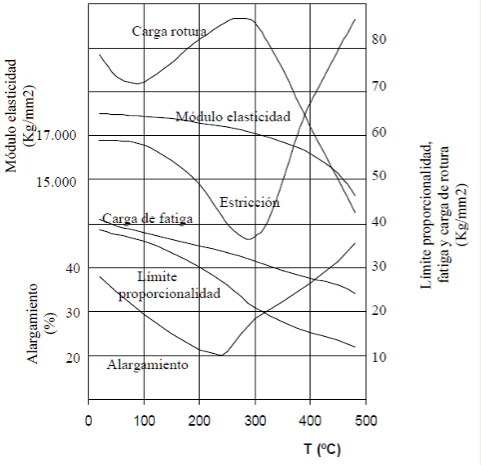
\includegraphics[width=0.5\textwidth]{termofluencia.png}
    \caption{Curva típica de termofluencia}
    \label{fig:termofluencia}
\end{figure}
En esta gráfica se puede observar la variación de las propiedades con la temperatura:
\begin{itemize}
    \item \textbf{Resistencia máxima a la tracción:} Crece hasta los 250\,°C.
    \item \textbf{Módulo de elasticidad:} Disminuye paulatinamente conforme aumenta la temperatura.
    \item \textbf{Contracción superficial (estricción):} Pasa por un mínimo a los 250\,°C y posteriormente crece de forma rápida.
    \item \textbf{Carga de fatiga:} Disminuye con la temperatura.
    \item \textbf{Límite de proporcionalidad:} Disminuye continuamente.
    \item \textbf{Alargamiento a la rotura:} Sigue un camino paralelo a la estricción ya que ambos definen la ductilidad (aumentan con la temperatura).
\end{itemize}

Los resultados de este ensayo arrojan la siguiente información:
\begin{itemize}
    \item Aquellas \textbf{propiedades que definen la ductilidad, como son la estricción y el alargamiento a la rotura, aumentan con la temperatura}
    \item las \textbf{propiedades relacionadas con la rigidez del material, como el límite de proporcionalidad y el módulo de elasticidad, disminuyen. La resistencia máxima a la tracción disminuye de forma apreciable tras una temperatura en específica}
\end{itemize}

\nt{En este gráfico se puede observar como la \textbf{resistencia a la tracción}} aumenta hasta los 250\,°C, mientras que el \textbf{módulo de elasticidad} disminuye de forma apreciable tras los 250\,°C, cabe mencionar que las \textbf{propiedades que definen la ductilidad, como son la estricción y el alargamiento a la rotura, aumentan con la temperatura}. Finalmente la \textbf{carga de fatiga} disminuye tras los 250\,°C.

Es importante considerar el tiempo como variable, ya que este ensayo es valido siempre y cuando  la carga actue durante un corto periódo de tiempo, si aumenta la duración (dias/semanas/meses) la carga necesaria para producir la rotura del material es cada vez mas pequeña.

\imp{para cargas que van a actuar durante largos períodos de tiempo y a temperaturas elevadas se necesitará una información más completa obtenida a partir de los ensayos termofluencia.}

\subsection{Ensayo de Termofluencia}
Bajo estas condiciones, la \textbf{variable tiempo} adquiere una importancia crítica. \textbf{Una pieza sometida a un esfuerzo constante inferior a su límite elástico puede sufrir una deformación plástica durante un cierto periodo de tiempo, esta deformación que depende del tiempo es conocida como termofluencia o fluencia lenta (\textit{creep})}.

\subsection{Curva Típica de Termofluencia y sus Etapas}
En un \textbf{ensayo} normalizado de \textbf{termofluencia}, una probeta se mantiene bajo \textbf{temperatura} rigurosamente controlada y \textbf{tensión} mecánica \textbf{constante}, registrando la \textbf{deformación en función del tiempo}. La curva característica presenta tres etapas bien diferenciadas:
\begin{enumerate}
    \item \textbf{Deformación elástica instantánea:} Es una deformación elástica instantánea que ocurre en el momento de aplicar la carga.
    \item \textbf{Etapa primaria o transitoria:} La probeta experimenta una deformación que aumenta progresivamente con el tiempo. el metal se endurece para soportar la carga aplicada por deformación, decreciendo la rapidez de la termofluencia con el tiempo a medida que el endurecimiento por deformación se hace más elevado.
    \item \textbf{Etapa secundaria o estacionaria:} La velocidad de deformación se mantiene prácticamente constante y mínima ($d\varepsilon/dt = \text{cte}$). En esta fase se establece un equilibrio dinámico entre el endurecimiento por deformación y los procesos térmicos de restauración y aniquilación de dislocaciones móviles promovidos por la difusión atómica. Tanto que el metal continúa alargandose a una velocidad constante, \textbf{La pendiente de esta región se denomina mínima rapidez de termofluencia}.
    \item \textbf{Etapa terciaria:} La velocidad de deformación se acelera de manera exponencial debido a la aparición de estricción macroscópica y la nucleación de microcavidades y grietas en los límites de grano, conduciendo rápidamente a la fractura del componente.
\end{enumerate}

la forma de la curva depende estrechamente de la carga y temperatura aplicada, Si existen esfuerzos y temperaturas elevadas, el tiempo necesario para la fractura del material disminuye de forma considerable.
\nt{Existen dos fenómenos importantes durante este proceso, un \textbf{endurecimiento del material provocado por la deformación plástica y un reblandecimiento causado al estar sometido a temperaturas elevadas.}}
\begin{figure}[H]
    \centering
    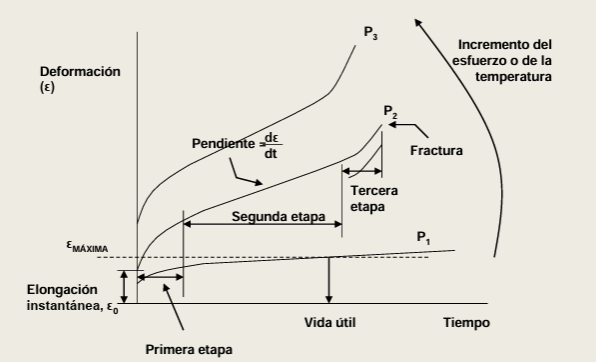
\includegraphics[width=0.7\textwidth]{ensayo_termofluencia.png}
    \caption{Curva típica de termofluencia}
    \label{fig:ensayo_termofluencia}
\end{figure}
Este ensayo se hace para materiales que soportaran altas temperaturas y cargas, como una turbina un reactor\dots
\imp{\textbf{La pendiente de la segunda etapa de la curva de termofluencia} es una medida que permite la comparación de diferentes materiales sometidos a las mismas condiciones del ensayo. El valor menor de la mínima rapidez de termofluencia una menor velocidad de deformación en esas condiciones.}
\nt{El esfuerzo que produce una \textbf{mínima rapidez de termofluencia de $10^{-5}\%/\text{h}$} también es otro parámetro que puede determinar la resistencia a la termofluencia e indicaría la evaluación de la carga máxima a aplicar al material a una determinada temperatura para que su velocidad de deformación fuese pequeña. \textbf{La elección de un material para trabajar a esfuerzo y temperaturas elevadas necesita de la realización de ensayos de termofluencia.} Este ensayo, junto con la \textbf{vida útil} del elemento, permite determinar fácilmente la \textbf{carga máxima} que puede ser aplicada sobre el material}
\section{Ensayo de Fatiga}

La \textbf{fatiga} es un mecanismo de degradación y \textbf{rotura} progresiva que se produce en piezas y componentes sometidos a tensiones dinámicas repetitivas, cíclicas o fluctuantes, por lo que el material falla con tensiones mucho mas pequeñas de las que podria soportar el material cuando se somete a cargas de tracción. \textbf{Es la primera causa de rotura de los materiales}

\textbf{Relevancia en ingeniería:} Representa la causa de más del $90\%$ de los fallos mecánicos en servicio en componentes metálicos. Lo más peligroso de la fatiga es que \textbf{la rotura sobreviene a tensiones notablemente inferiores a la resistencia estática de tracción e incluso por debajo del límite elástico, ocurriendo de forma súbita y sin deformación plástica previa apreciable}.

Las cargas aplicadas que producen fatiga pueden ser de distinta naturaleza: tracción, compresión, flexión o de naturaleza torsional. La resistencia que un material ofrece a la fatiga puede ser evaluada a partir de ensayos realizados en el laboratorio. Para ello la probeta se somete a esfuerzos alternativos de tracción y compresión de igual magnitud mediante el giro que provoca el equipo esquematizado, ademas las probetas son normalizadas. siguiendo el siguiente esquema
\nt{Suele ocurrir en equipos sometidos a presiones elevadas y tambien en ambientes corrosivos, otro ejemplo seria en un deposito donde se vacie y se llene continuamente.}
\subsection{Máquina de Ensayo y Curvas $S-N$ (Curvas de Wöhler)}
La resistencia a la fatiga se determina mediante ensayos dinámicos como el ensayo de flexión rotativa (máquina R.R.~Moore), en el que una probeta de sección calibrada gira a alta velocidad sometiéndose simultáneamente a tracción y compresión alternadas ($\sigma_{\text{med}} = 0$).

\begin{figure}
    \centering
    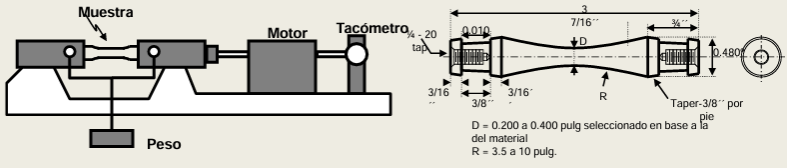
\includegraphics[width=0.7\textwidth]{ensayo_fatiga.png}
    \caption{Curva típica de fatiga}
    \label{fig:ensayo_fatiga}
\end{figure}

Los resultados se representan en un diagrama semilogarítmico de amplitud de tensión ($S$) frente al logaritmo del número de ciclos hasta la rotura ($N$):
\begin{itemize}
    \item \textbf{Materiales con límite de fatiga definido} (aceros al carbono y aleaciones de titanio): La curva $S-N$ se hace asintótica y totalmente horizontal a partir de un valor elevado de ciclos. Dicha asíntota define el \textbf{límite de fatiga} ($\sigma_e$ o $S_e$), que representa el nivel de tensión por debajo del cual el componente puede soportar un número infinito de ciclos sin romperse.
    \item \textbf{Materiales sin límite de fatiga definido} (aleaciones no férreas de aluminio, cobre, magnesio): La curva $S-N$ continúa descendiendo monótonamente. En este caso se define la \textbf{resistencia a la fatiga} para una vida prefijada de $N = 10^6$.
\end{itemize}

\begin{figure}
    \centering
    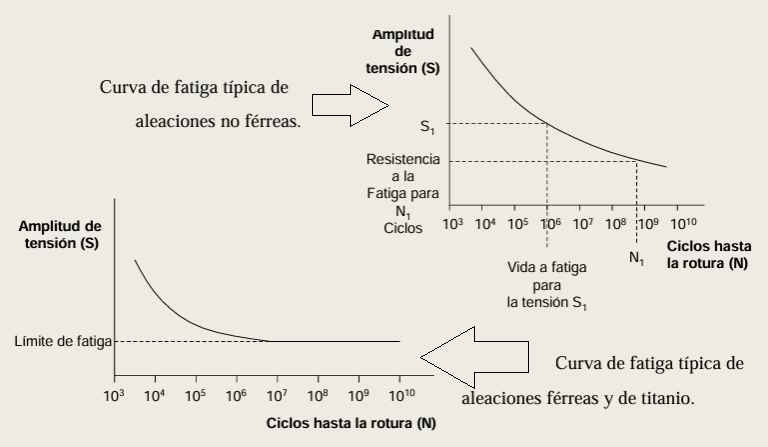
\includegraphics[width=0.7\textwidth]{curvas_fatiga.png}
    \caption{Curvas de fatiga para aleaciones ferricas y no ferricas. \\ Fuente: Callister, W. D. (2003). *Ciencia e Ingeniería de Materiales*. Grupo Editorial Iberoamericana.}
    \label{fig:curvas_fatiga}
\end{figure}
\imp{En resumen, los aceros al carbono y las aleaciones de titanio apresentam un límite de fatiga como la tensión para la cual el material puede someterse a infinitos ciclos. Otras aleaciones no férreas no presentan un límite de fatiga definido y para estos casos se define como la tensión de fatiga para la cual el material puede resistir hasta $10^6$ ciclos}
\subsection{Factores Críticos que Reducen la Vida a Fatiga}
La rotura por fatiga se inicia siempre en la superficie exterior y se propaga lentamente mediante microfisuras hasta la sección crítica restante. Los factores más determinantes son:
\begin{itemize}
    \item \textbf{Concentración de esfuerzos:} Entallas, ranuras, esquinas vivas, agujeros de paso o cambios bruscos de sección multiplican localmente las tensiones y actúan como iniciadores de grietas.
    \item \textbf{Rugosidad superficial:} Cuanto más pulida sea la superficie, mayor es la vida a fatiga; superficies rugosas o rayadas actúan como microentallas, cuanto mas pulido este el material el area superficial sera menor, y por tanto es menos susceptible a la corrosión y finalmente a la fatiga.
    \item \textbf{Ambiente de trabajo (fatiga-corrosión):} La presencia de medios agresivos mientras se aplican los esfuerzos ciclicos acelera la velocidad a la cual se propaga la fatiga.
    \item \textbf{Tratamientos superficiales protectores:} Procesos que modifican la superficie del material, por ejemplo aumentando la dureza superficial (como la nitruración o cementación) mejoran significativamente la resistencia a la fatiga \textbf{Debido a que la fatiga se inicia en la superficie del material}.
\end{itemize}

\nt{Dentro de los tratamientos superficiales, existe el tratamiento mecánico donde se modifica únicamente la superficie, tratamientos térmicos donde se modifica todo el material y tratamientos químicos como puede ser al pasar el material por gases después de una alta temperatura, consiguiendo así modificar las propiedades de las micras/mm de la superficie para evitar la fatiga.}
\section{Ensayo de Dureza (Propiedades Mecánicas Superficiales)}

\dfn{Dureza}{Es la propiedad mecánica superficial que mide la resistencia que opone un material a la deformación plástica localizada (una abolladura o arañazo).}


Históricamente se utilizó la escala cualitativa de \textbf{Mohs} (valores de 1 para el talco a 10 para el diamante, basada en la capacidad de rayado entre minerales). En ingeniería se utilizan \textbf{métodos cuantitativos normalizados} en condiciones controladas de carga y velocidad de aplicación de la carga, basados en el método de indentación (\textbf{mide la huella producida bien por profundidad o tamaño realizada por un penetrador sobre la superficie de un material}) y rayado:

\subsection{Métodos de Ensayo Cuantitativos}

\subsubsection{Dureza Rockwell (HR)}
Es el \textbf{método más utilizado para medir la dureza} debido a su simplicidad. Pueden utilizarse \textbf{diferentes escalas} con distintos penetradores y cargas, lo que permite que sirva para cualquier tipo de material, dúctil o frágil. Los penetradores son bolas esféricas de acero endurecido que tienen diámetros de $1/16$, $1/8$, $1/4$, $1/2$ pulgadas y un penetrador cónico de diamante que se utiliza para los materiales más duros. Se determina la dureza a partir de la diferencia de profundidad de la huella que resulta al aplicar primero una carga inicial pequeña y después una carga mayor. Los ensayos de dureza se realizan mediante equipos automatizados que determinan la diferencia de profundidad de forma automática tras la aplicación de las cargas. Existen \textbf{dos tipos de ensayos: Rockwell y Rockwell superficial}.
\begin{itemize}
    \item \textbf{Rockwell:} la carga inicial es de $10\text{ kg}$, mientras que las cargas mayores son $60$, $100$ y $150\text{ kg}$.
    \item \textbf{Rockwell superficial:} la carga inicial es de $3\text{ kg}$, mientras que las cargas mayores son $15$, $30$ y $45\text{ kg}$.
\end{itemize}
Estas escalas se identifican con un número que indica la carga y una letra que indica el penetrador utilizado. Cuando se especifican los ensayos de dureza se debe indicar el valor numérico de dureza que suele oscilar entre $100$ y $20$, recomendándose trabajar en este rango para que el ensayo sea correcto. Para ello se elige la carga y penetrador adecuado para cada material de forma que el valor de dureza esté comprendido entre esos valores. Así, una \textbf{dureza 80HRB significa dureza Rockwell (HR} o R en algunos casos) en \textbf{la escala B} (esfera de $1/16$ pulgadas y $100\text{ kg}$ de carga mayor) y \textbf{valor numérico de dureza de 80}.

\subsubsection{Dureza Brinell (HB)}
Utiliza un penetrador esférico de acero endurecido o carburo de tungsteno (típicamente de diámetro $D = 10\text{ mm}$ o $5\text{ mm}$) sobre el que se aplica una carga estática $P$ (entre $500$ y $3000\text{ kgf}$) durante un tiempo normalizado (entre $10$ y $30\text{ segundos}$).

\textbf{El número de dureza Brinell (HB)} se calcula dividiendo la carga aplicada por la superficie del casquete semiesférico de la huella de diámetro $d$:
\begin{equation}
    HB = \frac{2P}{\pi D \left(D - \sqrt{D^2 - d^2}\right)}
    \label{eq:dureza_brinell}
\end{equation}
\nt{La notación «Dureza Brinell» de $\text{HB}(5/1000/15)$ especifica que se empleó una esfera de $5\text{ mm}$, carga de $1000\text{ kgf}$ y tiempo de aplicación de $15\text{ s}$.}

\subsubsection{Microdureza Vickers (HV) y Knoop (HK)}
Emplean cargas muy reducidas (desde $1\text{ g}$ hasta $1000\text{ g}$) y penetradores de diamante piramidales; requiere una minuciosa preparación de la muestra mediante pulido:
\begin{itemize}
    \item \textbf{Vickers (HV):} Pirámide de base cuadrada con ángulo entre caras de $136^\circ$. La dureza es función de la media de las diagonales $d_1$ y $d_2$ de la huella observada al microscopio.
    \item \textbf{Knoop (HK):} Pirámide de base rómbica alargada; permite evaluar gradientes de dureza y capas superficiales extremadamente finas o materiales muy frágiles como los cerámicos.
\end{itemize}
\imp{Tanto Vickers como Knoop se utilizan para materiales frágiles como los cerámicos.}
\subsection{Conversión de la dureza}
Ya que la dureza no está normalizada, \textbf{no se ha establecido un método general para su conversión}. \textbf{Para aceros, la resistencia a la tracción y la dureza Brinell} están asociadas, por lo que se puede establecer una correlación empírica directa; se cumple con excelente aproximación:
\begin{equation}
    \sigma_M \, [\text{MPa}] \approx 3.45 \times HB \qquad \left(\sigma_M \, [\text{psi}] \approx 500 \times HB\right)
    \label{eq:relacion_dureza_resistencia}
\end{equation}

\section{Propiedades Tecnológicas de los Materiales}
\dfn{Propiedades Tecnológicas}{Son aquellas propiedades que están relacionadas con la capacidad que tienen los materiales para transformarse en cuerpos huecos y con la facilidad que estos tienen para ser mecanizados y modificar su forma.}

Para determinar sus propiedades se realizan los siguientes ensayos:
\begin{enumerate}
    \item \textbf{Soldabilidad:} Capacidad del material de resistir las alteraciones de su textura y las tensiones térmicas motivadas por el soldeo sin deterioro. Los ensayos consisten en unir piezas en condiciones similares a las reales y posteriormente \textbf{se examinan las uniones soldadas mediante ensayos de flexión para comprobar si la soldadura muestra la misma resistencia.} En el caso real se suelen tomar eficacias de soldadura donde la resistencia es ese coeficiente de corrección que multiplica la tensión de trabajo del material que se había determinado previamente a la soldadura.
    \item \textbf{Ensayo de flexión (doblado):} Se realiza para reconocer la flexibilidad de un material; se realiza en un ángulo comprendido entre $90^\circ$ y $180^\circ$. El material debe doblarse sin agrietarse.
    \item \textbf{Ensayo de torsión:} Determina la tenacidad y resistencia a cizalladura midiendo el número de vueltas completas que resiste una pieza cilíndrica antes de fracturarse. \textbf{El número de torsiones que resiste al girar una pieza determina su tenacidad (la pieza gira mientras está sujeta por un extremo).}
    \item \textbf{Embutición (Ensayo Erichsen):} Determina la \textbf{capacidad} de un material para \textbf{ser transformado en un cuerpo hueco} (fondos de reactores, depósitos o envolventes). Un pistón de cabeza semiesférica penetra contra la chapa sujeta perimetralmente; la profundidad de penetración hasta la primera grieta mide el índice de embutibilidad.
    \item \textbf{Ensayo de abocardado / ensanchamiento de tubos:} En el interior del tubo que se va a ensanchar se introduce mediante golpes a presión un cono engrasado; se observa posteriormente la aparición de fisuras en las paredes y la resistencia al ensanchamiento que ha manifestado el tubo.
    \item \textbf{Ensayo de estanqueidad de tubos:} Se someten los tubos a presión hidráulica de ensayo (típicamente $1.25$ a $1.5$ veces la presión máxima de servicio, en un fluido líquido) para verificar la total hermeticidad y ausencia de defectos en juntas soldadas (se martillea el tubo mientras está sometido a la presión para intentar provocar la aparición de fisuras y comprobar su estanqueidad).
\end{enumerate}

\section{Ensayos No Destructivos (END)}

\dfn{Ensayos No Destructivos}{Los Ensayos No Destructivos tienen por objeto \textbf{inspeccionar y caracterizar defectos e imperfecciones de piezas terminadas o que estén en servicio}.}

Las principales técnicas empleadas en el mantenimiento preventivo y control de calidad de plantas químicas comprenden:
\begin{itemize}
    \item \textbf{Inspección visual (VT):} Técnica básica directa u óptica mediante boroscopios para evaluar defectos superficiales macroscópicos, alineaciones y cordones de soldadura.
    \item \textbf{Líquidos penetrantes (PT):} Aplicación de tintas coloreadas o fluorescentes de baja tensión superficial para revelar fisuras y discontinuidades abiertas a la superficie en cualquier material no poroso.
    \item \textbf{Partículas magnéticas (MT):} Exclusivo para materiales ferromagnéticos; la fuga de campo magnético provocada por un defecto superficial o subsuperficial atrae finas partículas de hierro polarizadas haciéndolo visible.
    \item \textbf{Ultrasonidos (UT):} Emisión de ondas acústicas de alta frecuencia que se reflejan en las interfases y discontinuidades internas, permitiendo detectar grietas y medir espesores remanentes de pared por corrosión.
    \item \textbf{Radiografía y Gammagrafía (RT):} Radiaciones ionizantes (rayos X o isótopos gamma como $^{192}\text{Ir}$ o $^{60}\text{Co}$) que impresionan detectores, obteniendo una imagen volumétrica interna de soldaduras y piezas fundidas.
    \item \textbf{Corrientes inducidas (ET):} Detección de fallos y variaciones de conductividad en materiales conductores mediante corrientes de Foucault.
    \item \textbf{Emisiones acústicas (AE):} Detección pasiva en tiempo real del sonido emitido por la propagación de microfisuras durante pruebas de carga o presurización.
\end{itemize}

\nt{Se basan en la valoración de las distintas propiedades del material cuando existen perturbaciones estructurales que se comparan con las que tendrían si no hubiese esas perturbaciones.}
\section{Tensión de Trabajo y Factor de Seguridad}

Los ensayos anteriores hasta ahora se han realizado en \textbf{condiciones normalizadas y controladas} de laboratorio con probetas pulidas bajo condiciones ideales y uniaxiales. Sin embargo, en la realidad distan de las \textbf{condiciones de servicio} y los componentes operan bajo estados de tensión poliaxiales complejos, cargas fluctuantes, variaciones térmicas, corrosión y tolerancias de fabricación.

Para ello se define en el material una \textbf{tensión de seguridad o tensión de trabajo $\sigma_T$}.

Para diferentes situaciones esta \textbf{tensión de trabajo se evalúa a partir de la resistencia máxima a la tracción $\sigma_M$ o la tensión en el punto de fluencia $\sigma_A$ divididas por un coeficiente de seguridad $n$}:
\begin{equation}
    \sigma_T = \frac{\sigma_{\text{límite}}}{n}
    \label{eq:tension_trabajo}
\end{equation}
donde $\sigma_{\text{límite}}$ es la tensión de fluencia ($\sigma_A$) o la resistencia última a la tracción ($\sigma_M$), y $n$ es el \textbf{factor de seguridad} ($n > 1$).

\subsection{Criterios de Elección del Factor de Seguridad ($n$)}
El factor $n$ se selecciona en base a códigos de diseño (ASME, AISC, UNE), fluctuando habitualmente entre \textbf{$1.2$} y \textbf{$4.0$} (con un valor promedio típico de \textbf{$2.0$} para solicitaciones estáticas convencionales).

el factor de seguridad dependera del equipo que se vaya a usar
\begin{itemize}
    \item Un valor de $n$ excesivamente bajo compromete la seguridad y puede provocar fallos catastróficos.
    \item \textbf{Un valor excesivamente alto conduce a un diseño sobredimensionado}, multiplicando el peso propio de la instalación y su coste de fabricación.
\end{itemize}

\begin{table}[H]
    \centering
    \begin{tabular}{lcc}
        \toprule
        \textbf{Naturaleza de la Carga} & \textbf{Materiales Dúctiles}      & \textbf{Materiales Quebradizos / Frágiles} \\
        \midrule
        Carga estática                  & $\sigma_T = \dfrac{\sigma_A}{2}$  & $\sigma_T = \dfrac{\sigma_M}{6}$           \\[8pt]
        Carga repetitiva                & $\sigma_T = \dfrac{\sigma_M}{8}$  & $\sigma_T = \dfrac{\sigma_M}{10}$          \\[8pt]
        Carga de choque o impacto       & $\sigma_T = \dfrac{\sigma_M}{12}$ & $\sigma_T = \dfrac{\sigma_M}{15}$          \\
        \bottomrule
    \end{tabular}
    \caption{Criterios habituales de cálculo de la tensión de trabajo para esfuerzos normales directos.}
    \label{tab:criterios_esfuerzo_diseno}
\end{table}

\subsection{Criterios de Reglamentos Específicos para Cargas Estáticas}
\begin{itemize}
    \item \textbf{Acero estructural (AISC - \textit{American Institute of Steel Construction}):}
          \begin{equation}
              \sigma_T = \text{min}\left\{\frac{\sigma_A}{1.67} \approx 0.60 \, \sigma_A, \quad \frac{\sigma_M}{2.0} = 0.50 \, \sigma_M\right\}
              \label{eq:criterio_aisc}
          \end{equation}
    \item \textbf{Aleaciones de aluminio (Aluminum Association):}
          \begin{equation}
              \sigma_T = \text{min}\left\{\frac{\sigma_A}{1.65} \approx 0.61 \, \sigma_A, \quad \frac{\sigma_M}{1.95} \approx 0.51 \, \sigma_M\right\}
              \label{eq:criterio_aa}
          \end{equation}
\end{itemize}


% 2. Tipos de materiales en ingeniería química, aceros, tratamientos térmicos y diagramas de Ashby

\section{Principales Materiales Utilizados en Ingeniería Química}

Los materiales de construcción en ingeniería se clasifican por su composición atómica y estructura del material, pudiendose distinguir entre ellos, metálicos, cerámicos, polímeros y actualmente a esta categoría se le unen los materiales compuestos (\textit{composites}) y semiconductores.

\subsection{Metales y Aleaciones}
\textbf{Sustancias inorgánicas formadas por uno o mas elementos metálicos} (con posibles inclusiones de elementos no metalicos como C, N u O), con red cristalina ordenada y nube electrónica deslocalizada. Destacan por su excelente conductividad térmica y eléctrica, opacidad, superficie pulida y brillante, ductilidad a temperatura ambiente y alta resistencia mecánica (incluso a temperaturas elevadas en algunos casos). Son los materiales estructurales fundamentales de tuberías, columnas y recipientes a presión debido a que son resistentes y deformables.

\subsection{Materiales Cerámicos}
\textbf{Inorgánicos constituidos por elementos metálicos y no metálicos cohesionados químicamente} . Presentan altísima dureza, refractariedad (resistencia a temperaturas superiores a $1000^\circ\text{C}$), gran inercia química frente a ácidos concentrados, resistencia al desgaste y excelentes propiedades como aislantes térmicos y eléctricos. Sin embargo, su comportamiento es frágil (no presentan periodo de fluencia).
\begin{itemize}
    \item \textbf{Cerámicos tradicionales:} Arcillas, sílice ($\text{SiO}_2$) y feldespatos (empleados en ladrillos refractarios y revestimientos vitrificados) debido a que en ambientes químicos agresivos y temperaturas elevadas son mas resistentes que los metales y polímeros utilizandose de esta forma como aislantes y revestimiento de hornos (hornos cerámicos).
    \item \textbf{Cerámicos técnicos avanzados:} Alúmina ($\text{Al}_2\text{O}_3$) utilizado fundamentalmente como soporte de los circuitos integrados de los chips de ordenadores, carburo de silicio ($\text{CSi}$) y nitruro de silicio ($\text{Si}_3\text{N}_4$), utilizados en sellos mecánicos de bombas, álabes experimentales de turbinas y motores cerámicos debido a su resistencia a altas temperaturas y su bajo peso con lo que se consigue un mejor aprovechamiento del combustible y menor inercia de la maquina.
\end{itemize}
funciona muy mal con disoluciones basicas,los medios basicos atacan sobretodo a temperatura mayor los materiales ceramicos. se suelen usar cuando se necesita temperatura muy elevada con bajo peso en las turbinas de ingenieria
\subsection{Polímeros y Plásticos}
Compuestos orgánicos macromoleculares formados por \textbf{largas cadenas de moleculas orgánicas basadas en el carbono}. Se caracterizan por su baja densidad, alta flexibilidad, buen aislamiento eléctrico y resistencia a la corrosión acuosa, aunque presentan bajas temperaturas máximas de trabajo ($<150 - 250^\circ\text{C}$) y susceptibilidad a la termofluencia (ablandamiento a temperaturas bajas).
\begin{itemize}
    \item \textbf{Termoplásticos:} Cadenas lineales o ramificadas unidas por fuerzas débiles de Van der Waals. Pueden \textbf{ablandarse y deformarse por calor y moldearse repetidas veces} (polietileno PET/PE, cloruro de polivinilo PVC, polipropileno PP, poliestireno PS, PTFE teflón).
    \item \textbf{Termoestables:} Redes poliméricas tridimensionales altamente reticuladas mediante enlaces covalentes. \textbf{Al calentarse no se funden sino que se descomponen térmicamente}. Presentan \textbf{mayor rigidez, estabilidad dimensional y resistencia térmica que los termoplásticos, menor peso, mayor resistencia a la termofluencia y deformación bajo carga ademas de altas propiedades de aislamiento térmico y eléctrico} (resinas epoxídicas, poliésteres insaturados, resinas fenólicas).
\end{itemize}

\begin{table}[H]
    \centering
    \begin{tabular}{lcccc}
        \toprule
        \textbf{Material para tuberías}     & \textbf{$E$ ($10^5\text{ psi}$)} & \textbf{Resiliencia}                            & \textbf{$\sigma_M$ ($\text{psi}$)} & \textbf{$T_{\text{máx}}$ ($^\circ\text{F}$)} \\
        \midrule
        Polietileno (PE)                    & $0.2 - 0.6$                      & $>15\text{ ft}\cdot\text{lb}/\text{in}^2$       & $1400 - 2500$                      & 120                                          \\
        Policloruro de vinilo (PVC)         & $4.0 - 5.4$                      & $0.6 - 0.9\text{ ft}\cdot\text{lb}/\text{in}^2$ & $6400 - 9000$                      & 150                                          \\
        Epoxi reforzado con fibra de vidrio & 50                               & $>10\text{ ft}\cdot\text{lb}/\text{in}^2$       & $25000 - 30000$                    & 300                                          \\
        Acero al carbono                    & 300                              & Excelente                                       & 48000                              & 1000                                         \\
        Acero inoxidable austenítico        & 280                              & Excelente                                       & 75000                              & 1500                                         \\
        Cobre comercial                     & 70                               & Excelente                                       & 30000                              & 400                                          \\
        \bottomrule
    \end{tabular}
    \caption{Comparativa de propiedades de materiales habituales para conducciones y tuberías de proceso.}
    \label{tab:comparativa_tuberias}
\end{table}
lo que se suele buscar en los polimeros es que sean buenos aislantes, que sean flexibles sobretodo los termoplasticos, baja densidad pero tienen algunos incovenientes tiene temperatura de fluencia muy baja. Para resistencia mecanica mas elevada necesitamos ir a los termoestables y aun asi no todos sirven.
\subsection{Materiales Compuestos (\textit{Composites})}
Materiales multifásicos (\textbf{mezclas de dos o más materiales}) \textbf{formados por la combinación sinérgica de un material de refuerzo (fibras resistentes y rígidas) integrado en un aglomerante continuo o matriz} con una densidad relativamente baja (polimérica, metálica o cerámica).

La formación de un material compuesto se realiza distribuyendo un \textbf{material de relleno en una matriz, de forma que el relleno refuerce la matriz. El resultado es un material compuesto que tiene alta resistencia y rigidez en relación con su bajo peso.}
\begin{itemize}
    \item \textbf{Fibras de refuerzo:} Fibras de vidrio (Tipo E para uso general dieléctrico, Tipo S de alta resistencia mecánica), fibras de carbono (derivadas de poliacrilonitrilo PAN carbonizadas y grafitizadas a alta temperatura), y fibras de aramida aromática (\textbf{Kevlar}) de altísima absorción de impacto.
    \item \textbf{Propiedades específicas:} Presentan altísima resistencia específica ($\sigma_M/\rho$) y rigidez específica ($E/\rho$), superando ampliamente a los metales convencionales (acero, aluminio y titanio) con un peso muy inferior.
    \item \textbf{Limitaciones actuales:} Elevado coste de materias primas, anisotropía direccional de sus propiedades, técnicas de moldeo más complejas y límite térmico impuesto por la matriz polimérica ($<260^\circ\text{C}$).
\end{itemize}

\nt{Ejemplos característicos de los constituyentes de estos materiales son \textbf{la fibra de vidrio, las fibras de carbono y las fibras de aramidas en una matriz epoxídica}. Otro ejemplo es el sulfuro de polifenilo reforzado con fibra de vidrio que se utiliza en instalaciones de tuberías de campos petrolíferos y ofrece una alta resistencia a la corrosión.}
\nt{Otro ejemplo son las fibras de kevlar($\text{aramidas}$), debido a su alta resistencia y bajo peso se utiliza en la industria aeroespacial, chalecos antibalas y ropa de moto}

los materiales compuestos se usan cuando necesitas buena resistencia mecanica pero poco peso por ejemplo para uso aeronautico
\begin{figure}
    \centering
    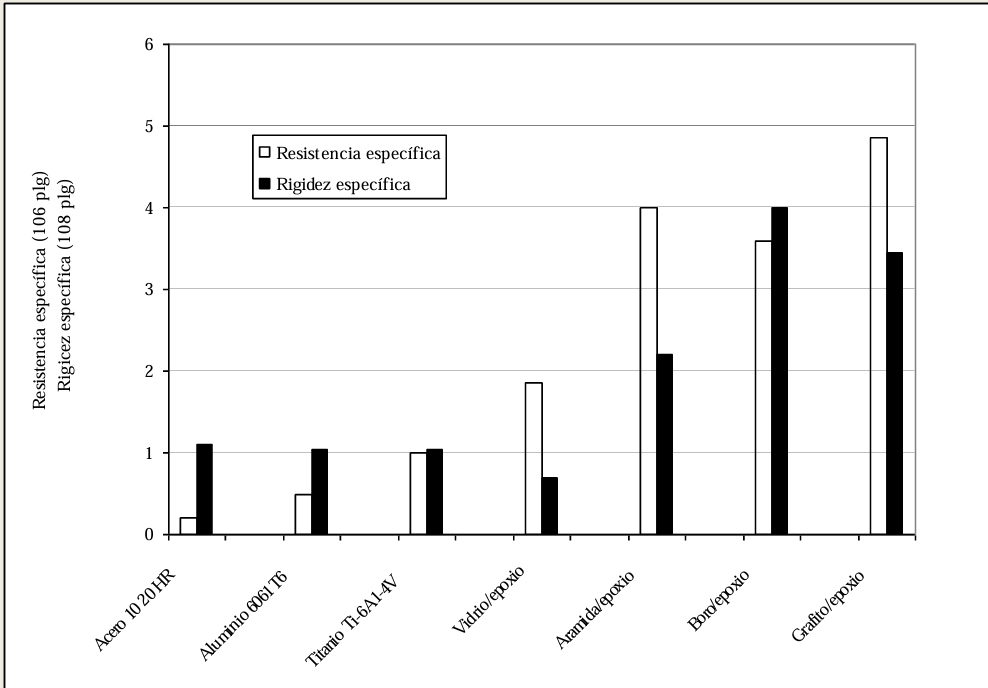
\includegraphics[width=0.4\textwidth]{kevlar.png}
    \caption{Comparativa de resistencia específica y rigidez específica de materiales compuestos y metalicos \\Fuente: diapositivas de la asignatura}
    \label{fig:comparativa_resistencia_rigidez}
\end{figure}

Como puede observarse los primeros muestran mayor resistencia con un menor peso.

\dfn{resistencia especifica}{Resistencia a la traccion dividida por la densidad \\ $\frac{\sigma}{\rho}$}
\dfn{rigidez especifica}{Modulo de Young(elasticidad) dividida por la densidad \\ $\frac{E}{\rho}$}

existen dos tipos de fibra de vidrio, el vidrio E y el vidrio E, La fibra de carbono se obtiene a partir del compuesto orgánico poliacrilonitrilo, mediante el proceso siguiente:
\begin{figure}
    \centering
    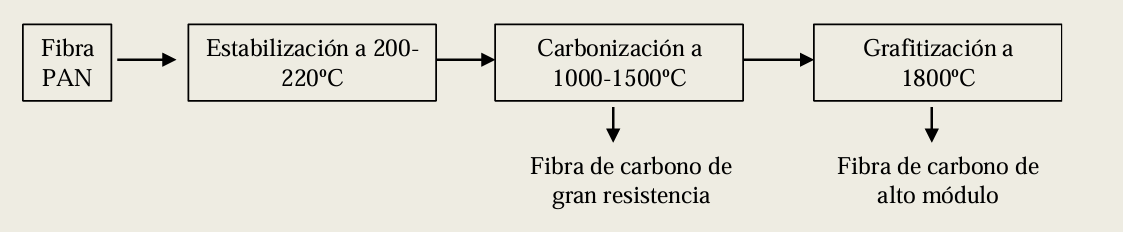
\includegraphics[width=0.4\textwidth]{fibra_de_vidrio.png}
    \caption{Proceso de obtencion de la fibra de vidrio}
    \label{fig:fibra_de_vidrio}
\end{figure}

En primer lugar son estirados y oxidados a temperaturas de 200-220ºC y, tras un proceso de carbonización que elimina O, H y N se produce la grafitización, donde el material sometido a altas temperaturas aumenta el grado de orientación de los cristales tipo grafito dentro de cada fibra.

\nt{Las propiedades mecánicas de los materiales compuestos dependen de su composición siendo asi, intermedias entre las propiedades mecánicas de las fibras y la matriz que forman el material compuesto.}

Por lo general las fibras presentan tensiones de resistencia máxima, límite de proporcionalidad, etc. mucho mayores que las de la matriz que forma el material, presentando el material compuesto un valor intermedio.

\begin{figure}
    \centering
    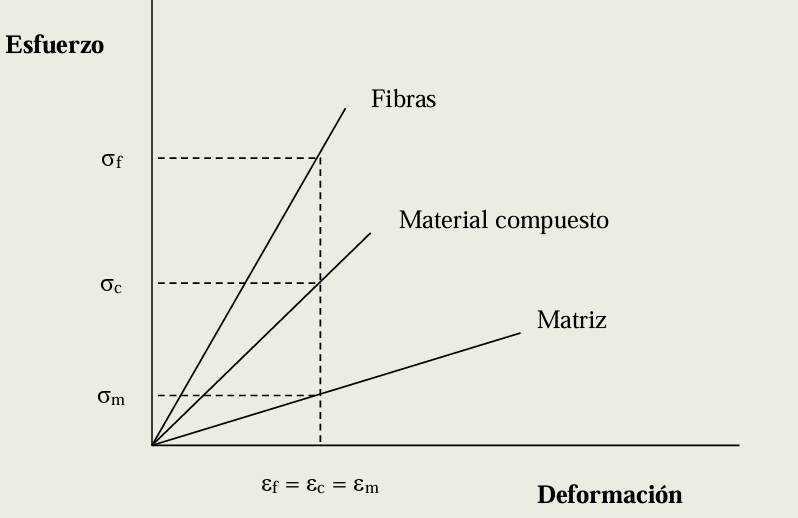
\includegraphics[width=0.4\textwidth]{fibras_vidrio_diagrama_esfuerzo_deformacion.png}
    \caption{Curvas tension-deformacion de materiales compuestos, fibras y matriz \\ Fuente: diapositivas de la asignatura}
    \label{fig:curvas_tension_deformacion}
\end{figure}
Las caracteristicas mas importantes son:
\begin{itemize}
    \item  La \textbf{resistencia máxima a la tracción específica} puede variar hasta cinco veces respecto a las aleaciones de alta resistencia. Los módulos de elasticidad específicos hasta ocho veces.
    \item  Los materiales compuestos pueden funcionar mucho mejor que el acero en aplicaciones donde existen \textbf{cargas cíclicas que produzcan fatiga}.
    \item  Donde se esperen \textbf{cargas de impacto y vibraciones} los materiales compuestos pueden proporcionar un alto nivel de amortiguación.
    \item Como las \textbf{propiedades} de estos materiales \textbf{cambian con la dirección} en las que se colocan las fibras, no son isotropicos, la fabricación de estos materiales se realiza procurando la máxima homogeneidad del material consiguiendo una distribución adecuada de las fibras en el interior del material.
    \item Los \textbf{cambios dimensionales con la temperatura suelen ser menores} en los materiales compuestos que en los metales.
    \item Pueden fabricarse \textbf{estructuras de formas complejas de una sola pieza} lo que reduce el número de operaciones de sujeción, se eliminan las juntas, etc.
\end{itemize}

Aunque estos materiales tienen una serie de \textbf{limitaciones} como son:
\begin{itemize}
    \item \textbf{El coste elevado de las materias primas} de la que están formados.
    \item Su fabricación requiere de \textbf{técnicas más complejas} que las de los materiales convencionales por lo que son distintas y poco generalizadas.
    \item Las \textbf{temperaturas máximas} que pueden soportar los materiales compuestos de matriz polimérica son 260ºC aunque esto puede modificarse con matrices cerámicas o metálicas.
    \item \textbf{Pueden presentar problemas de anisotropía direccional} de sus propiedades \textbf{es decir} que al \textbf{no} ser \textbf{isotrópicas varían con la dirección en la que se aplique la carga}.
    \item El análisis del comportamiento e inspección de estos materiales \textbf{requiere técnicas especiales} que aún no están totalmente desarrolladas.
\end{itemize}
la relacion resistencia coste que hay suele ser mayor en este tipo de materiales.

\subsection{Materiales Semiconductores}
Materiales con \textbf{propiedades de conductividad eléctrica intermedias entre conductores y aislantes fuertemente modulables por dopaje con impurezas atómicas, temperatura o campo eléctrico} (silicio monocristalino, germanio, arseniuro de galio GaAs). Constituyen la base de la instrumentación electrónica, en los \textbf{circuitos integrados} para la industria electrónica y ordenadores. El mas importante de estos es el \textbf{Silicio} puro,
que puede ser modificado para cambiar sus propiedades eléctricas, ya que éstas son extremadamente sensibles a la presencia de átomos de impurezas. También, el germanio, selenio, arseniuro de galio, seleniuro de cinc o teluro de plomo.

\subsection{Tendencia en el uso de materiales y criterios de selección}
los plásticos termoestables pueden utilizarse a temperaturas más altas que los materiales termoplásticos si bien se observa que la temperatura máxima de operación de los distintos materiales termoestables compuestos de matriz polimérica es baja, no superando los 300ºC. Los materiales metálicos son más adecuados cuando se necesitan materiales más resistentes por lo que son los más utilizados en la industria química como componentes fundamentales de las instalaciones.
\section{Aceros, Clasificación y Tratamientos}
\subsection{Sistemas de Clasificación y Nomenclatura (AISI / SAE y UNS)}
Existen organismos internacionales que regulan la nomenclatura de los metales:
\begin{itemize}
    \item \textbf{AISI / SAE:} Clasifica los aceros al carbono y aleados con un código de \textbf{4 dígitos}:
          \begin{itemize}
              \item Los dos primeros dígitos indican los elementos principales de aleación (ej. $10\text{xx}$ para acero al carbono ordinario, $11\text{xx}$ azufre de fácil mecanizado, $41\text{xx}$ cromo-molibdeno, $43\text{xx}$ níquel-cromo-molibdeno).
              \item Los dos últimos dígitos indican el contenido nominal medio de carbono expresado en centésimas de porcentaje (ej. el acero AISI 1020 posee un $0.20\%$ de C; el AISI 1045 un $0.45\%$ de C).
          \end{itemize}
    \item \textbf{Sistema de Numeración Unificada (UNS o SNU):} Código alfanumérico estandarizado por ASTM y SAE compuesto por una letra prefijo y cinco dígitos. Para aceros al carbono se emplea el prefijo \textbf{G} (ej. el AISI 1020 corresponde a UNS G10200). Para aceros inoxidables se emplea el prefijo \textbf{S} (ej. AISI 304 corresponde a UNS S30400).
\end{itemize}
las clasificaciones mas tipicas son la aisi, aa para el aluminio y ASTM
\subsection{Diagrama de Equilibrio Hierro-Carbono (Fe-C)}
Las aleaciones férreas se dividen en función de su porcentaje en masa de carbono:
\begin{itemize}
    \item \textbf{Aceros:} Contenido en carbono inferior al $1.76\%$ (o $2.14\%$ en clasificaciones termodinámicas clásicas).
    \item \textbf{Fundiciones:} Contenido en carbono entre el $2.14\%$ y el $6.67\%$ (límite correspondiente a la formación de cementita pura, $\text{Fe}_3\text{C}$).
\end{itemize}
\nt{lo que quiere es que sepamos que en los aceros de mas de un 6.67\% en carbono no se suele fabricar realmente es mucho mas abajo por que por debajo hay carburo de hierro, en los aceros se considera una aleacion de hierro con carburo de hierro,los que se suelen usar en ingenieria suelen ser de menor de 1.76\% se puede usar de mayor porcentaje que son fundiciones grises por ejemplo para bancos pero al ser demasiado rigidos no son tan utiles en la ingenieria
    para aceros con bajo porcentaje en carbono es ferrita mas carburo de hierro y a mas temperatura ?? si hacemos cambios de temperatura para tratamientos posteriores reducimos las tensiones superficiales pero no cambia la naturaleza}
\subsubsection{Fases y Constituyentes Microestructurales}
\begin{itemize}
    \item \textbf{Ferrita ($\alpha$):} Solución sólida intersticial de carbono en hierro BCC. Es la fase más blanda, dúctil y tenaz del acero (máxima solubilidad de carbono de $0.022\%$ a $727^\circ\text{C}$).
    \item \textbf{Austenita ($\gamma$):} Solución sólida intersticial de carbono en hierro FCC. Estable a alta temperatura (salvo en aceros inoxidables austeníticos estabilizados con Ni a temperatura ambiente). Admite hasta un $2.14\%$ de C disuelto.
    \item \textbf{Cementita ($\text{Fe}_3\text{C}$):} Carburo de hierro intermetálico con $6.67\%$ de C. Es el constituyente más duro ($>60\text{ HRC}$) y quebradizo.
    \item \textbf{Perlita:} Microestructura bifásica laminar formada por láminas alternadas de ferrita y cementita, producto de la descomposición eutectoide de la austenita a $723^\circ\text{C}$ ($0.80\%$ de C).
    \item \textbf{Martensita:} Fase metaestable formada por enfriamiento ultra-rápido (temple) que impide la difusión atómica del carbono, atrapándolo en una estructura tetragonal centrada en el cuerpo (BCT). Presenta extrema dureza pero elevada fragilidad residual.
\end{itemize}

A mayor contenido en carbono (y por consiguiente mayor fracción de cementita y perlita), el acero experimenta un incremento en su resistencia mecánica a la tracción y en su dureza, acompañado por una reducción correlativa de su ductilidad y tenacidad al impacto.

muchas veces no se puede trabajar bien con el material si es demasiado rigido por ello hay que buscar el punto optimo para el trabajo
\subsection{Tipos Principales de Aceros}

\subsubsection{Aceros al Carbono}
\begin{itemize}
    \item \textbf{Bajos en carbono ($\%C < 0.25\%$):} Estructura casi totalmente ferrítica. Muy dúctiles, tenaces, fácilmente conformables en frío y de excelente soldabilidad. Se emplean masivamente en vigas, placas, chapas y tuberías de procesos de baja presión.
    \item \textbf{Medios en carbono ($0.25\% < \%C < 0.60\%$):} Mayor resistencia mecánica y al desgaste. Utilizados en componentes mecánicos sometidos a solicitación dinámica como ejes, árboles de transmisión y engranajes.
    \item \textbf{Altos en carbono ($0.60\% < \%C < 1.40\%$):} Máxima dureza y resistencia, empleados en herramientas de corte, troqueles y resortes.
    \item \textbf{Fundiciones ($\%C > 2.1\%$):} Materiales frágiles con excelente colabilidad y gran amortiguación de vibraciones (utilizadas en bancadas pesadas de maquinaria y carcasas de bombas).
\end{itemize}
/nt{aceros aleados al incluir otras sustancia en general metales para conseguir otros caracter por ejemplo cr para inoxidable wolframio para mayor resistencia mecanica molibdeno y nibio para templabilidad y zonas mas afectadas por la soldadura, vanadio para endurecimiento
acero inoxidable contenido en cromo alto para que sean mas resistentes a la corrosion
}%! Apuntes de clase
\subsubsection{Aceros Inoxidables}
Aleaciones férreas que contienen un mínimo del $10.5\% - 12\%$ de \textbf{cromo}, elemento que reacciona con el oxígeno ambiental formando instantáneamente una capa pasivante nanoscópica de óxido de cromo ($\text{Cr}_2\text{O}_3$) continua, impermeable y autoregenerable que aísla el metal de la corrosión.
\begin{itemize}
    \item \textbf{Martensíticos (Serie AISI 400, ej. 410, 420):} Elevado contenido en carbono. Pueden endurecerse intensamente mediante tratamiento térmico de temple y revenido. Son magnéticos.
    \item \textbf{Ferríticos (Serie AISI 400, ej. 430):} Bajo contenido en carbono y entre $16-18\%$ de Cr. No pueden endurecerse mediante tratamiento térmico. Son magnéticos y se usan en menaje e interiores.
    \item \textbf{Austeníticos (Serie AISI 300, ej. 304, 316):} Los más empleados en la industria química y de procesos. Contienen níquel como estabilizador de la austenita a temperatura ambiente ($18\%\text{ Cr} - 8\%\text{ Ni}$). Son no magnéticos en estado recocido, presentan excelente conformabilidad y tenacidad criogénica extraordinaria.
          \begin{itemize}
              \item \textit{Corrosión por picaduras:} En presencia de cloruros disueltos ($\text{Cl}^-$) el AISI 304 es vulnerable. Para evitarlo se añade entre un $2\%$ y un $3\%$ de \textbf{molibdeno} dando lugar al acero \textbf{AISI 316}.
              \item \textit{Corrosión intergranular y grados bajos en carbono (304L y 316L):} Al calentar o soldar entre $450^\circ\text{C}$ y $850^\circ\text{C}$ precipitan carburos de cromo ($\text{Cr}_{23}\text{C}_6$) en los límites de grano, empobreciendo en cromo las zonas adyacentes y provocando corrosión intergranular. Para evitarlo se recurre a aleaciones de extra-bajo carbono con $\%C \leqslant 0.03\%$ (identificadas con el sufijo \textbf{L}, como el AISI 304L y 316L) o estabilizadas con titanio (AISI 321).
          \end{itemize}
\end{itemize}
%! Apuntes de clase debajo
\nt{Para conseguir ese caracter inoxidable en aceros ya no solo para estructura sino para cierto tipo de maquinaria que va a estar en condiciones muy corrosiva o alimentaria pues serie 400 martensiticos o los ferriticos, los de la serie 300 se suele usar mucho en industria alimentaria serie 304 y 316 los aceros inoxidables son susceptibles a que aparezca corrosion por picadura y se le añade molibdeno}
\subsubsection{Aceros Estructurales ASTM y Perfiles Comerciales}
Estandarizados por la ASTM para edificación y soporte de plantas químicas:
\begin{itemize}
    \item \textbf{ASTM A36:} El acero estructural al carbono más universalmente utilizado ($\sigma_A = 248\text{ MPa}$, $\sigma_M = 400\text{ MPa}$).
    \item \textbf{ASTM A242:} Acero de baja aleación y alta resistencia frente a la corrosión atmosférica a la intemperie (acero tipo \textit{Corten}).
    \item \textbf{ASTM A500 / A501:} Aceros destinados a tubos estructurales conformados en frío y en caliente.
    \item \textbf{ASTM A572:} Acero de alta resistencia de baja aleación al columbio-vanadio (Grados 42, 50, 60 y 65).
\end{itemize}
%! Apuntes de clase debajo
suelen ser parte de equipo angulos barras de sujeccion...  perfiles Hb IBN que son nomenclaturas dependiedo de la forma que tienen.
\textbf{Perfiles estructurales estandarizados más frecuentes:}
\begin{itemize}
    \item \textbf{Perfiles en L (angulares):} Se designan como $\text{L} \, a \times b \times t$ (ej. $\text{L}4 \times 3 \times 1/2$, indicando alas de $4''$ y $3''$ con espesor de $1/2''$).
    \item \textbf{Perfiles en C (canales):} Se designan indicando el peralte y el peso lineal en libras por pie (ej. $\text{C}15 \times 50$, canal de $15''$ de altura y $50\text{ lb/ft}$).
    \item \textbf{Perfiles W (vigas de patín ancho) y S (vigas estándar americanas):} Empleados en vigas principales y columnas resistentes a flexión.
    \item \textbf{Tuberías estructurales cuadradas y rectangulares (HSS):} Gran resistencia bidireccional a torsión y pandeo.
\end{itemize}
%! Apuntes de clase debajo
las vigas de patin ancho se suele usar aunque tenga el mismo material por la forma debido a que la seccion tiene un momento estatico mas elevado, mayor rigidez y soporta mas peso soportan mejor la flexion, tambien comenta un poco lo que son las vigas aligeradas que las tensiones maximas estan en los extremos y por eso se hacen huecos en el centro.
\subsection{Tratamientos de los Aceros}

\subsubsection{Tratamientos Mecánicos}
\begin{itemize}
    \item \textbf{Laminado en caliente (HR - \textit{Hot Rolled}):} Realizado por encima de la temperatura de recristalización. Genera granos equiaxiales libres de tensiones residuales, resultando en un acero blando, dúctil y de menor coste, para reducir espesor o darle mayor resistencia mecanica.
    \item \textbf{Laminado en frío (CR - \textit{Cold Rolled}):} Realizado a temperatura ambiente. Producen acritud intensa, elevando drásticamente el límite elástico y la resistencia a expensas de la ductilidad, con excelentes tolerancias dimensionales,mas severo que en caliente.
    \item \textbf{Estirado en frío (CD - \textit{Cold Drawn}):} Realizado a temperatura ambiente. Producen acritud intensa, elevando drásticamente el límite elástico y la resistencia a expensas de la ductilidad, con excelentes tolerancias dimensionales mas severo que el laminado.
\end{itemize}
%! Apuntes de clase debajo
producir una deformacion plastica para conferir una resistencia mecanica adecuada, al tensar por ejemplo cambia el limite elastico,
el estirado en frio da una resistencia mecanica mayor que los otros, en materiales de misma composicion pero difiriendo el tratamiento mecanico la resistencia sera distinta
\subsubsection{Tratamientos Térmicos}
Modifican la microestructura interna mediante ciclos térmicos controlados de calentamiento, mantenimiento y enfriamiento:
\begin{itemize}
    \item \textbf{Temple y Revenido:} Calentamiento hasta fase austenítica ($800 - 900^\circ\text{C}$) seguido de enfriamiento brusco en agua (WQT) o aceite (OQT) para generar martensita. Dado que la martensita pura es frágil, se aplica inmediatamente un \textbf{revenido} (recalentamiento entre $200^\circ\text{C}$ y $700^\circ\text{C}$) para recuperar tenacidad aliviando tensiones internas.
    \item \textbf{Normalizado:} Calentamiento por encima de la temperatura crítica superior $A_3$ seguido de enfriamiento lento al aire tranquilo. Proporciona grano fino y uniforme, mejorando la maquinabilidad y resistencia al impacto.
    \item \textbf{Recocido completo:} Calentamiento austenítico y enfriamiento extraordinariamente lento dentro del propio horno apagado. Produce la máxima blandura y ductilidad posibles.
    \item \textbf{Recocido de alivio de tensiones:} Calentamiento subcrítico por debajo de $A_1$ ($550 - 650^\circ\text{C}$) para eliminar tensiones residuales derivadas de procesos de soldeo o mecanizado pesado sin alterar la estructura básica del grano.
\end{itemize}
Pretende reducir la dureza debido a que los tratamientos mecanicos generan muchas tensiones residuales, (ejemplo en un vaso si metemos agua hirviendo y hielos continuamente revienta por las tensiones residuales pues esto es lo que se evita con este tratamiento)
calentamiento por debajo de ese limite superior para evitar las tensiones templado, si es mas suave es un normalizado tensiones residuales menores resistencia menor, si se da en el horno se alcnza otras fases por debajo del limite inferior que es un recocido
\subsubsection{Tratamientos Superficiales Termoquímicos}
Incrementan selectivamente la dureza y resistencia al desgaste superficial manteniendo un núcleo interior tenaz y dúctil:
\begin{itemize}
    \item \textbf{Cementación (carburación):} Difusión atómica de carbono en la superficie del acero al calentarlo a $850 - 950^\circ\text{C}$ en atmósfera carburante rica en hidrocarburos ($\text{CH}_4 \rightarrow \text{C} + 2\text{H}_2$), seguido de temple y revenido superficial.
    \item \textbf{Nitruración:} Difusión de nitrógeno atómico a menor temperatura ($500 - 525^\circ\text{C}$) en corriente de amoníaco gas ($2\text{NH}_3 \rightarrow 2\text{N} + 3\text{H}_2$). El nitrógeno precipita formando nitruros duros ($\text{Fe}_4\text{N}$) alcanzando durezas de hasta $80\text{ HRC}$ sin requerir temple posterior.
    \item \textbf{Cianuración:} Formación combinada de carburos y nitruros introduciendo las piezas en un baño de sales fundidas de cianuro a $800 - 900^\circ\text{C}$.
\end{itemize}
pretenden modificar la resistencia de la superficie del metal, por lo general da mayor resistencia a las capas/micras del material, ya que la mayor parte de los fallos del equipo se produce por fatiga qu ees en la superficie del material, se suele tratar la cementacion el acero en alta temperatura se le hace pasar por una corriente de metano para que en la superficie tenga mayor cantidad de carbono (al formarse carburo de hierro en la superficie dando mayor resistencia a la superficie)
con la nitruracion se pretende formar en las micras de la superficie nitruros de hierro a altas temperaturas se pasa amoniaco y reacciona el nitrogeno con el hierro de la superficie aumentando la resistencia mecanicaa y la resis a la corrosion
la cianuracion es cuando se quiere dar ambos Tratamientos

\section{Metodología de Selección de Materiales y Diagramas de Ashby}

La elección final de un material en un proyecto de ingeniería química exige conciliar exigencias multifactoriales: mecánicas (resistencia, rigidez), térmicas, químicas (resistencia a fluidos agresivos), procesabilidad y coste económico.

Para ello se emplea la metodología sistemática propuesta por \textbf{M.~F.~Ashby}, basada en \textbf{diagramas de selección multivariable (Diagramas de Ashby)} que cruzan propiedades contrapuestas en escalas logarítmicas:
\begin{itemize}
    \item Módulo de Young ($E$) frente a densidad ($\rho$) para optimizar componentes con mínima masa y máxima rigidez elástica.
    \item Resistencia mecánica ($\sigma_M$) frente a coste relativo por unidad de volumen.
    \item Empleo de herramientas de software especializado en bases de datos de materiales e índices de mérito (como \textit{Ansys Granta EduPack / CES Selector}).
\end{itemize}
\nt{Para cuando se usa un material para un uso concreto lo mas habitual es ir al fabricante para ese uso concreto aun asi hay usos nuevos donde se necesita elegir el material, hay software y diagramas para seleccionar que tiene en cuenta la densidad y propiedades mecanicas  aunque no entra }


% 3. Problemas resueltos de examen y test de autoevaluación
\clearpage
\section{Problemas Resueltos del Tema 1}

\begin{question}{Módulo de elasticidad a partir de alargamiento en barra recta}{prob:1}
    Una barra recta de sección uniforme está sometida a una fuerza de tracción axial. La sección transversal es de $6\text{ cm}^2$ y la longitud inicial es de $4\text{ m}$. Si el alargamiento total registrado bajo una carga axial de $12\,600\text{ kgf}$ es de $0.40\text{ cm}$, determinar el módulo de elasticidad del material en $\text{kgf}/\text{cm}^2$.
\end{question}

\solve{}
\textbf{1. Datos del problema:}
\begin{itemize}
    \item Sección transversal: $A_0 = 6\text{ cm}^2$
    \item Longitud inicial: $L_0 = 4\text{ m} = 400\text{ cm}$
    \item Carga axial aplicada: $P = 12\,600\text{ kgf}$
    \item Alargamiento elástico total: $\delta = 0.40\text{ cm}$
\end{itemize}

\textbf{2. Ecuaciones fundamentales:}
Asumiendo comportamiento elástico lineal bajo la Ley de Hooke:
\begin{equation*}
    \sigma = E \, \varepsilon \quad \Longleftrightarrow \quad \frac{P}{A_0} = E \, \frac{\delta}{L_0}
\end{equation*}
Despejando el módulo de Young $E$:
\begin{equation*}
    E = \frac{P \cdot L_0}{A_0 \cdot \delta}
\end{equation*}

\textbf{3. Sustitución numérica:}
\begin{equation*}
    E = \frac{12\,600\text{ kgf} \times 400\text{ cm}}{6\text{ cm}^2 \times 0.40\text{ cm}} = \frac{5\,040\,000}{2.4} = 2.10 \times 10^6\text{ kgf}/\text{cm}^2
\end{equation*}
En unidades del Sistema Internacional:
\begin{equation*}
    E \approx 2.10 \times 10^6 \times 9.80665 \times 10^4\text{ Pa} \approx 206\text{ GPa} \quad (\text{correspondiente a un acero})
\end{equation*}


\vspace{1em}

\begin{question}{Compresión uniaxial en cilindro hueco}{prob:2}
    Un cilindro hueco recto de sección circular tiene un diámetro exterior de $7.5\text{ cm}$ y un diámetro interior de $6.0\text{ cm}$. Si se le aplica una fuerza axial de compresión de $5\,000\text{ kgf}$, determinar:
    \begin{enumerate}[label=\alph*)]
        \item La tensión normal de compresión desarrollada.
        \item El acortamiento total que experimenta en una longitud inicial de $50\text{ cm}$.
    \end{enumerate}
    Considérese un módulo de elasticidad $E = 1.05 \times 10^6\text{ kgf}/\text{cm}^2$ y despréciese toda probabilidad de pandeo lateral.
\end{question}

\solve{}
\textbf{1. Datos geométricos y mecánicos:}
\begin{itemize}
    \item Diámetro exterior: $D_{\text{ext}} = 7.5\text{ cm}$
    \item Diámetro interior: $D_{\text{int}} = 6.0\text{ cm}$
    \item Fuerza axial de compresión: $P = 5\,000\text{ kgf}$
    \item Longitud inicial: $L_0 = 50\text{ cm}$
    \item Módulo elástico: $E = 1.05 \times 10^6\text{ kgf}/\text{cm}^2$
\end{itemize}

\textbf{2. Cálculo de la sección transversal neta:}
\begin{equation*}
    A_0 = \frac{\pi}{4} \left(D_{\text{ext}}^2 - D_{\text{int}}^2\right) = \frac{\pi}{4} \left(7.5^2 - 6.0^2\right) = \frac{\pi}{4} (56.25 - 36.00) = \frac{\pi}{4} (20.25) \approx 15.904\text{ cm}^2
\end{equation*}

\textbf{3. Tensión normal de compresión ($\sigma$):}
\begin{equation*}
    \sigma = \frac{P}{A_0} = \frac{5\,000\text{ kgf}}{15.904\text{ cm}^2} \approx 314.38\text{ kgf}/\text{cm}^2 \approx 314.4\text{ kgf}/\text{cm}^2
\end{equation*}

\textbf{4. Acortamiento total elástico ($\delta$):}
Aplicando la relación de Hooke $\sigma = E \, (\delta / L_0)$:
\begin{equation*}
    \delta = \frac{\sigma \cdot L_0}{E} = \frac{314.38\text{ kgf}/\text{cm}^2 \times 50\text{ cm}}{1.05 \times 10^6\text{ kgf}/\text{cm}^2} \approx 0.01497\text{ cm} \approx 0.0150\text{ cm} = 0.15\text{ mm}
\end{equation*}


\vspace{1em}

\begin{question}{Deformación transversal elástica y coeficiente de Poisson en latón}{prob:3}
    Se aplica una carga uniaxial de tracción en la dirección longitudinal de una barra cilíndrica de latón que posee un módulo elástico $E = 10.1 \times 10^4\text{ MPa}$, coeficiente de Poisson $\nu = 0.35$ y un diámetro inicial $d_0 = 10\text{ mm}$. Determinar la magnitud de la carga $P$ necesaria para producir una reducción en el diámetro de $2.5 \times 10^{-3}\text{ mm}$, suponiendo deformación puramente elástica.
\end{question}

\solve{}
\textbf{1. Identificación de magnitudes y datos:}
\begin{itemize}
    \item Módulo de elasticidad: $E = 10.1 \times 10^4\text{ MPa} = 101\,000\text{ N}/\text{mm}^2$
    \item Coeficiente de Poisson: $\nu = 0.35$
    \item Diámetro inicial: $d_0 = 10\text{ mm}$
    \item Variación transversal del diámetro: $\Delta d = -2.5 \times 10^{-3}\text{ mm}$
\end{itemize}

\textbf{2. Deformación unitaria transversal y longitudinal:}
La deformación unitaria lateral en el diámetro es:
\begin{equation*}
    \varepsilon_x = \frac{\Delta d}{d_0} = \frac{-2.5 \times 10^{-3}\text{ mm}}{10\text{ mm}} = -2.5 \times 10^{-4}
\end{equation*}
A partir del coeficiente de Poisson ($\nu = -\varepsilon_x / \varepsilon_z$):
\begin{equation*}
    \varepsilon_z = -\frac{\varepsilon_x}{\nu} = -\frac{-2.5 \times 10^{-4}}{0.35} \approx 7.1429 \times 10^{-4}
\end{equation*}

\textbf{3. Tensión axial requerida ($\sigma_z$):}
Por la ley de Hooke en régimen elástico:
\begin{equation*}
    \sigma_z = E \cdot \varepsilon_z = 101\,000\text{ MPa} \times 7.1429 \times 10^{-4} \approx 72.143\text{ MPa} = 72.143\text{ N}/\text{mm}^2
\end{equation*}

\textbf{4. Cálculo de la carga axial $P$:}
La sección transversal inicial de la probeta es:
\begin{equation*}
    A_0 = \frac{\pi}{4} d_0^2 = \frac{\pi}{4} (10\text{ mm})^2 = 25\pi\text{ mm}^2 \approx 78.54\text{ mm}^2
\end{equation*}
Por tanto, la carga $P$ aplicada resulta:
\begin{equation*}
    P = \sigma_z \cdot A_0 = 72.143\text{ N}/\text{mm}^2 \times 78.54\text{ mm}^2 \approx 5\,666\text{ N} \quad (5.67\text{ kN})
\end{equation*}
\textit{Nota sobre el resultado:} Si el cambio diametral fuese $\Delta d = 2.5 \times 10^{-5}\text{ mm}$, la carga sería $56.66\text{ N}$. Para el valor enunciado en el texto de $2.5 \times 10^{-3}\text{ mm}$, la carga elástica rigurosa es $P = 5\,666\text{ N}$.


\vspace{1em}

\begin{question}{Ductilidad y tensión real de fractura en probeta de acero}{prob:4}
    Una probeta cilíndrica de acero con un diámetro original $d_0 = 12.8\text{ mm}$ se ensaya a tracción uniaxial hasta la fractura, alcanzando una resistencia nominal a la rotura $\sigma_D = 460\text{ MPa}$. Una vez rota la probeta, se mide el diámetro transversal mínimo en la sección de fractura resultando $d_f = 10.7\text{ mm}$. Evaluar:
    \begin{enumerate}[label=\alph*)]
        \item La ductilidad del material expresada mediante el porcentaje de estricción (\%ES).
        \item La tensión real $\sigma_{\text{real}}$ que soportaba la sección de estricción en el instante exacto de la fractura.
    \end{enumerate}
\end{question}

\solve{}
\textbf{1. Datos iniciales y finales:}
\begin{itemize}
    \item Diámetro inicial: $d_0 = 12.8\text{ mm}$
    \item Diámetro final en rotura: $d_f = 10.7\text{ mm}$
    \item Resistencia nominal a rotura: $\sigma_D = 460\text{ MPa} = 460\text{ N}/\text{mm}^2$
\end{itemize}

\textbf{2. Cálculo de áreas transversales inicial y final:}
\begin{align*}
    A_0 & = \frac{\pi}{4} d_0^2 = \frac{\pi}{4} (12.8)^2 \approx 128.68\text{ mm}^2 \\
    A_f & = \frac{\pi}{4} d_f^2 = \frac{\pi}{4} (10.7)^2 \approx 89.92\text{ mm}^2
\end{align*}

\textbf{3. Evaluación del porcentaje de estricción (\%ES):}
\begin{equation*}
    \%ES = \frac{A_0 - A_f}{A_0} \times 100 = \frac{128.68 - 89.92}{128.68} \times 100 = \frac{38.76}{128.68} \times 100 \approx 30.1\% \approx 30\%
\end{equation*}

\textbf{4. Cálculo de la tensión real de fractura ($\sigma_{\text{real}}$):}
La carga total $P_D$ actuante en el momento del colapso se deduce a partir de la tensión nominal de rotura referida al área original:
\begin{equation*}
    P_D = \sigma_D \cdot A_0 = 460\text{ N}/\text{mm}^2 \times 128.68\text{ mm}^2 \approx 59\,192.8\text{ N}
\end{equation*}
La tensión real en la rotura se evalúa dividiendo dicha carga entre la sección transversal final real contraída $A_f$:
\begin{equation*}
    \sigma_{\text{real}} = \frac{P_D}{A_f} = \frac{\sigma_D \cdot A_0}{A_f} = 460 \times \frac{128.68}{89.92} = 460 \times \left(\frac{12.8}{10.7}\right)^2 \approx 460 \times 1.431 \approx 658.2\text{ MPa}
\end{equation*}

\clearpage
\section{Test de Autoevaluación - Tema 1}

\begin{enumerate}[label=\textbf{\arabic*.}]
    \item Los materiales compuestos .....
          \begin{enumerate}[label=\alph*.]
              \item Tienen propiedades homogéneas en todas las direcciones del espacio
              \item \textcolor{red!85!black}{Muestran un buen comportamiento frente a cargas cíclicas.}
              \item Presentan una resistencia específica inferior a la de los metales.
          \end{enumerate}

    \item Si se desea el uso de un material que requiera tener baja densidad y alta flexibilidad, de forma general recurriríamos al uso de un material....
          \begin{enumerate}[label=\alph*.]
              \item Cerámico
              \item \textcolor{red!85!black}{Polimérico termoplástico.}
              \item Polimérico termoestable
          \end{enumerate}

    \item Cuando un material sufre una deformación elástica...
          \begin{enumerate}[label=\alph*.]
              \item \textcolor{red!85!black}{Recupera sus dimensiones al dejar de aplicarse la carga.}
              \item Recupera sus dimensiones siempre que no se haya superado el límite de fluencia o cedencia.
              \item Aumenta su límite de proporcionalidad tras dejar de aplicarse la carga.
          \end{enumerate}

    \item Señale la respuesta correcta:
          \begin{enumerate}[label=\alph*.]
              \item Un mayor valor del módulo de resiliencia indica que el material tiene mayor resistencia a la deformación plástica.
              \item \textcolor{red!85!black}{Un mayor valor del Alargamiento a la rotura y de la Estricción indica que el material es más dúctil.}
              \item Ambas respuestas son correctas
          \end{enumerate}

    \item Señale la respuesta correcta:
          \begin{enumerate}[label=\alph*.]
              \item \textcolor{red!85!black}{El objetivo del ensayo de tracción normalizado permite comparar el comportamiento de materiales entre sí.}
              \item El ensayo tracción-deformación suele mostrar la tensión real que sufre un material en función de su deformación unitaria.
              \item El objetivo del ensayo de tracción normalizado es evaluar el comportamiento que tendrá un material en su uso real.
          \end{enumerate}

    \item Señale la respuesta correcta:
          \begin{enumerate}[label=\alph*.]
              \item \textcolor{red!85!black}{La cianuración es un tratamiento superficial que pretende aumentar la resistencia mecánica de la superficie del acero mediante la inclusión de grupos $\text{CN}^-$ (cianuros) sobre la superficie.}
              \item La nitruración es un tratamiento superficial que pretende aumentar la resistencia mecánica de la superficie del acero mediante la formación de nitratos con base férrea.
              \item La cementación es un tratamiento superficial que pretende aumentar la resistencia mecánica de la superficie del acero mediante la formación de carburo de hierro.
          \end{enumerate}

    \item Señale la respuesta correcta:
          \begin{enumerate}[label=\alph*.]
              \item \textcolor{red!85!black}{Ambas respuestas son correctas}
              \item Un aumento en el contenido en carbono de los aceros los hace menos tenaces.
              \item Un material es más tenaz cuando es capaz de absorber mayor energía plástica y elástica antes de su rotura.
          \end{enumerate}

    \item Los materiales compuestos .....
          \begin{enumerate}[label=\alph*.]
              \item Están formados por un material que le confiere rigidez (fibras) y otro que actúa de relleno.
              \item \textcolor{red!85!black}{Suelen tener una resistencia mecánica intermedia entre las fibras y la matriz}
              \item Ambas respuestas son correctas
          \end{enumerate}

    \item Señale la respuesta correcta:
          \begin{enumerate}[label=\alph*.]
              \item Ambas respuestas son correctas
              \item La tenacidad es la capacidad de un material de absorber energía plástica antes de su fractura.
              \item \textcolor{red!85!black}{La tenacidad se puede evaluar mediante ensayos que miden la energía de impacto de un martillo sobre el material}
          \end{enumerate}

    \item Señale la respuesta correcta:
          \begin{enumerate}[label=\alph*.]
              \item \textcolor{red!85!black}{La deformación plástica aumenta el límite elástico de un material}
              \item La deformación plástica disminuye el límite de proporcionalidad de un material.
              \item La deformación plástica reduce el punto de fluencia de un material
          \end{enumerate}

    \item Señale la respuesta correcta:
          \begin{enumerate}[label=\alph*.]
              \item Un aumento de la carga en el ensayo de termofluencia conlleva una reducción de la mínima rapidez de termofluencia
              \item \textcolor{red!85!black}{La termofluencia conlleva el endurecimiento del material debido a la deformación plástica sufrida.}
              \item La mínima rapidez de termofluencia se produce en las etapas iniciales del ensayo de termofluencia, y nos permitirá evaluar el tiempo de vida que tendría un equipo.
          \end{enumerate}

    \item Señale la respuesta correcta:
          \begin{enumerate}[label=\alph*.]
              \item \textcolor{red!85!black}{El ensayo de Erichsen permite evaluar la capacidad que tiene un material plano de ser transformado en piezas huecas como fondos, carcasas, etc.}
              \item El ensayo de flexibilidad permite evaluar las propiedades mecánicas de resistencia que tiene un material.
              \item Dentro de los ensayos no destructivos podemos encontrar el ensayo de dureza Rockwell superficial
          \end{enumerate}

    \item Señale la respuesta correcta:
          \begin{enumerate}[label=\alph*.]
              \item El límite de proporcionalidad y el límite de elasticidad siempre coinciden.
              \item \textcolor{red!85!black}{El límite de fluencia inferior es un punto característico del material}
              \item Ambas respuestas son correctas
          \end{enumerate}

    \item En cuanto a la resistencia por fatiga que tienen los materiales
          \begin{enumerate}[label=\alph*.]
              \item La resistencia a la fatiga dependerá de la resistencia mecánica propia que tenga el material, pero no del ambiente de trabajo en el que desarrolle su labor.
              \item \textcolor{red!85!black}{Superficies más pulidas conllevarán mayor resistencia a la fatiga.}
              \item Los procesos superficiales de carburación, nitruración, etc. no mejora la resistencia a la fatiga del material ya que la resistencia mecánica del material completo sigue siendo la misma.
          \end{enumerate}

    \item La tensión ingenieril se define como:
          \begin{enumerate}[label=\alph*.]
              \item Ambas son incorrectas
              \item \textcolor{red!85!black}{Cociente entre la carga aplicada y la sección (inicial) del material transversal a la dirección de aplicación de la carga.}
              \item Cociente entre la carga aplicada y la sección (en cada momento del ensayo) del material transversal a la dirección de aplicación de la carga.
          \end{enumerate}

    \item Señale la respuesta correcta:
          \begin{enumerate}[label=\alph*.]
              \item Un aumento de la temperatura hace que generalmente los materiales sean más rígidos.
              \item \textcolor{red!85!black}{Los ensayos de termofluencia permiten evaluar el comportamiento de un material frente a temperaturas y cargas elevadas en función del tiempo.}
              \item Ambas respuestas son correctas
          \end{enumerate}

    \item Señale la respuesta correcta:
          \begin{enumerate}[label=\alph*.]
              \item El laminado del acero tiene como objetivo la reducción del espesor de la plancha de metal
              \item \textcolor{red!85!black}{El carácter inoxidable de un acero se lo da el contenido en cromo en la aleación, que suele estar entre en una proporción de 10-27\%.}
              \item Uno de los aceros inoxidables más utilizados en la industria alimentaria es el AISI 9228.
          \end{enumerate}

    \item Señale la respuesta correcta:
          \begin{enumerate}[label=\alph*.]
              \item La deformación unitaria se define como el cociente entre el alargamiento y la longitud inicial de la probeta
              \item \textcolor{red!85!black}{Ambas son correctas}
              \item El alargamiento o deformación se define como la elongación que sufre un material en la dirección de aplicación de la carga
          \end{enumerate}

    \item Señale la respuesta correcta:
          \begin{enumerate}[label=\alph*.]
              \item La resistencia máxima a la tracción es el punto donde la tensión real aplicada es máxima
              \item Ambas respuestas son correctas
              \item \textcolor{red!85!black}{En caso de que el límite de fluencia no esté claro, se puede definir como la tensión para la cual la deformación plástica es del 0.2\%.}
          \end{enumerate}

    \item Señale la respuesta correcta:
          \begin{enumerate}[label=\alph*.]
              \item Un aumento de la temperatura en el ensayo de termofluencia conlleva una reducción de la mínima rapidez de termofluencia
              \item La fluencia lenta o termofluencia es mayor en las etapas iniciales del ensayo
              \item \textcolor{red!85!black}{La mínima rapidez de termofluencia nos muestra el crecimiento exponencial de la deformación que sufre un material.}
          \end{enumerate}

    \item Si se desea el uso de un material que requiera tener alta dureza, resistencia al desgaste y con propiedades aislantes y térmicas, de forma general recurriríamos al uso de un material....
          \begin{enumerate}[label=\alph*.]
              \item Polimérico
              \item Metálico
              \item \textcolor{red!85!black}{Cerámico}
          \end{enumerate}

    \item Señale la respuesta correcta:
          \begin{enumerate}[label=\alph*.]
              \item La tensión de trabajo coincide con la tensión en el punto de fluencia o con la resistencia máxima a la tracción, seleccionándose uno de estos valores en función de las condiciones de servicio del material.
              \item \textcolor{red!85!black}{La tensión de seguridad o tensión de trabajo es la tensión máxima que puede soportar un material en sus condiciones de servicio.}
              \item El producto de la tensión en el punto de fluencia o en el punto de máxima tracción (dependiendo del material y uso del mismo) por el coeficiente de seguridad nos determinará la tensión de trabajo del material.
          \end{enumerate}

    \item El acero es una aleación hierro-carbono donde.....
          \begin{enumerate}[label=\alph*.]
              \item Cuanto mayor porcentaje en carbono mayor presente, mayor resistencia mecánica tendrá el material
              \item \textcolor{red!85!black}{Ambas respuestas son correctas}
              \item La ferrita es hierro casi puro y la cementita es un carburo de hierro
          \end{enumerate}

    \item Señale la respuesta correcta:
          \begin{enumerate}[label=\alph*.]
              \item Ambas respuestas son correctas
              \item \textcolor{red!85!black}{La ductilidad es una medida de la deformación plástica que sufre un material antes de su fractura.}
              \item La tenacidad es una medida de la deformación elástica que sufre un material antes de su fractura.
          \end{enumerate}

    \item Señale la respuesta correcta:
          \begin{enumerate}[label=\alph*.]
              \item \textcolor{red!85!black}{Los tratamientos mecánicos tienen como objetivo producir una deformación plástica en el material para conferir una resistencia determinada.}
              \item Un enfriamiento rápido del material desde la temperatura crítica máxima tiene como objetivo reducir las tensiones residuales que aparecen en el material tras un proceso térmico más severo.
              \item Los tratamientos superficiales aplicados a aceros pretenden dar al material una mayor resistencia mecánica al material debido a la deformación plástica que sufre la superficie.
          \end{enumerate}

    \item Ensayo de microdureza:
          \begin{enumerate}[label=\alph*.]
              \item \textcolor{red!85!black}{Vickers y Knoop}
          \end{enumerate}
\end{enumerate}



\chapter{Resistencia Química de Materiales. Corrosión}

\section{Introducción y Relevancia en la Ingeniería Química}

La \textbf{corrosión} es un fenómeno natural y espontáneo por medio del cual los sistemas químicos manifiestan su tendencia termodinámica hacia un estado de equilibrio de menor energía libre. En el ámbito de los materiales y la ingeniería de procesos, se define como:

\dfn{Corrosión}{Reacción química o electroquímica entre un material (principalmente metálico) y su entorno o medio de contacto, que provoca el deterioro progresivo de sus propiedades físicas, químicas y mecánicas.}

La mayor parte de los procesos de corrosión se manifiestan en los materiales metálicos, efectuándose este ataque mediante mecanismos \textbf{electroquímicos} (en presencia de un electrolito) o por \textbf{ataque químico directo} (especialmente a temperaturas elevadas o en medios no polares). 

Sin embargo, los materiales no metálicos también experimentan procesos de degradación química directa:
\begin{itemize}
    \item \textbf{Materiales cerámicos y refractarios:} No sufren corrosión electroquímica al no poseer electrones libres de conducción, pero son atacados químicamente por sales fundidas a elevadas temperaturas, medios fuertemente básicos y ácidos específicos como el ácido fluorhídrico ($\text{HF}$).
    \item \textbf{Polímeros y elastómeros:} No sufren corrosión electroquímica; su deterioro se denomina \textbf{degradación}, producida por absorción de agua, disolventes orgánicos (hinchamiento y disolución) o por escisión de cadenas macromoleculares ante la acción combinada de radiación ultravioleta (UV) y oxígeno (por ejemplo, fragilización del PVC expuesto a la intemperie).
\end{itemize}

\nt{En la industria química, los materiales resistentes a la corrosión suelen presentar costes muy elevados o baja resistencia a las cargas mecánicas. Por tanto, el diseño de equipos implica un compromiso técnico-económico: seleccionar un material resistente mecánicamente (como aceros al carbono o de baja aleación) y prever un sobreespesor por corrosión (\textit{corrosion allowance}), o aplicar recubrimientos y métodos de protección adecuados.}

\subsection{Impacto socioeconómico de la corrosión}
El estudio de la corrosión abarca dimensiones económicas, de seguridad técnica y medioambientales:
\begin{itemize}
    \item \textbf{Impacto en el PIB:} Las pérdidas anuales causadas por corrosión en países industrializados y en vías de desarrollo se estiman en torno al \textbf{3.5\% del Producto Interior Bruto (PIB)}.
    \item \textbf{Consumo de recursos:} Entre \textbf{1/4 y 1/3 de la producción mundial de acero} se destina exclusivamente a la reposición de componentes e infraestructuras metálicas deterioradas.
\end{itemize}

\begin{figure}[H]
    \centering
    \begin{tikzpicture}[node distance=2.5cm, auto, >=Latex]
        \node [draw, rectangle, rounded corners, fill=blue!10, text width=5cm, align=center, thick] (mineral) {\textbf{Metales en la Naturaleza}\\(Óxidos, hidróxidos, sales)\\\textit{Compuestos de baja energía / Estables}};
        \node [draw, rectangle, rounded corners, fill=red!10, text width=5cm, align=center, thick, below of=mineral, yshift=-1cm] (puro) {\textbf{Metales Puros / Aleaciones}\\(Estado metaestable)\\\textit{Mayor contenido energético}};
        
        \draw [->, line width=1.5pt, blue!70!black] (mineral) -- node[midway, right, align=left] {\textbf{Metalurgia Extractiva}\\(Aporte de energía / Reducción)} (puro);
        \draw [->, line width=1.5pt, red!70!black] ([xshift=-1.5cm]puro.north) -- node[midway, left, align=right] {\textbf{Corrosión}\\(Proceso espontáneo $\Delta G < 0$)\\(Retorno al estado combinado)} ([xshift=-1.5cm]mineral.south);
    \end{tikzpicture}
    \caption{Ciclo metalúrgico y naturaleza termodinámica de la corrosión.}
    \label{fig:ciclo_corrosion}
\end{figure}

\subsection{Pérdidas económicas por corrosión}
Las pérdidas económicas provocadas por la corrosión se clasifican en:
\begin{enumerate}
    \item \textbf{Pérdidas directas:}
          \begin{itemize}
              \item Reposición y sustitución de maquinaria, tuberías, válvulas y estructuras colapsadas.
              \item Aplicación periódica de pinturas, revestimientos e inhibidores químicos.
              \item Sobrecoste por el empleo de aleaciones especiales de alta gama (aceros inoxidables austeníticos, titanio, inconel, hastelloys).
          \end{itemize}
    \item \textbf{Pérdidas indirectas:}
          \begin{itemize}
              \item \textbf{Paradas de planta no programadas:} Lucro cesante e interrupción del proceso productivo para reparar fugas o sustituir elementos críticos.
              \item \textbf{Pérdidas de producto y fugas:} Fugas en conducciones y tanques presurizados, con riesgo añadido de contaminación y explosiones.
              \item \textbf{Pérdidas de eficiencia y rendimiento térmico:} Acumulación de costras de óxido e incrustaciones en tubos de intercambiadores de calor, reduciendo drásticamente el coeficiente global de transmisión de calor ($U$).
              \item \textbf{Sobredimensionamiento de equipos:} Incremento excesivo de espesores de pared por desconocimiento o incertidumbre en las velocidades reales de corrosión.
          \end{itemize}
\end{enumerate}

%=============================================================================
\section{Ensayos de Corrosión}

Los objetivos fundamentales de los ensayos de corrosión en ingeniería son:
\begin{itemize}
    \item Seleccionar el material idóneo para una aplicación de proceso concreta.
    \item Evaluar el comportamiento de nuevos materiales y recubrimientos en condiciones límite de operación.
    \item Determinar la agresividad de reactivos, productos intermedios y contaminantes en planta.
    \item Investigar y modelizar los mecanismos cinéticos y electroquímicos de degradación.
\end{itemize}

\subsection{Clasificación de los ensayos de corrosión}
Para que los resultados sean reproducibles, comparables y fiables, los ensayos deben estar estrictamente normalizados según organismos internacionales como la \textbf{NACE} (\textit{National Association of Corrosion Engineers}), la \textbf{ASTM} y el \textbf{MTI} (\textit{Materials Technology Institute}).

\begin{enumerate}
    \item \textbf{Ensayos de laboratorio:} Realizados sobre probetas estandarizadas a pequeña escala bajo condiciones controladas (temperatura, concentración, pH, agitación). Su objetivo principal es el \textbf{cribado previo y descarte} de materiales inadecuados.
    \item \textbf{Ensayos en planta piloto:} Son los más representativos y deseables antes de la construcción industrial, ya que reproducen de forma fidedigna los gradientes térmicos reales, velocidades de flujo, impurezas de materias primas y relaciones área/volumen de la instalación definitiva.
    \item \textbf{Ensayos en planta en servicio:} Técnicas de monitorización \textit{in situ} sobre equipos reales en operación mediante cupones de corrosión, sondas de resistencia eléctrica o ensayos no destructivos (ultrasonidos, corrientes inducidas, radiografía).
\end{enumerate}

\subsection{Variables experimentales que influyen en el ensayo}
\begin{itemize}
    \item \textbf{Caracterización de la muestra:} Composición química exacta, tratamiento térmico previo, tamaño de grano y microestructura. Probetas de referencia archivadas y perfectamente trazables.
    \item \textbf{Preparación superficial:} Superficie pulida y desengrasada. El acabado pulido estandarizado minimiza la rugosidad; para trasladar datos a escala real debe emplearse un \textbf{factor de corrección de laboratorio} (que puede variar de 1 a 10).
    \item \textbf{Técnicas de fijación y exposición:} Las probetas deben sumergirse totalmente aisladas de soportes metálicos mediante materiales plásticos o cerámicos (teflón) para evitar la formación espuria de pilas galvánicas.
    \item \textbf{Tiempo de ensayo:} La velocidad de corrosión suele ser elevada en las fases iniciales y decrecer conforme se forman productos de corrosión. Generalmente se realizan ensayos en \textbf{5 períodos de 48 horas}, renovando la disolución corrosiva en cada ciclo. De forma empírica, el tiempo mínimo de ensayo se evalúa mediante:
          \begin{equation}
              t_{\text{mínimo}} \text{ [horas]} = \frac{2000}{\text{velocidad de corrosión esperada [mpy]}}
              \label{eq:tiempo_minimo_ensayo}
          \end{equation}
    \item \textbf{Aireación:} La presencia de oxígeno disuelto incrementa sensiblemente la corrosión en aceros al carbono, mientras que favorece la pasivación protectora en aluminio y aceros inoxidables. Los ensayos con aireación se realizan burbujeando aire u oxígeno, y los ensayos desaireados burbujeando nitrógeno gaseoso inerte.
    \item \textbf{Limpieza post-ensayo:} Eliminación estricta de productos de corrosión sin desgastar el metal base no atacado mediante limpieza mecánica (cepillos suaves/abrasivos ligeros), química (disolventes/decapantes inhibidos) o electrolítica (polarización catódica de la probeta).
    \item \textbf{Temperatura:} Es una de las variables más críticas. Por regla general, un incremento de temperatura acelera exponencialmente la corrosión (cinética tipo Arrhenius), salvo cuando promueve la formación de fases pasivantes estables o cuando disminuye la solubilidad del oxígeno en líquidos acuosos abiertos (el agua fría abierta retiene más $O_2$ disuelto y puede ser más corrosiva que el agua caliente desoxigenada).
\end{itemize}

\begin{table}[H]
    \centering
    \caption{Efecto de la temperatura en la corrosión del acero inoxidable 18-8S en ácido nítrico al 65\%.}
    \begin{tabular}{cc}
        \toprule
        \textbf{Temperatura ($^\circ$F)} & \textbf{Velocidad de corrosión (mpy)} \\
        \midrule
        Hasta 250 & $< 20$ \\
        260 & 100 \\
        280 & 200 \\
        320 & 500 \\
        330 & 1000 \\
        370 & 5000 \\
        \bottomrule
    \end{tabular}
    \label{tab:efecto_temp_hno3}
\end{table}

\subsection{Expresión cuantitativa y unidades de la velocidad de corrosión}
La velocidad de corrosión uniforme se cuantifica a través de la pérdida de masa por unidad de área y tiempo, traduciéndose a una \textbf{pérdida de espesor por penetración}:

\dfn{Milipulgadas por año (mpy)}{Pérdida de espesor lineal expresada en milésimas de pulgada ($1\text{ mil} = 10^{-3}\text{ in} = 0.0254\text{ mm}$) por año de exposición continua:}
\begin{equation}
    \text{mpy} = \frac{534 \cdot W}{D \cdot A \cdot T}
    \label{eq:mpy_formula}
\end{equation}
donde $W$ es la pérdida de masa en $\text{mg}$, $D$ la densidad del material en $\text{g/cm}^3$, $A$ el área expuesta en $\text{in}^2$ y $T$ el tiempo de ensayo en $\text{horas}$.

En unidades del Sistema Internacional (SI) y normas europeas se emplea la tasa de penetración en $\text{mm/año}$:
\begin{equation}
    \text{Velocidad de penetración } \left[\frac{\text{mm}}{\text{año}}\right] = \frac{87.6 \cdot W}{D \cdot A \cdot T}
    \label{eq:mm_year_formula}
\end{equation}
donde $W$ está en $\text{mg}$, $D$ en $\text{g/cm}^3$, $A$ en $\text{cm}^2$ y $T$ en $\text{horas}$.

\textbf{Factores de conversión de unidades de velocidad de corrosión:}
\begin{equation}
    1\text{ mpy} = 0.0254\text{ }\frac{\text{mm}}{\text{año}} = 25.4\text{ }\frac{\mu\text{m}}{\text{año}} = 2.90\text{ }\frac{\text{nm}}{\text{h}} = 0.805\text{ }\frac{\text{pm}}{\text{s}}
    \label{eq:conversion_corrosion}
\end{equation}

\begin{table}[H]
    \centering
    \caption{Calificación relativa de materiales frente a su resistencia a la corrosión uniforme.}
    \begin{tabular}{lccccc}
        \toprule
        \textbf{Resistencia Relativa} & \textbf{mpy} & \textbf{mm/año} & \textbf{$\mu$m/año} & \textbf{nm/h} & \textbf{pm/s} \\
        \midrule
        \textbf{Excepcional} & $< 1$ & $< 0.02$ & $< 25$ & $< 2$ & $< 1$ \\
        \textbf{Excelente} & $1 - 5$ & $0.02 - 0.1$ & $25 - 100$ & $2 - 10$ & $1 - 5$ \\
        \textbf{Bueno} & $5 - 20$ & $0.1 - 0.5$ & $100 - 500$ & $10 - 50$ & $5 - 20$ \\
        \textbf{Razonable} & $20 - 50$ & $0.5 - 1.0$ & $500 - 1000$ & $50 - 150$ & $20 - 50$ \\
        \textbf{Pobre} & $50 - 200$ & $1.0 - 5.0$ & $1000 - 5000$ & $150 - 500$ & $50 - 200$ \\
        \textbf{Inaceptable} & $> 200$ & $> 5.0$ & $> 5000$ & $> 500$ & $> 200$ \\
        \bottomrule
    \end{tabular}
    \label{tab:clasificacion_resistencia}
\end{table}

%=============================================================================
\section{Fundamentos Termodinámicos y Electroquímicos de la Corrosión}

\subsection{Criterio termodinámico de espontaneidad ($\Delta G$)}
La viabilidad termodinámica de un proceso de corrosión viene determinada por la variación de la \textbf{energía libre de Gibbs} ($\Delta G$). Para una reacción química o electroquímica:
\begin{equation}
    \Delta G = \sum G_{\text{productos}} - \sum G_{\text{reactivos}}
\end{equation}
\begin{itemize}
    \item $\Delta G < 0$: Proceso termodinámicamente espontáneo (tendencia natural a corroerse).
    \item $\Delta G > 0$: Proceso no espontáneo en las condiciones dadas (inmunidad termodinámica).
    \item $\Delta G = 0$: Estado de equilibrio termodinámico.
\end{itemize}

\textbf{Ejemplos termodinámicos de corrosión en medio húmedo con oxígeno:}
\begin{align}
    \text{Mg} + \text{H}_2\text{O} + \frac{1}{2}\text{O}_2 &\longrightarrow \text{Mg(OH)}_2 & \Delta G^\circ &= -142\,600\text{ cal} \quad (\text{Espontánea, alta reactividad}) \\
    \text{Cu} + \text{H}_2\text{O} + \frac{1}{2}\text{O}_2 &\longrightarrow \text{Cu(OH)}_2 & \Delta G^\circ &= -28\,600\text{ cal} \quad (\text{Espontánea, reactividad moderada}) \\
    \text{Au} + \frac{3}{2}\text{H}_2\text{O} + \frac{3}{4}\text{O}_2 &\longrightarrow \text{Au(OH)}_3 & \Delta G^\circ &= +15\,700\text{ cal} \quad (\text{No espontánea, metal noble inmune})
\end{align}

\nt{La energía libre de Gibbs $\Delta G$ indica únicamente la tendencia termodinámica de la reacción, pero \textbf{no predice en absoluto la velocidad con la que se producirá el ataque}. Metales con una $\Delta G$ fuertemente negativa (como el aluminio o el titanio) pueden reaccionar con extrema lentitud debido a la formación instantánea de películas pasivantes de óxido de alta adherencia que bloquean la difusión de reactivos.}

\subsection{Cinética y energía de activación ($Q_0$)}
Para que la reacción tenga lugar es necesario superar una barrera energética o \textbf{energía de activación} ($Q_0$). La constante cinética de velocidad de reacción sigue la ley de Arrhenius:
\begin{equation}
    k = A \cdot e^{-\frac{Q_0}{R \cdot T}}
    \label{eq:arrhenius}
\end{equation}
donde $A$ es el factor preexponencial de frecuencia, $R = 8.314\text{ J/(mol}\cdot\text{K)}$ la constante universal de los gases y $T$ la temperatura absoluta en Kelvin.

\subsection{Naturaleza electroquímica: Semirreacciones redox}
Toda reacción de corrosión en medio húmedo es un proceso electroquímico acoplado que involucra simultáneamente:
\begin{enumerate}
    \item \textbf{Reacción anódica (Oxidación):} Los átomos metálicos ceden electrones y pasan al electrolito como cationes solvatados. Tiene lugar en las regiones superficiales denominadas \textbf{ánodos}:
          \begin{equation}
              \text{M} \longrightarrow \text{M}^{n+} + n\,e^-
          \end{equation}
    \item \textbf{Reacción catódica (Reducción):} Una especie química presente en el electrolito consume los electrones cedidos por el metal en las zonas superficiales denominadas \textbf{cátodos}:
          \begin{equation}
              \text{Oxidante} + n\,e^- \longrightarrow \text{Reductor}
          \end{equation}
\end{enumerate}

\imp{Por el principio de conservación de la carga y electroneutralidad, \textbf{la velocidad total de oxidación debe ser idéntica a la velocidad total de reducción} en todo instante:
\begin{equation*}
    I_{\text{anódica}} = I_{\text{catódica}} \implies \sum v_{\text{oxidación}} = \sum v_{\text{reducción}}
\end{equation*}}

\subsection{Ecuación de Nernst}
La relación fundamental entre la energía libre de Gibbs y el potencial reversible de celda ($E$) viene dada por:
\begin{equation}
    \Delta G = -n \cdot F \cdot E, \qquad \Delta G^\circ = -n \cdot F \cdot E^\circ
\end{equation}
donde $n$ es el número de electrones transferidos y $F = 96\,485\text{ C/mol} \approx 96\,500\text{ C/mol}$ es la constante de Faraday.

Para una reacción redox general del tipo $a\text{A} + b\text{B} \longleftrightarrow p\text{P} + q\text{Q}$:
\begin{equation}
    E = E^\circ - \frac{R \cdot T}{n \cdot F} \ln \left( \frac{[\text{P}]^p [\text{Q}]^q}{[\text{A}]^a [\text{B}]^b} \right)
    \label{eq:nernst_general}
\end{equation}
A condiciones estándar de temperatura y presión ($T = 298.15\text{ K} = 25^\circ\text{C}$, $1\text{ atm}$), empleando el logaritmo decimal:
\begin{equation}
    E = E^\circ - \frac{0.0592}{n} \log \left( \frac{[\text{P}]^p [\text{Q}]^q}{[\text{A}]^a [\text{B}]^b} \right)
    \label{eq:nernst_25C}
\end{equation}

Para un electrodo metálico puro sumergido en una disolución de sus propios iones ($\text{Me}^{n+} + n\,e^- \longleftrightarrow \text{Me}$), el potencial de reducción reversible es:
\begin{equation}
    E = E^\circ + \frac{0.0592}{n} \log [\text{Me}^{n+}]
    \label{eq:nernst_metal}
\end{equation}

\subsection{Serie electroquímica de potenciales estándar}
Tomando como referencia arbitraria cero el \textbf{Electrodo Estándar de Hidrógeno (EEH)}:
\begin{equation}
    2\text{H}^+ + 2\,e^- \longleftrightarrow \text{H}_2(g) \qquad (E^\circ = 0.000\text{ V})
\end{equation}

\begin{table}[H]
    \centering
    \caption{Potenciales estándar de reducción ($E^\circ$) a 25$^\circ$C.}
    \begin{tabular}{lcr}
        \toprule
        \textbf{Carácter} & \textbf{Semirreacción catódica} & \textbf{$E^\circ$ (V)} \\
        \midrule
        \multirow{5}{*}{\parbox{3cm}{\centering \textbf{Catódicos / Nobles}\\(Inactividad creciente)}} 
        & $\text{Au}^{3+} + 3\,e^- \longrightarrow \text{Au}$ & $+1.420$ \\
        & $\text{O}_2 + 4\text{H}^+ + 4\,e^- \longrightarrow 2\text{H}_2\text{O}$ & $+1.229$ \\
        & $\text{Fe}^{3+} + e^- \longrightarrow \text{Fe}^{2+}$ & $+0.771$ \\
        & $\text{O}_2 + 2\text{H}_2\text{O} + 4\,e^- \longrightarrow 4\text{OH}^-$ & $+0.401$ \\
        & $\text{Cu}^{2+} + 2\,e^- \longrightarrow \text{Cu}$ & $+0.337$ \\
        \midrule
        \textbf{Referencia} & $2\text{H}^+ + 2\,e^- \longrightarrow \text{H}_2(g)$ & $0.000$ \\
        \midrule
        \multirow{5}{*}{\parbox{3cm}{\centering \textbf{Anódicos / Activos}\\(Actividad creciente)}} 
        & $\text{Pb}^{2+} + 2\,e^- \longrightarrow \text{Pb}$ & $-0.126$ \\
        & $\text{Sn}^{2+} + 2\,e^- \longrightarrow \text{Sn}$ & $-0.136$ \\
        & $\text{Ni}^{2+} + 2\,e^- \longrightarrow \text{Ni}$ & $-0.250$ \\
        & $\text{Fe}^{2+} + 2\,e^- \longrightarrow \text{Fe}$ & $-0.440$ \\
        & $\text{Zn}^{2+} + 2\,e^- \longrightarrow \text{Zn}$ & $-0.763$ \\
        & $\text{Al}^{3+} + 3\,e^- \longrightarrow \text{Al}$ & $-1.662$ \\
        \bottomrule
    \end{tabular}
    \label{tab:potenciales_estandar}
\end{table}

\nt{Los elementos con $E^\circ < 0$ son más activos (anódicos) que el hidrógeno y tienden a oxidarse espontáneamente desprendiendo hidrógeno en disoluciones ácidas libres de oxidantes. Los elementos situados más arriba en la tabla tienden a actuar como cátodos y reducirse, mientras que los situados más abajo se oxidan.}

%=============================================================================
\section{Pilas Galvánicas Responsables de la Corrosión}

La corrosión electroquímica requiere la coexistencia de zonas anódicas y zonas catódicas en contacto eléctrico e inmersas en un electrolito conductor. Los tipos de pilas que originan corrosión en la industria son:

\subsection{Pilas galvánicas de dos metales disímiles}
Formadas por dos metales distintos conectados eléctricamente y sumergidos en un electrolito. El metal con potencial de electrodo más electronegativo actúa como ánodo y se corroe aceleradamente.

\ex{Cálculo de la FEM en una pila Zn-Ni}{
Una cuba electrolítica a 25$^\circ$C consta de un electrodo de zinc sumergido en $\text{ZnSO}_4$ $0.1\text{ M}$ ($E^\circ_{\text{Zn}^{2+}/\text{Zn}} = -0.763\text{ V}$) y un electrodo de níquel en $\text{NiSO}_4$ $0.05\text{ M}$ ($E^\circ_{\text{Ni}^{2+}/\text{Ni}} = -0.250\text{ V}$), separados por membrana porosa. Determinar el potencial de la celda.

\textbf{Solución:}
Al comparar potenciales, el $\text{Zn}$ es más electronegativo, actuando como ánodo:
\begin{align*}
    \text{Ánodo (Oxidación):} & \quad \text{Zn} \longrightarrow \text{Zn}^{2+} + 2\,e^- \quad (E^\circ_{\text{ox}} = +0.763\text{ V}) \\
    \text{Cátodo (Reducción):} & \quad \text{Ni}^{2+} + 2\,e^- \longrightarrow \text{Ni} \quad (E^\circ_{\text{red}} = -0.250\text{ V}) \\
    \text{Reacción global:} & \quad \text{Zn} + \text{Ni}^{2+} \longrightarrow \text{Zn}^{2+} + \text{Ni} \quad (E^\circ_{\text{celda}} = 0.763 - 0.250 = +0.513\text{ V})
\end{align*}
Aplicando la ecuación de Nernst:
\begin{equation*}
    E = E^\circ_{\text{celda}} - \frac{0.0592}{2} \log \left( \frac{[\text{Zn}^{2+}]}{[\text{Ni}^{2+}]} \right) = 0.513 - \frac{0.0592}{2} \log \left( \frac{0.1}{0.05} \right) = 0.513 - 0.0296 \log(2) \approx \mathbf{0.504\text{ V}}
\end{equation*}
Al ser $E > 0$, la reacción transcurre espontáneamente con disolución anódica del zinc.
}

\subsection{Reacciones catódicas habituales en medios acuosos}
\begin{table}[H]
    \centering
    \caption{Principales reacciones catódicas según el pH y la presencia de oxidantes.}
    \begin{tabular}{llc}
        \toprule
        \textbf{Tipo de Reacción} & \textbf{Ecuación Química Catódica} & \textbf{$E^\circ$ (V)} \\
        \midrule
        \textbf{1. Deposición metálica} & $\text{M}^{n+} + n\,e^- \longrightarrow \text{M}$ (ej. $\text{Cu}^{2+} + 2e^- \rightarrow \text{Cu}$) & Variable \\
        \textbf{2. Desprendimiento de $\text{H}_2$ (medio ácido)} & $2\text{H}^+ + 2\,e^- \longrightarrow \text{H}_2(g)$ & $0.000$ \\
        \textbf{3. Reducción de $\text{O}_2$ en medio ácido oxidante} & $\text{O}_2 + 4\text{H}^+ + 4\,e^- \longrightarrow 2\text{H}_2\text{O}$ & $+1.229$ \\
        \textbf{4. Reducción de $\text{O}_2$ en medio neutro o básico} & $\text{O}_2 + 2\text{H}_2\text{O} + 4\,e^- \longrightarrow 4\text{OH}^-$ & $+0.401$ \\
        \bottomrule
    \end{tabular}
    \label{tab:reacciones_catodicas}
\end{table}

\subsection{Pilas microscópicas en un metal monofásico (Inhomogeneidades)}
En una pieza de metal aparentemente homogéneo (como zinc o hierro expuesto a un ácido), las inclusiones, bordes de grano, segreganzas químicas o diferencias de tensión local generan una multitud de \textbf{microánodos y microcátodos} microscópicos adyacentes.

En la corrosión del hierro en agua aireada:
\begin{align}
    \text{Ánodo:} & \quad \text{Fe} \longrightarrow \text{Fe}^{2+} + 2\,e^- \quad (E^\circ = +0.440\text{ V}) \\
    \text{Cátodo:} & \quad \text{O}_2 + 2\text{H}_2\text{O} + 4\,e^- \longrightarrow 4\text{OH}^- \quad (E^\circ = +0.401\text{ V})
\end{align}
Los iones $\text{Fe}^{2+}$ y $\text{OH}^-$ reaccionan formando hidróxido ferroso $\text{Fe(OH)}_2$, el cual precipita como una capa porosa y esponjosa que sigue oxidándose con el oxígeno disuelto para formar el \textbf{hidróxido férrico} marrón-rojizo (\textit{herrumbre}):
\begin{equation}
    2\text{Fe(OH)}_2 \downarrow + 2\text{H}_2\text{O} + \text{O}_2 \longrightarrow 2\text{Fe(OH)}_3 \downarrow
\end{equation}

\subsection{Pilas de concentración iónica}
Se producen cuando dos regiones de un mismo metal están en contacto con disoluciones de diferente concentración de sus cationes metálicos.
\begin{itemize}
    \item Según la ecuación de Nernst, la región en contacto con la \textbf{disolución más diluida} presenta un potencial de electrodo más negativo, comportándose como \textbf{ánodo} y corroyéndose.
    \item La región con \textbf{mayor concentración iónica} actúa como \textbf{cátodo}, depositando metal hasta igualar potenciales.
\end{itemize}

\subsection{Celdas de aireación diferencial}
Ocurren cuando existe un gradiente de concentración de oxígeno disuelto en la superficie húmeda de una estructura metálica.
\begin{itemize}
    \item Para la reducción catódica de oxígeno: $E = E^\circ - \frac{0.0592}{2}\log \left(\frac{[\text{OH}^-]^4}{P_{\text{O}_2}}\right)$.
    \item Las zonas con \textbf{mayor concentración o presión parcial de $\text{O}_2$} presentan un potencial más noble y actúan como \textbf{cátodo}.
    \item Las zonas con \textbf{menor concentración de $\text{O}_2$} (fondos de depósitos, acoplamientos roscados, resquicios, bajo capas de lodo o pinturas agrietadas) se convierten en \textbf{ánodos} y sufren un severo ataque localizado.
\end{itemize}

\subsection{Celdas de temperatura diferencial}
Aparecen en intercambiadores de calor y calderas donde una misma pieza metálica opera con gradientes térmicos. Por regla general, la zona a \textbf{mayor temperatura} presenta un potencial de reducción menos negativo y actúa como \textbf{cátodo}, mientras que la zona a \textbf{menor temperatura} suele actuar como \textbf{ánodo} (aunque la polaridad puede invertirse según la aireación y la concentración del electrolito).

%=============================================================================
\section{Diagramas de Pourbaix ($E - \text{pH}$)}

Los diagramas de Pourbaix representan el potencial termodinámico de electrodo ($E$) en función del $\text{pH}$ del medio acuoso a 25$^\circ$C, delimitando las regiones termodinámicas de estabilidad de las especies químicas.

\subsection{Tipos de líneas en los diagramas de Pourbaix}
\begin{enumerate}
    \item \textbf{Líneas horizontales:} Representan equilibrios redox con transferencia de electrones e independientes del $\text{pH}$ (por ejemplo, $\text{Me}^{n+} + n\,e^- \longleftrightarrow \text{Me}$). Su potencial depende exclusivamente de la concentración del catión metálico según Nernst:
          \begin{equation}
              E = E^\circ + \frac{R\cdot T}{n\cdot F}\ln [\text{Me}^{n+}]
          \end{equation}
          Por convenio internacional, la frontera entre corrosión e inmunidad se establece en $[\text{Me}^{n+}] = 10^{-6}\text{ M}$.
    \item \textbf{Líneas verticales:} Representan reacciones de hidrólisis o disolución/precipitación dependientes del $\text{pH}$ pero sin intercambio electrónico (procesos no redox, como $\text{Fe}^{3+} + 3\text{H}_2\text{O} \longleftrightarrow \text{Fe(OH)}_3 + 3\text{H}^+$). Su posición viene fijada por el producto de solubilidad ($K_{ps}$).
    \item \textbf{Líneas oblicuas:} Representan equilibrios que involucran simultáneamente transferencia de electrones e iones $\text{H}^+$ o $\text{OH}^-$ (por ejemplo, $\text{Fe}_2\text{O}_3 + 6\text{H}^+ + 2e^- \longleftrightarrow 2\text{Fe}^{2+} + 3\text{H}_2\text{O}$).
\end{enumerate}

\subsection{Líneas de descomposición del agua}
El comportamiento del agua como disolvente delimita una franja de estabilidad electroquímica comprendida entre dos líneas de trazos:
\begin{itemize}
    \item \textbf{Línea superior (a) - Desprendimiento de $\text{O}_2$:} $\text{O}_2 + 4\text{H}^+ + 4\,e^- \longleftrightarrow 2\text{H}_2\text{O}$
          \begin{equation}
              E_a = 1.229 - 0.0592 \cdot \text{pH} \quad [\text{a } P_{\text{O}_2} = 1\text{ atm}]
              \label{eq:linea_a_pourbaix}
          \end{equation}
          Por encima de la línea (a), el agua se descompone oxidándose a oxígeno gaseoso.
    \item \textbf{Línea inferior (b) - Desprendimiento de $\text{H}_2$:} $2\text{H}^+ + 2\,e^- \longleftrightarrow \text{H}_2(g)$
          \begin{equation}
              E_b = 0.000 - 0.0592 \cdot \text{pH} \quad [\text{a } P_{\text{H}_2} = 1\text{ atm}]
              \label{eq:linea_b_pourbaix}
          \end{equation}
          Por debajo de la línea (b), el agua se reduce termodinámicamente desprendiendo hidrógeno gaseoso.
\end{itemize}

\subsection{Zonas fundamentales del diagrama}
\begin{enumerate}
    \item \textbf{Zona de Inmunidad:} El metal en estado elemental es la fase termodinámicamente estable ($\Delta G > 0$ para su disolución a concentraciones $\geq 10^{-6}\text{ M}$). Para el hierro, la inmunidad se logra a potenciales $E < -0.62\text{ V}$.
    \item \textbf{Zona de Corrosión:} Las especies estables son iones solubles ($\text{Fe}^{2+}$, $\text{Fe}^{3+}$, o ferratos $\text{Fe}_2\text{O}_3\text{H}^-$ en medios fuertemente alcalinos). El metal se disuelve de forma continua.
    \item \textbf{Zona de Pasivación:} Las especies estables son óxidos o hidróxidos sólidos insolubles ($\text{Fe}_2\text{O}_3$, $\text{Al}_2\text{O}_3$, $\text{Cr}_2\text{O}_3$) que forman una película adherente sobre la superficie metálica, reduciendo la velocidad de corrosión a valores prácticamente despreciables.
\end{enumerate}

\imp{
\textbf{Utilidad y limitaciones de los Diagramas de Pourbaix:}
\begin{itemize}
    \item \textbf{Utilidad:} Permiten determinar la dirección espontánea de las reacciones redox, estimar los productos de equilibrio y predecir modificaciones de potencial o $\text{pH}$ para proteger el metal (protección catódica, pasivación o protección anódica).
    \item \textbf{Limitaciones:} Son diagramas estrictamente \textbf{termodinámicos} para metales puros en soluciones acuosas ideales; \textbf{no proporcionan información sobre la velocidad de corrosión} (cinética) ni contemplan la presencia de iones agresivos despasivantes (como los cloruros).
\end{itemize}
}

%=============================================================================
\section{Cinética de la Corrosión y Polarización}

\subsection{Concepto de polarización}
Cuando un metal experimenta corrosión neta, el sistema abandona el equilibrio electroquímico. 

\dfn{Polarización}{Desplazamiento del potencial de electrodo desde su valor de equilibrio termodinámico reversible ($E_0$) hasta un potencial constante de valor intermedio ($E_{\text{corr}}$), estableciéndose un flujo de corriente neto ($I_{\text{corr}}$) proporcional a la velocidad de disolución metálica.}

\subsection{Leyes de Faraday y velocidad de corrosión}
La masa de metal disuelto $w$ en un tiempo $t$ viene dada por la \textbf{Ley de Faraday}:
\begin{equation}
    w = \frac{I \cdot t \cdot M}{n \cdot F} \implies I_{\text{corr}} = \frac{w \cdot n \cdot F}{t \cdot M}
    \label{eq:faraday}
\end{equation}
donde $I$ es la intensidad en amperios, $M$ la masa atómica ($\text{g/mol}$), $n$ la valencia y $F = 96\,500\text{ C/mol}$.

La \textbf{densidad de corriente de corrosión} ($i_{\text{corr}}$) referida al área expuesta $A$ ($\text{cm}^2$) es:
\begin{equation}
    i_{\text{corr}} = \frac{I_{\text{corr}}}{A} \quad [\text{A/cm}^2]
\end{equation}
La velocidad de disolución expresada en $\text{mol/(s}\cdot\text{cm}^2)$ es:
\begin{equation}
    v_{\text{oxidación}} = \frac{i_{\text{corr}}}{n \cdot F}
\end{equation}

\ex{Cálculo de corriente y densidad de corrosión en un tanque}{
Un tanque cilíndrico de acero suave bajo en carbono de $1\text{ m}$ de altura y $50\text{ cm}$ de diámetro contiene agua aireada hasta un nivel de $60\text{ cm}$. Muestra una pérdida de masa por corrosión de $304\text{ g}$ tras 6 semanas. Calcular la intensidad de corrosión y la densidad de corriente ($M_{\text{Fe}} = 55.85\text{ g/mol}$, $n = 2$).

\textbf{Solución:}
\begin{enumerate}
    \item Tiempo total en segundos:
          \begin{equation*}
              t = 6\text{ sem} \cdot 7\text{ días/sem} \cdot 24\text{ h/día} \cdot 3600\text{ s/h} = 3\,628\,800\text{ s}
          \end{equation*}
    \item Intensidad de corriente de corrosión ($I_{\text{corr}}$):
          \begin{equation*}
              I_{\text{corr}} = \frac{w \cdot n \cdot F}{t \cdot M} = \frac{304\text{ g} \cdot 2 \cdot 96\,500\text{ A}\cdot\text{s/mol}}{3\,628\,800\text{ s} \cdot 55.85\text{ g/mol}} = \mathbf{0.289\text{ A}}
          \end{equation*}
    \item Área mojada expuesta a corrosión (fondo circular + pared cilíndrica hasta $60\text{ cm}$):
          \begin{equation*}
              A = \frac{\pi \cdot D^2}{4} + \pi \cdot D \cdot h = \frac{\pi \cdot (50\text{ cm})^2}{4} + \pi \cdot (50\text{ cm}) \cdot (60\text{ cm}) = 1963.5 + 9424.8 = 11\,388.3\text{ cm}^2
          \end{equation*}
    \item Densidad de corriente de corrosión ($i_{\text{corr}}$):
          \begin{equation*}
              i_{\text{corr}} = \frac{0.289\text{ A}}{11\,388.3\text{ cm}^2} = \mathbf{2.53 \times 10^{-5}\text{ A/cm}^2}
          \end{equation*}
\end{enumerate}
}

\subsection{Tipos de polarización}
El proceso de corrosión consta de tres etapas en serie; la etapa más lenta actúa como etapa limitante y determina el tipo de polarización:
\begin{enumerate}
    \item \textbf{Polarización por activación:} Controlada por la velocidad de las reacciones electroquímicas en la interfase metal-electrolito (transferencia de electrones).
    \item \textbf{Polarización por concentración:} Controlada por la velocidad de transporte difusivo de los iones reactivos en el electrolito hacia la superficie del electrodo. Disminuye con el aumento de temperatura y la agitación/velocidad del fluido.
    \item \textbf{Polarización por resistencia (óhmica):} Debida a la caída de tensión en el electrolito o a la resistencia eléctrica que ofrece una película compacta de productos de corrosión depositados sobre los electrodos.
\end{enumerate}

\nt{La \textbf{despolarización} es la eliminación o reducción de la polarización debida a la acción de un agente despolarizador (por ejemplo, el $\text{O}_2$ disuelto actúa como despolarizador catódico al consumir el hidrógeno atómico acumulado).}

%=============================================================================
\section{Formas y Mecanismos de Corrosión}

La clasificación sistemática de los tipos de corrosión se basa en la apariencia morfológica del daño:

\subsection{1. Corrosión Uniforme o Generalizada}
Ataque químico o electroquímico regular sobre toda la superficie expuesta.
\begin{itemize}
    \item Es la forma más común y la que genera \textbf{mayor cantidad de masa de metal disuelta}, pero es la \textbf{menos peligrosa desde el punto de vista del colapso estructural imprevisto}, al ser fácilmente predecible y medible.
    \item Se compensa mediante sobreespesores de diseño y se controla con pinturas, inhibidores y protección catódica.
\end{itemize}

\subsection{2. Corrosión Galvánica o Bimetálica}
Generada por el contacto eléctrico entre dos metales con diferente potencial electroquímico en un electrolito conductor.
\begin{itemize}
    \item El metal anódico (más activo) se corroe aceleradamente, mientras que el catódico (más noble) queda protegido.
    \item \textbf{Efecto del área relativa ($A_{\text{cátodo}}/A_{\text{ánodo}}$):} Un cátodo grande acoplado a un ánodo pequeño produce una densidad de corriente de corrosión extremadamente alta en el ánodo, acelerando catastróficamente su perforación.
    \item \textbf{Prevención:} Emplear metales contiguos en la serie galvánica, aislar eléctricamente las uniones con juntas no conductoras (teflón), asegurar que el área del ánodo sea siempre mucho mayor que la del cátodo, o utilizar ánodos de sacrificio (galvanizado con zinc).
\end{itemize}

\subsection{3. Corrosión por Picaduras (\textit{Pitting})}
Forma de ataque extremadamente localizado que genera cavidades o agujeros profundos en el espesor del material.
\begin{itemize}
    \item \textbf{Peligro:} Provoca fallos catastróficos con \textbf{pérdidas de masa globales mínimas}, siendo muy difícil de detectar visualmente.
    \item \textbf{Mecanismo autocatalítico:} La disolución rápida dentro de la picadura genera un exceso de cationes $\text{M}^{n+}$, provocando la migración de iones cloruro ($\text{Cl}^-$) para mantener la electroneutralidad. La hidrólisis de los cloruros metálicos genera ácido clorhídrico libre ($\text{HCl}$):
          \begin{equation}
              \text{M}^+\text{Cl}^- + \text{H}_2\text{O} \longrightarrow \text{MOH} + \text{H}^+\text{Cl}^-
          \end{equation}
          La acidificación local y la concentración de $\text{Cl}^-$ aceleran la disolución anódica dentro de la picadura, mientras que la superficie exterior circundante actúa como cátodo protector.
    \item \textbf{Factores promotores y prevención:} Favorecida por haluros ($\text{Cl}^-$, $\text{Br}^-$) y condiciones de estancamiento. Se previene con agitación continua y adición de elementos de aleación pasivantes como \textbf{molibdeno} (acero AISI 316 con 2-3\% Mo frente a AISI 304).
\end{itemize}

\subsection{4. Corrosión por Grietas o Rendijas (\textit{Crevice Corrosion})}
Ataque localizado en el interior de intersticios estrechos, uniones roscadas, solapas remachadas o bajo depósitos no metálicos.
\begin{itemize}
    \item Se origina por el rápido agotamiento del oxígeno en el interior de la grieta estancada, formándose una celda de aireación diferencial que evoluciona hacia un mecanismo autocatalítico análogo al de picaduras.
    \item \textbf{Prevención:} Diseñar uniones soldadas a tope continuas en lugar de uniones roblonadas/remachadas, evitar esquinas muertas y emplear juntas no absorbentes (PTFE/Teflón).
\end{itemize}

\subsection{5. Corrosión Filiforme}
Variante especial de corrosión por grietas que avanza en forma de filamentos vermiformes bajo recubrimientos protectores orgánicos (esmaltes, barnices, lacas) en envases de hojalata y aluminio.
\begin{itemize}
    \item \textbf{Mecanismo:} Cabeza activa del filamento a bajo $\text{pH}$ y desaireada (ánodo) y cola pasiva aireada donde precipita $\text{Fe(OH)}_3$ (cátodo).
    \item \textbf{Factores:} Aparece fundamentalmente en atmósferas con \textbf{humedad relativa entre 65\% y 90\%}. No altera la resistencia mecánica pero destruye el aspecto comercial del producto.
\end{itemize}

\subsection{6. Corrosión Intergranular}
Ataque selectivo a lo largo de los límites de grano de una aleación metálica.
\begin{itemize}
    \item \textbf{Sensibilización de aceros inoxidables austeníticos (18-8):} Al calentar o soldar en el rango de $500 - 800^\circ\text{C}$, el carbono difunde hacia los bordes de grano y reacciona con el cromo precipitando carburos de cromo ($\text{Cr}_{23}\text{C}_6$). Las zonas adyacentes al borde de grano se empobrecen en cromo por debajo del \textbf{12\%}, perdiendo su carácter inoxidable y convirtiéndose en microánodos activos frente al resto del grano catódico.
    \item \textbf{Métodos de prevención:}
          \begin{enumerate}
              \item \textbf{Tratamiento térmico de hipertemple/disolución:} Calentar a $1050-1100^\circ\text{C}$ para redisolver los carburos de cromo y enfriar bruscamente con agua.
              \item \textbf{Empleo de aceros estabilizados:} Adición de elementos con mayor avidez por el carbono que el cromo, como titanio (AISI 321) o niobio (AISI 347).
              \item \textbf{Empleo de aceros de muy bajo carbono (\textit{Low Carbon}):} Limitar el contenido de carbono a $C \leq 0.03\%$ (acero AISI 304L o 316L).
          \end{enumerate}
\end{itemize}

\subsection{7. Corrosión Erosiva y Cavitación}
\begin{itemize}
    \item \textbf{Corrosión erosiva:} Aceleración del ataque electroquímico debido al movimiento relativo a alta velocidad de un fluido corrosivo, gases o sólidos en suspensión (\textit{slurries}), que desgastan y arrancan mecánicamente las capas protectoras pasivantes. Es especialmente severa en codos de tuberías, impulsores y válvulas. El hierro con \textbf{14.5\% de Silicio} presenta una resistencia excepcional a este fenómeno.
    \item \textbf{Corrosión por cavitación:} Destrucción de películas protectoras por el colapso violento de burbujas de vapor generadas por variaciones bruscas de presión hidrodinámica (con ondas de choque de hasta $60\,000\text{ psi}$). Se previene aumentando la presión neta positiva de aspiración (NPSH), incrementando diámetros de tubería, evitando cambios bruscos de dirección y empleando materiales de elevada dureza superficial.
\end{itemize}

\subsection{8. Disolución Selectiva o Desaleado}
Eliminación preferencial de un elemento de una aleación sólida. El caso más habitual es la \textbf{descincificación de latones} ($\text{Cu}-\text{Zn}$ 70/30), donde el zinc se disuelve selectivamente dejando una estructura esponjosa de cobre sin resistencia mecánica. Se previene reduciendo el contenido de zinc a $< 15\%$ o añadiendo inhibidores (arsénico, antimonio o fósforo).

\subsection{9. Corrosión Bajo Tensión o Esfuerzo (SCC)}
Agrietamiento y fractura frágil producidos por la acción combinada y simultánea de un \textbf{ambiente corrosivo específico} y \textbf{tensiones mecánicas de tracción} (estáticas o residuales de soldadura/conformado).
\begin{itemize}
    \item \textbf{Naturaleza de los esfuerzos:} Solo las tensiones de \textbf{tracción} (residuales u operacionales) son perjudiciales; los esfuerzos de \textbf{compresión superficial} anulan el agrietamiento.
    \item \textbf{Prevención:} Tratamientos térmicos de recocido de alivio de tensiones, granallado/martilleo superficial con perdigones para inducir tensiones de compresión, o sustitución por aleaciones con alto contenido en níquel (Inconel).
\end{itemize}

\subsection{10. Daño por Hidrógeno}
Deterioro originado por la absorción y difusión de hidrógeno atómico ($\text{H}$) en la red cristalina metálica:
\begin{itemize}
    \item \textbf{Ampollamiento (\textit{Hydrogen Blistering}):} El hidrógeno atómico difunde hacia huecos e inclusiones internas, recombinándose en $\text{H}_2$ gaseoso molecular; al no poder difundir, genera presiones colosales que abomban y rompen la pared metálica.
    \item \textbf{Fragilización por hidrógeno:} Pérdida drástica de ductilidad por formación de hidruros quebradizos (como en titanio).
    \item \textbf{Descarburación:} A alta temperatura y presión, el hidrógeno reacciona con el carbono de los aceros formando metano ($\text{CH}_4$), generando microfisuras internas y pérdida de resistencia. Se evita aleando con cromo y molibdeno.
\end{itemize}

\subsection{11. Oxidación a Alta Temperatura}
Reacción directa del metal con gases oxidantes ($O_2$, $SO_2$, vapor de agua) a elevadas temperaturas formando cascarillas de óxido.
\begin{itemize}
    \item \textbf{Relación de Pilling-Bedworth (P.B.):} Relación entre el volumen del óxido formado y el volumen de metal consumido:
          \begin{equation}
              \text{P.B.} = \frac{V_{\text{óxido}}}{V_{\text{metal}}} = \frac{M_{\text{óxido}} \cdot D_{\text{metal}}}{n_{\text{metal}} \cdot M_{\text{metal}} \cdot D_{\text{óxido}}}
              \label{eq:pilling_bedworth}
          \end{equation}
          \begin{itemize}
              \item $\text{P.B.} < 1$: Óxido poroso y no protector (metales alcalinos, $\text{Na} = 0.58$, $\text{K} = 0.45$).
              \item $\text{P.B.} > 1$ excesivo: Óxido sometido a grandes tensiones de compresión que se agrieta y desprende ($\text{Fe}_2\text{O}_3 = 2.15$).
              \item $\text{P.B.} \approx 1 - 2$: Óxido compacto, adherente y protector ($\text{Al}_2\text{O}_3 = 1.29 - 1.38$).
          \end{itemize}
    \item \textbf{Cinéticas de crecimiento:}
          \begin{itemize}
              \item \textit{Lineal:} $W = k_L \cdot t$ (películas porosas o volátiles, no protectoras).
              \item \textit{Parabólica:} $W^2 = k_p \cdot t + C$ (controlada por difusión iónica a través de la capa de óxido; $\text{Fe}$, $\text{Cu}$, $\text{Co}$).
              \item \textit{Logarítmica:} $W = k_e \log(C\cdot t + A)$ (películas muy delgadas y altamente impermeables a temperatura moderada; $\text{Al}$).
          \end{itemize}
\end{itemize}

%=============================================================================
\section{Métodos de Control y Protección Frente a la Corrosión}

El control de la corrosión debe fundamentarse en análisis técnicos y viabilidad económica:

\subsection{1. Selección de Materiales}
\begin{itemize}
    \item \textbf{Condiciones reductoras o no oxidantes (ácidos libres de aire):} Aleaciones de níquel y cromo (Monel, Hastelloy B).
    \item \textbf{Condiciones oxidantes (ácido nítrico):} Aceros inoxidables con alto contenido en cromo.
    \item \textbf{Condiciones altamente oxidantes y cloruradas a alta temperatura:} Aleaciones de titanio o tántalo.
\end{itemize}

\subsection{2. Modificación del Medio e Inhibidores}
\begin{itemize}
    \item \textbf{Desaireación:} Eliminación de $\text{O}_2$ disuelto en aguas de calderas mediante desgasificadores térmicos o aditivos químicos (\textbf{secuestradores de oxígeno} como sulfito sódico $\text{Na}_2\text{SO}_3$ e hidracina $\text{N}_2\text{H}_4$).
    \item \textbf{Inhibidores de adsorción:} Compuestos orgánicos (aminas) que se adsorben formando una película hidrófoba molecular.
    \item \textbf{Inhibidores anódicos (Pasivadores):} Cromatos, nitratos, fosfatos y silicatos que precipitan sales insolubles sobre los ánodos.
    \item \textbf{Inhibidores catódicos:} Sales de magnesio o zinc que forman hidróxidos insolubles sobre los cátodos locales.
\end{itemize}

\subsection{3. Diseño Geométrico de Equipos}
Reglas fundamentales para minimizar la corrosión:
\begin{itemize}
    \item Prever sobreespesor por corrosión adecuado al tiempo de vida útil.
    \item Diseñar fondos cónicos e inclinados con drenaje completo para evitar zonas de líquido estancado.
    \item Preferir recipientes soldados con soldaduras continuas y sin poros frente a uniones remachadas.
    \item Ubicar calentadores e intercambiadores en el centro del fluido para evitar la formación de puntos calientes en las paredes.
    \item Colocar las entradas de fluidos concentrados lejos de las paredes para prevenir celdas de concentración diferencial.
    \item Usar deflectores y diafragmas de choque frente a turbulencias y cavitación.
\end{itemize}

\subsection{4. Recubrimientos Protectores}
\begin{itemize}
    \item \textbf{Metálicos:} Recubrimientos de sacrificio (\textbf{galvanizado de zinc} sobre acero) o recubrimientos barrera multicapa (como el \textbf{cromado}: capa interior de cobre para adherencia, intermedia de níquel para resistencia a la corrosión y exterior de cromo para acabado y dureza).
    \item \textbf{Inorgánicos:} Aceros vidriados y esmaltes cerámicos de alta inercia química.
    \item \textbf{Orgánicos:} Pinturas, lacas y resinas epoxi. \textit{Precaución:} roturas locales en la pintura generan una relación de áreas muy desfavorable (ánodo microscópico con alta densidad de corriente), acelerando la perforación.
\end{itemize}

\subsection{5. Protección Catódica}
Consiste en forzar a toda la estructura metálica a operar como \textbf{cátodo}, suministrando electrones para desplazar su potencial a la \textbf{zona de inmunidad}:
\begin{enumerate}
    \item \textbf{Corriente impresa:} Se conecta el polo negativo de una fuente de corriente continua a la estructura a proteger y el polo positivo a un ánodo auxiliar inerte (grafito).
    \item \textbf{Ánodos de sacrificio:} Conexión galvánica directa con metales más activos (magnesio, zinc, aluminio) que se disuelven protegiendo al acero.
\end{enumerate}

\subsection{6. Protección Anódica}
Consiste en desplazar controladamente el potencial de un metal activo-pasivo hacia su \textbf{zona de pasivación} mediante una fuente externa conectada al polo positivo y regulada con un \textbf{potenciostato} y electrodo de referencia.
\begin{itemize}
    \item Solo es aplicable a metales con comportamiento activo-pasivo ($\text{Fe}$, $\text{Ti}$, $\text{Cr}$, aceros inoxidables) en medios fuertemente agresivos (como ácido sulfúrico concentrado en tanques y cambiadores de calor).
    \item Requiere densidades de corriente elevadas para alcanzar la pasivación inicial, pero corrientes mínimas para su mantenimiento, resultando muy económica en operación.
\end{itemize}

%=============================================================================
\section{Cuestionario de Autoevaluación del Tema 2}

\begin{enumerate}
    \item Indicar la respuesta correcta:
          \begin{enumerate}[label=\alph*.]
              \item Ambas son correctas
              \item El cromado es un sistema de protección frente a la corrosión mediante el uso de recubrimientos que consiste en la aplicación de una única capa de cromo sobre la superficie del metal, protegiéndolo frente a la corrosión.
              \item \textcolor{red!85!black}{El uso de pinturas o barnices como medio de protección frente a la corrosión puede provocar una corrosión rápida del material en el caso de que aparezcan roturas debido a que aumenta la densidad de corrosión en esa rotura.}
          \end{enumerate}
          \nt{El cromado industrial convencional utiliza tres capas (cobre para adherencia, níquel para resistencia a corrosión y cromo superficial). Una fisura puntual en una pintura genera una relación anódica/catódica muy desfavorable con una densidad de corriente de corrosión extremadamente alta en la rotura.}

    \item Seleccione la afirmación correcta. Tal y como se observa en el diagrama de Pourbaix:
          \begin{enumerate}[label=\alph*.]
              \item El diagrama de Pourbaix del hierro nos indica que el acero puede ser pasivado para cualquier valor de pH elegido, de ahí que su uso sea tan frecuente en la industria química.
              \item Todos los metales cuentan con una zona de pasivación, lo que permite a todos los metales ser protegidos por protección anódica.
              \item \textcolor{red!85!black}{Todos los metales tienen un potencial de inmunidad por debajo del cual se considera que el material no sufre corrosión.}
          \end{enumerate}

    \item La protección anódica:
          \begin{enumerate}[label=\alph*.]
              \item Es aplicable a todos los metales. Consiste en aplicar un potencial hasta conseguir que el metal se encuentre a un potencial y pH donde la especie estable sea un producto de corrosión que proteja al resto del metal.
              \item \textcolor{red!85!black}{Ninguna de las respuestas es correcta.}
              \item Es aplicable a todos los metales. Consiste en aumentar el potencial por encima del potencial de inmunidad de forma que el material quede protegido frente a la corrosión.
          \end{enumerate}
          \nt{La protección anódica \textbf{no} es aplicable a todos los metales, sino únicamente a aquellos que presentan transición activo-pasivo y forman películas pasivantes insolubles y estables en el medio considerado.}

    \item Seleccione la afirmación correcta:
          \begin{enumerate}[label=\alph*.]
              \item \textcolor{red!85!black}{La corrosión intergranular aparece en los límites de grano de los metales, pudiendo eliminar el carácter inoxidable de los aceros por formación de carburos de cromo.}
              \item La corrosión filiforme causa un descenso importante en la resistencia mecánica de los metales que se ven afectados por ella.
              \item Ambas respuestas son correctas.
          \end{enumerate}
          \nt{La corrosión filiforme es un fenómeno superficial bajo recubrimientos que perjudica la estética comercial pero no compromete la resistencia mecánica global.}

    \item Seleccione la afirmación correcta:
          \begin{enumerate}[label=\alph*.]
              \item Ambas respuestas son correctas.
              \item La polarización por activación puede eliminarse fácilmente aumentando la velocidad de flujo que incide en la superficie del metal.
              \item \textcolor{red!85!black}{La polarización se define como el desplazamiento de los potenciales de electrodo desde sus valores de equilibrio a un potencial constante de valor intermedio, creándose en ese punto un flujo de corriente neto.}
          \end{enumerate}
          \nt{Aumentar la velocidad del flujo reduce la polarización por concentración (difusión), pero no la polarización por activación (transferencia de carga).}

    \item Seleccione la afirmación correcta:
          \begin{enumerate}[label=\alph*.]
              \item La disolución selectiva es la eliminación preferencial de un elemento en una aleación, como por ejemplo la eliminación de cobre en los bronces.
              \item \textcolor{red!85!black}{Ambas respuestas son erróneas.}
              \item La corrosión por esfuerzo se produce por la existencia de tensiones elevadas de compresión o tracción en materiales sometidos a altas presiones.
          \end{enumerate}
          \nt{La disolución selectiva típica es la eliminación de zinc en latones (descincificación). La corrosión bajo tensión es promovida exclusivamente por tensiones de tracción, nunca de compresión.}

    \item En una pila galvánica con electrolitos ácidos o alcalinos sin iones metálicos presentes:
          \begin{enumerate}[label=\alph*.]
              \item Ninguna respuesta es correcta.
              \item \textcolor{red!85!black}{En medio neutro o básico en presencia de $\text{O}_2$, el $\text{O}_2$ reacciona con el agua para formar iones $\text{OH}^-$.}
              \item En un medio ácido, la reacción de oxidación será la de $\text{H}^+$ hasta $\text{H}_2$.
          \end{enumerate}
          \nt{La reacción catódica en medio neutro/básico aireado es $\text{O}_2 + 2\text{H}_2\text{O} + 4e^- \longrightarrow 4\text{OH}^-$. En medio ácido, la reducción del protón genera hidrógeno ($2\text{H}^+ + 2e^- \longrightarrow \text{H}_2$).}

    \item Seleccione la afirmación correcta:
          \begin{enumerate}[label=\alph*.]
              \item \textcolor{red!85!black}{Cuando un metal se encuentra enterrado es más susceptible de sufrir corrosión debido a la formación de celdas de concentración diferencial.}
              \item En celdas de temperatura diferencial, las zonas con menor temperatura son las más susceptibles de sufrir corrosión.
              \item Ninguna respuesta es correcta.
          \end{enumerate}

    \item Seleccione la afirmación correcta:
          \begin{enumerate}[label=\alph*.]
              \item \textcolor{red!85!black}{Ambas respuestas son correctas.}
              \item Ante la cavitación podemos optar como medio de prevención la optimización del diseño para evitar turbulencias, mayor espesor en zonas más vulnerables o el uso de materiales más resistentes endurecidos superficialmente.
              \item El hierro con 14.5\% de Si es uno de los materiales más resistentes a la corrosión erosiva.
          \end{enumerate}

    \item Dentro de los distintos tipos de corrosión existentes:
          \begin{enumerate}[label=\alph*.]
              \item La corrosión por picaduras hace que el metal pierda una pequeña cantidad de metal debido a corrosión, pero reduce su sección de forma relevante, por lo que reduce de forma importante la resistencia mecánica del metal.
              \item La corrosión uniforme genera una cantidad muy elevada de productos de corrosión, pero realmente no hace perder una resistencia mecánica importante en el metal.
              \item \textcolor{red!85!black}{Ambas son correctas.}
          \end{enumerate}

    \item La corrosión por esfuerzo:
          \begin{enumerate}[label=\alph*.]
              \item \textcolor{red!85!black}{Ambas respuestas son correctas.}
              \item Cuando los metales son soldados o bien se enfrían rápidamente, son susceptibles a este tipo de corrosión, ya que pueden aparecer tensiones residuales de tracción.
              \item Comienza por la superficie, por lo que la deformación plástica de los metales reduce la aparición de este tipo de corrosión.
          \end{enumerate}

    \item Seleccione la afirmación correcta:
          \begin{enumerate}[label=\alph*.]
              \item Ninguna respuesta es correcta.
              \item La corrosión se produce debido a una reacción electroquímica entre cualquier material (metálico, cerámico o plástico) y su entorno.
              \item \textcolor{red!85!black}{Los materiales cerámicos pueden ser atacados por sales fundidas a altas temperaturas.}
          \end{enumerate}

    \item Seleccione la afirmación correcta:
          \begin{enumerate}[label=\alph*.]
              \item La ecuación de Nernst nos permite determinar la velocidad con que se produce la reacción de corrosión entre un material y su entorno.
              \item \textcolor{red!85!black}{Ninguna respuesta es correcta.}
              \item El diagrama de Pourbaix nos permitirá seleccionar las condiciones en que un material puede ser utilizado (pH y potencial) en un uso industrial, ya que nos indica la velocidad con que se corroe, y por tanto, nos permitirá determinar la vida útil del metal y a partir de ahí el espesor debido a corrosión.
          \end{enumerate}
          \nt{Tanto Nernst como Pourbaix son herramientas estrictamente termodinámicas (indican tendencias y equilibrios), pero no proporcionan información sobre velocidades de reacción ni cinética.}

    \item La protección catódica:
          \begin{enumerate}[label=\alph*.]
              \item \textcolor{red!85!black}{Puede aplicarse mediante el uso de baterías que aporte corriente continua o bien mediante el uso de ánodos de sacrificio.}
              \item Ambas respuestas son correctas.
              \item Es aplicable a todos los metales. Consiste en aumentar el potencial por encima del potencial de inmunidad de forma que el material quede protegido frente a la corrosión.
          \end{enumerate}

    \item Indicar la respuesta correcta:
          \begin{enumerate}[label=\alph*.]
              \item \textcolor{red!85!black}{Ambas respuestas son correctas.}
              \item A menor temperatura los materiales metálicos suelen sufrir menor velocidad de corrosión, salvo cuando están en presencia de disoluciones acuosas y el oxígeno interviene en el proceso de corrosión.
              \item Los materiales cerámicos suelen presentar una buena resistencia a las temperaturas altas y a la corrosión por erosión.
          \end{enumerate}

    \item Selecciona la afirmación correcta:
          \begin{enumerate}[label=\alph*.]
              \item La galvanización es un tratamiento que protege a los metales mediante el recubrimiento de cinc que se corroe y protege al resto del metal.
              \item La corrosión por picaduras está muy influenciada por la presencia de iones de haluros, apareciendo principalmente en el fondo de tanques.
              \item \textcolor{red!85!black}{Ambas respuestas son correctas.}
          \end{enumerate}

    \item Indicar la respuesta correcta:
          \begin{enumerate}[label=\alph*.]
              \item \textcolor{red!85!black}{La descarburación por hidrógeno consiste en la formación de hidrocarburos en aceros debido a la presencia de hidrógeno, altas temperaturas y altas presiones.}
              \item Cuando el coeficiente de Pilling-Bedworth de un metal es próximo a 1 garantiza totalmente que el óxido protege al material y evita su corrosión.
              \item Ambas respuestas son correctas.
          \end{enumerate}
          \nt{Un índice P.B. próximo a 1 es condición necesaria pero no suficiente; la capa debe poseer además buena adherencia, alto punto de fusión, bajo coeficiente de difusión iónica y compatibilidad térmica.}

    \item Para evitar la aparición de corrosión es recomendable:
          \begin{enumerate}[label=\alph*.]
              \item Los puntos de calefacción de los recipientes deben ubicarse en las proximidades de las paredes de forma que se formen puntos calientes cerca de las paredes que evitan la aparición de corrosión por esfuerzo.
              \item \textcolor{red!85!black}{El uso de uniones soldadas en lugar de remachadas, ya que se reduce la corrosión por grieta.}
              \item Soportar los equipos sobre una base de cemento/hormigón en lugar de soportes metálicos: la elección de soportes realizados con cemento/hormigón hace que se reduzca la aparición de corrosión.
          \end{enumerate}

    \item Seleccione la afirmación correcta:
          \begin{enumerate}[label=\alph*.]
              \item Metales con un potencial estándar de reducción positivo tienen mayor tendencia a corroerse que los de potencial estándar de reducción negativo.
              \item Ambas respuestas son erróneas.
              \item \textcolor{red!85!black}{El estaño (potencial estándar de reducción de $-0.136\text{ V}$) se corroería frente al electrodo de referencia $\text{H}^+/\text{H}_2$.}
          \end{enumerate}

    \item Indique la respuesta correcta:
          \begin{enumerate}[label=\alph*.]
              \item El diagrama de Pourbaix nos indica las especies estables en función del pH y potencial del sistema, señalando cuándo un material es apto en uso real para un pH y potencial determinado.
              \item \textcolor{red!85!black}{El diagrama de Pourbaix nos indica las especies estables en función del pH y potencial del sistema, pero no nos indica cuándo un material es apto en uso real para un pH y potencial determinado ya que no considera la velocidad de corrosión.}
              \item El diagrama de Pourbaix nos indica el potencial y pH para el cual la polarización de un metal se alcanza, lo que nos permite seleccionar un material para un uso concreto.
          \end{enumerate}

    \item Si los potenciales estándar de reducción de $\text{Al}^{3+}/\text{Al}$ y $\text{Fe}^{3+}/\text{Fe}^{2+}$ son, respectivamente, $-1.662\text{ V}$ y $+0.771\text{ V}$, la reacción espontánea que se produciría si la concentración de iones es constante es:
          \begin{enumerate}[label=\alph*.]
              \item $\text{Al} + 3\text{Fe}^{2+} \longrightarrow \text{Al}^{3+} + 3\text{Fe}^{3+}$
              \item $\text{Al}^{3+} + 3\text{Fe}^{2+} \longrightarrow \text{Al} + 3\text{Fe}^{3+}$
              \item \textcolor{red!85!black}{$\text{Al} + 3\text{Fe}^{3+} \longrightarrow \text{Al}^{3+} + 3\text{Fe}^{2+}$}
          \end{enumerate}
          \nt{El aluminio posee un potencial estándar mucho más negativo ($-1.662\text{ V}$), por lo que actúa como ánodo cediendo 3 electrones ($\text{Al} \rightarrow \text{Al}^{3+} + 3e^-$), mientras que el $\text{Fe}^{3+}$ actúa como cátodo reduciéndose a $\text{Fe}^{2+}$ ($\text{Fe}^{3+} + e^- \rightarrow \text{Fe}^{2+}$). La suma neta da $\text{Al} + 3\text{Fe}^{3+} \longrightarrow \text{Al}^{3+} + 3\text{Fe}^{2+}$.}
\end{enumerate}

\setcounter{chapter}{7} % El siguiente capítulo será el Tema 8
% !TeX root = ../apuntes_bloque1.tex
\chapter{Diseño de Elementos Sometidos a Tensión Cortante}

% 1. Definiciones de esfuerzo cortante, planos inclinados y uniones remachadas/atornilladas centradas
% !TeX root = ../../apuntes_bloque1.tex
\section{Definiciones y Esfuerzos en Secciones Inclinadas}

En un elemento estructural sometido a solicitaciones exteriores se pueden desarrollar distintos tipos de tensiones según la orientación relativa entre la fuerza aplicada y la sección resistente considerada:
\begin{itemize}
    \item \textbf{Esfuerzos normales ($\sigma$):} Se desarrollan en barras sometidas a cargas axiales aplicadas a lo largo de su eje longitudinal y actúan perpendicularmente a la sección transversal de la barra.
    \item \textbf{Esfuerzos cortantes o tangenciales ($\tau$):} Una barra soporta un esfuerzo cortante cuando las cargas transversales tienden a producir un corte o deslizamiento relativo a través de una sección $C$ comprendida entre los puntos de aplicación de las fuerzas.
\end{itemize}

\dfn{Tensión Cortante Media ($\tau$)}{Es la resistencia interna tangencial por unidad de área que desarrolla una sección resistente para equilibrar un esfuerzo de corte $P$ paralelo al plano de dicha sección:}
\begin{equation}
    \tau = \frac{P}{A}
    \label{eq:t8_tau_media}
\end{equation}
donde $P$ es la carga en cortante y $A$ es el área de la sección transversal sometida al corte. Ejemplos característicos en Ingeniería Química son los pasadores, chavetas, uniones remachadas (roblonadas) y uniones atornilladas.

\subsection{Tensiones en secciones inclinadas bajo carga axial}
Incluso cuando una barra está sometida únicamente a dos fuerzas axiales $P$ iguales y de sentido contrario a lo largo de su eje longitudinal, si en lugar de considerar la sección recta transversal $A_0$ se estudia una sección inclinada $A_\theta$ que forma un ángulo $\theta$ respecto al plano normal, aparecen simultáneamente tensiones normales y tensiones cortantes.

Cortando la barra por el plano inclinado $A_\theta$ y planteando el equilibrio del sólido libre de la izquierda, la carga axial $P$ se descompone en una componente normal $F$ perpendicular a la sección y una componente tangencial o cortante $V$ contenida en el plano de la sección:
\begin{equation}
    F = P \cos\theta, \qquad V = P \sin\theta
    \label{eq:t8_decomp_FV}
\end{equation}

\begin{figure}[H]
    \centering
    \begin{tikzpicture}[>=Latex, thick]
        % Barra izquierda con corte inclinado theta
        \draw[fill=blue!6, draw=black] (0,-0.85) -- (3.8,-0.85) -- (4.7,0.85) -- (0,0.85) -- cycle;
        \draw[dashed, gray] (0,0) -- (5.3,0);
        \draw[dashed, black!70] (4.25,-1.1) -- (4.25,1.1);
        % Angulo theta (plano inclinado forma angulo 28 deg con la vertical)
        \draw[thin, red!70!black] (4.25,0) ++(90:0.65) arc (90:62:0.65);
        \node[red!70!black, font=\small] at (4.44,0.82) {$\theta$};
        % Fuerza axial P izquierda
        \draw[->, line width=1.4pt, blue!75!black] (-1.2,0) -- (0,0) node[pos=0.35, above] {$P$};
        % Componentes F (normal al plano inclinado: dir -28 deg) y V (tangencial al plano inclinado: dir -118 deg)
        \coordinate (M) at (4.25,0);
        \draw[->, line width=1.4pt, blue!75!black] (M) -- ++(0:1.65) node[right] {$P$};
        \draw[->, line width=1.4pt, myg!80!black] (M) -- ++(-28:1.45) node[below right] {$F = P\cos\theta$};
        \draw[->, line width=1.4pt, myr!85!black] (M) -- ++(62:0.95) node[above right] {$V = P\sin\theta$};
        \node[above left, font=\footnotesize] at (4.55,0.68) {$A_\theta$};
        \node[below, font=\footnotesize] at (2.0,-0.9) {Sección recta $A_0$};
    \end{tikzpicture}
    \caption{Descomposición de una fuerza axial $P$ sobre una sección inclinada $A_\theta$ en sus componentes normal $F$ y cortante $V$.}
    \label{fig:t8_seccion_inclinada}
\end{figure}

\nt{En la Figura~\ref{fig:t8_seccion_inclinada}, si el ángulo del plano inclinado respecto a la normal es $\theta$, la normal exterior al plano forma un ángulo $\theta$ con el eje de la barra, mientras que el plano de corte forma un ángulo $\theta$ con el plano vertical $A_0$. Por geometría básica, la relación entre áreas es $\cos\theta = \dfrac{A_0}{A_\theta} \implies A_\theta = \dfrac{A_0}{\cos\theta}$.}

Sustituyendo $F$, $V$ y $A_\theta = A_0/\cos\theta$, se obtienen las tensiones normal y tangencial en el plano inclinado:
\begin{align}
    \sigma(\theta) &= \frac{F}{A_\theta} = \frac{P \cos\theta}{A_0 / \cos\theta} = \frac{P}{A_0}\cos^2\theta \label{eq:t8_sigma_theta}\\
    \tau(\theta)   &= \frac{V}{A_\theta} = \frac{P \sin\theta}{A_0 / \cos\theta} = \frac{P}{A_0}\sin\theta\cos\theta = \frac{P}{2A_0}\sin(2\theta) \label{eq:t8_tau_theta}
\end{align}

De las ecuaciones~\eqref{eq:t8_sigma_theta} y~\eqref{eq:t8_tau_theta} se deducen dos casos límite fundamentales:
\begin{itemize}
    \item \textbf{Sección transversal recta ($\theta = 0^\circ$):} La tensión cortante es nula ($\tau = 0$) y la tensión normal alcanza su valor máximo absoluto:
          \begin{equation*}
              \sigma_{\text{máx}} = \frac{P}{A_0}
          \end{equation*}
    \item \textbf{Sección a $45^\circ$ ($\theta = 45^\circ$, donde $\sin\theta = \cos\theta = \frac{\sqrt{2}}{2}$):} La tensión cortante alcanza su valor máximo absoluto, igualándose en magnitud a la tensión normal sobre ese plano:
          \begin{equation*}
              \tau_{\text{máx}} = \sigma(45^\circ) = \frac{P}{2A_0}
          \end{equation*}
\end{itemize}

%=============================================================================
\section{Diseño de Uniones Atornilladas y Remachadas}

Muchas estructuras y recipientes de proceso están formados por chapas o perfiles que deben unirse entre sí. En materiales metálicos los medios de unión más habituales son los \textbf{tornillos}, los \textbf{remaches (roblones)} y las \textbf{soldaduras}.

\begin{itemize}
    \item \textbf{Uniones atornilladas:} Se ejecutan mediante tornillos (espiga roscada y cabeza), tuerca y arandela introducidos en agujeros practicados sobre las piezas a unir. Sus dimensiones geométricas y calidades están normalizadas (en España, tradicionalmente mediante la norma MV-106-1968 y posteriormente el Código Técnico y Eurocódigo 3). Permiten un montaje y desmontaje sencillo para mantenimiento.
    \item \textbf{Uniones remachadas o roblonadas:} Se realizan mediante roblones formados por una espiga cilíndrica lisa y una \textbf{cabeza de asiento}. El roblón se calienta a unos $1000\,^\circ\text{C}$, se introduce en caliente a través de los taladros alineados de las chapas y mediante golpeo o prensado del extremo libre de la espiga se conforma una segunda cabeza (cabeza de cierre), asegurando una unión permanente y muy ajustada al enfriar.
\end{itemize}

\subsection{Tipologías constructivas y parámetros geométricos}
Las uniones atornilladas y remachadas trabajan fundamentalmente a cortadura. En función de la línea de acción de la carga pueden estar \textbf{centradas} respecto al centroide del grupo de conectores o sometidas a \textbf{cargas excéntricas}. Atendiendo a la disposición de las chapas, se distinguen dos grandes familias (Figura~\ref{fig:t8_tipos_uniones}):
\begin{enumerate}
    \item \textbf{Uniones por solape:} Una chapa se monta directamente sobre la otra.
    \item \textbf{Uniones a tope:} Las dos piezas principales se enfrentan en el mismo plano y se enlazan mediante uno o dos \textbf{cubrejuntas} (en diseño industrial se emplea doble cubrejuntas para evitar excentricidades fuera del plano y duplicar los planos de corte).
\end{enumerate}

\begin{figure}[H]
    \centering
    \begin{tikzpicture}[>=Latex, thick, scale=0.95]
        % Solape 1 fila (corte lateral)
        \node[font=\bfseries\small] at (2.2, 2.3) {Unión por solape (1 fila)};
        \draw[fill=gray!18] (0.5, 1.35) rectangle (3.0, 1.65);
        \draw[fill=gray!28] (1.6, 1.05) rectangle (4.1, 1.35);
        \filldraw[fill=black!80] (2.2, 0.90) rectangle (2.4, 1.80);
        \filldraw[black] (2.3, 1.80) ellipse (0.18 and 0.08);
        \filldraw[black] (2.3, 0.90) ellipse (0.18 and 0.08);
        \draw[->, blue!70!black] (0.4, 1.50) -- (-0.2, 1.50) node[left] {$P$};
        \draw[->, blue!70!black] (4.2, 1.20) -- (4.8, 1.20) node[right] {$P$};
        \node[font=\footnotesize] at (0.8, 1.82) {$t_2$};
        \node[font=\footnotesize] at (3.8, 0.85) {$t_1$};

        % A tope 1 fila doble cubrejuntas (corte lateral)
        \node[font=\bfseries\small] at (8.7, 2.3) {Unión a tope con doble cubrejuntas (1 fila)};
        \draw[fill=gray!18] (6.2, 1.20) rectangle (8.65, 1.50);
        \draw[fill=gray!18] (8.75, 1.20) rectangle (11.2, 1.50);
        % Cubrejuntas superior e inferior
        \draw[fill=blue!12] (7.2, 1.50) rectangle (10.2, 1.72);
        \draw[fill=blue!12] (7.2, 0.98) rectangle (10.2, 1.20);
        % Dos roblones (uno a cada lado)
        \foreach \rx in {7.9, 9.5}{
            \filldraw[fill=black!80] (\rx-0.09, 0.85) rectangle (\rx+0.09, 1.85);
            \filldraw[black] (\rx, 1.85) ellipse (0.16 and 0.07);
            \filldraw[black] (\rx, 0.85) ellipse (0.16 and 0.07);
        }
        \draw[->, blue!70!black] (6.1, 1.35) -- (5.5, 1.35) node[left] {$P$};
        \draw[->, blue!70!black] (11.3, 1.35) -- (11.9, 1.35) node[right] {$P$};
    \end{tikzpicture}
    \caption{Esquema en sección de una unión por solape (corte simple) y una unión a tope con doble cubrejuntas (corte doble).}
    \label{fig:t8_tipos_uniones}
\end{figure}

Los parámetros geométricos característicos de una unión remachada o atornillada son:
\begin{itemize}
    \item \textbf{Diámetro del roblón ($d$):} Diámetro nominal de la espiga una vez remachada, coincidente con el diámetro del taladro practicado en la chapa.
    \item \textbf{Paso ($p$):} Distancia entre los centros de dos remaches consecutivos de una misma fila.
    \item \textbf{Paso entre filas ($p_t$):} Distancia transversal entre las líneas de centros de dos filas consecutivas.
    \item \textbf{Paso diagonal en unión al tresbolillo ($p_d$):} Distancia entre centros de remaches alternados de dos filas adyacentes dispuestas al tresbolillo.
    \item \textbf{Módulo repetitivo:} Porción mínima elemental de la unión (conjunto de remaches y ancho de chapa $p$) que se repite periódicamente a lo largo de la costura.
    \item \textbf{Espesores de las chapas ($t_1, t_2$):} En los desarrollos se toma por convenio $t_1 < t_2$, por lo que la chapa de espesor $t_1$ es la limitante en aplastamiento y tracción.
    \item \textbf{Número de módulos repetitivos ($n$):} Coincide en general con el número de roblones por fila.
\end{itemize}

\subsection{Hipótesis de diseño y tensiones admisibles}
Para el cálculo analítico de uniones remachadas o atornilladas se asumen las siguientes hipótesis simplificativas:
\begin{enumerate}
    \item El rozamiento existente entre las superficies de las chapas es despreciable.
    \item Los remaches llenan completamente los agujeros practicados.
    \item El reparto de esfuerzos entre conectores es uniforme: cada área resistente toma una fracción proporcional de la carga total.
    \item La resistencia al corte se evalúa mediante la tensión cortante media uniforme en la sección transversal del roblón.
\end{enumerate}

De los materiales que conforman los conectores y las placas se requieren tres tensiones admisibles:
\begin{itemize}
    \item Tensión cortante admisible del roblón o tornillo: $\tau_{\text{adm}}$.
    \item Tensión admisible a tracción de las chapas: $\sigma_{\text{trac,adm}}$.
    \item Tensión admisible a compresión o aplastamiento de las chapas: $\sigma_{\text{comp,adm}}$.
\end{itemize}

Toda unión trabajando bajo una carga total $P$ repartida entre $n$ módulos repetitivos ($P_M = P/n$) puede fallar por cuatro mecanismos diferenciados:
\begin{enumerate}[label=\alph*)]
    \item \textbf{Fallo por cortadura} de los vástagos de los remaches.
    \item \textbf{Fallo por compresión o aplastamiento} de la chapa más delgada tras el remache.
    \item \textbf{Fallo por tracción} de la sección neta de chapa comprendida entre agujeros consecutivos.
    \item \textbf{Fallo por desgarramiento marginal} de la chapa en la zona posterior entre el agujero y el borde libre de la placa.
\end{enumerate}

%-----------------------------------------------------------------------------
\subsection{Unión solapada con una fila de remaches}

Sea una unión por solape con 1 fila de remaches y $n$ módulos repetitivos sometida a una carga centrada total $P$. Cada módulo soporta $P_M = P/n$.

\paragraph{a) Fallo del roblón por cortadura ($R_1$).}
Cada módulo presenta 1 remache con 1 sola sección transversal de corte ($\frac{\pi}{4}d^2$). La tensión cortante actuante y la resistencia máxima por módulo en cortadura son:
\begin{equation}
    \tau = \frac{R_1}{\frac{\pi}{4}d^2} \quad \Longrightarrow \quad R_1 = \tau_{\text{adm}} \cdot 1\text{ fila} \cdot \frac{\pi}{4}d^2
    \label{eq:t8_R1_solape1}
\end{equation}
La capacidad total del sistema de $n$ módulos frente a cortadura es $n \cdot R_1$, y el número mínimo de módulos (o remaches) necesarios para resistir $P$ resulta:
\begin{equation}
    n_{\text{mín}} = \frac{P}{\tau_{\text{adm}} \cdot \frac{\pi}{4}d^2}
\end{equation}

\paragraph{b) Fallo de la chapa por compresión o aplastamiento ($R_2$).}
La fuerza se transmite del vástago a la chapa de menor espesor ($t_1$) proyectada sobre un rectángulo equivalente de área $t_1 \cdot d$:
\begin{equation}
    \sigma_{\text{comp}} = \frac{R_2}{t_1 \cdot d} \quad \Longrightarrow \quad R_2 = \sigma_{\text{comp,adm}} \cdot 1\text{ fila} \cdot t_1 \cdot d
    \label{eq:t8_R2_solape1}
\end{equation}
El sistema completo resiste $n \cdot R_2$, siendo el número mínimo de módulos frente a aplastamiento:
\begin{equation}
    n_{\text{mín}} = \frac{P}{\sigma_{\text{comp,adm}} \cdot t_1 \cdot d}
\end{equation}

\paragraph{c) Rotura por tracción entre remaches ($R_3$).}
En un ancho de módulo igual al paso $p$, la sección transversal neta de la chapa delgada descontando el taladro es $(p - d) \cdot t_1$:
\begin{equation}
    \sigma_{\text{trac}} = \frac{R_3}{(p - d)\cdot t_1} \quad \Longrightarrow \quad R_3 = \sigma_{\text{trac,adm}} \cdot (p - d) \cdot t_1
    \label{eq:t8_R3_general}
\end{equation}
Por tanto, la resistencia global a tracción de la chapa perforada es $n \cdot R_3$, y el número mínimo de módulos para resistir $P$ vale:
\begin{equation}
    n_{\text{mín}} = \frac{P}{\sigma_{\text{trac,adm}} \cdot (p - d) \cdot t_1}
\end{equation}

\paragraph{d) Rotura por desgarramiento del borde de la chapa.}
Para evitar que el remache arranque o desgarre la lengüeta final de chapa situada detrás del agujero, las normas de diseño establecen como distancia mínima al borde libre:
\begin{equation}
    D \ge 2\,d
    \label{eq:t8_distancia_borde}
\end{equation}

\begin{ImportanteBox}[title={Procedimiento General de Diseño Óptimo y Rendimiento de la Unión ($\mu$)}]
    Conocidos el diámetro del roblón $d$, los espesores $t_1, t_2$ y las tensiones admisibles ($\tau_{\text{adm}}, \sigma_{\text{trac,adm}}, \sigma_{\text{comp,adm}}$):
    \begin{enumerate}
        \item Evaluar la resistencia de cada módulo repetitivo a cortadura ($R_1$) y a aplastamiento ($R_2$).
        \item Igualar la menor de las dos anteriores a la resistencia de la chapa a tracción ($R_3$):
              \begin{equation*}
                  \text{mín}(R_1, R_2) = R_3 = \sigma_{\text{trac,adm}} \cdot (p - d) \cdot t_1
              \end{equation*}
              De esta igualdad se despeja el \textbf{paso óptimo $p$} entre roblones de una misma fila, equilibrando los mecanismos de fallo.
        \item Calcular el \textbf{rendimiento o eficacia de la unión ($\mu$)}, definido como la relación porcentual entre la resistencia de la chapa taladrada y la de la chapa continua sin agujeros:
              \begin{equation}
                  \mu = \frac{\sigma_{\text{trac,adm}} \cdot (p - d)\cdot t_1}{\sigma_{\text{trac,adm}} \cdot p \cdot t_1}\cdot 100 = \frac{p - d}{p}\cdot 100
                  \label{eq:t8_rendimiento_union}
              \end{equation}
    \end{enumerate}
\end{ImportanteBox}

%-----------------------------------------------------------------------------
\subsection{Unión solapada con dos filas de remaches enfrentados}
Cada módulo repetitivo engloba \textbf{dos roblones} dispuestos en dos filas paralelas, de modo que para $n$ módulos habrá un total de $2n$ remaches:
\begin{itemize}
    \item \textbf{Cortadura:} La carga $R_1$ del módulo se reparte entre los 2 roblones en corte simple:
          \begin{equation*}
              R_1 = (2\text{ filas}) \cdot \tau_{\text{adm}} \cdot \frac{\pi}{4}d^2
          \end{equation*}
    \item \textbf{Aplastamiento:} Cada módulo cuenta con 2 áreas proyectadas de aplastamiento en la chapa delgada $t_1$:
          \begin{equation*}
              R_2 = (2\text{ filas}) \cdot \sigma_{\text{comp,adm}} \cdot t_1 \cdot d
          \end{equation*}
    \item \textbf{Tracción en la chapa:} La sección neta crítica por módulo sigue siendo $(p - d)t_1$ a lo largo de la fila exterior, por lo que:
          \begin{equation*}
              R_3 = \sigma_{\text{trac,adm}} \cdot (p - d) \cdot t_1
          \end{equation*}
\end{itemize}
\nt{Si la unión tuviera $k$ filas de remaches enfrentados, basta multiplicar las resistencias $R_1$ y $R_2$ del módulo por $k$ filas, manteniéndose invariable la expresión de $R_3$ para la fila más solicitada.}

%-----------------------------------------------------------------------------
\subsection{Unión a tope con una fila de remaches}
Al enfrentar las dos chapas principales con \textbf{doble cubrejuntas} (uno arriba y otro abajo, dimensionados para no ser limitantes frente a la chapa principal de espesor $t_1$), cada lado de la junta transmite la totalidad de la carga $P$, y \textbf{cada roblón ofrece dos secciones transversales de corte} (cortadura doble):
\begin{itemize}
    \item \textbf{Cortadura doble:} Cada remache aporta $2$ planos resistentes:
          \begin{equation*}
              R_1 = (1\text{ fila}) \cdot 2 \cdot \tau_{\text{adm}} \cdot \frac{\pi}{4}d^2
          \end{equation*}
    \item \textbf{Aplastamiento en chapa principal:} La carga se apoya en una sola chapa principal de espesor $t_1$:
          \begin{equation*}
              R_2 = (1\text{ fila}) \cdot \sigma_{\text{comp,adm}} \cdot t_1 \cdot d
          \end{equation*}
    \item \textbf{Tracción en chapa principal:} $R_3 = \sigma_{\text{trac,adm}} \cdot (p - d) \cdot t_1$.
\end{itemize}

%-----------------------------------------------------------------------------
\subsection{Unión a tope con dos filas de remaches}
Cada módulo repetitivo posee 2 roblones por lado de chapa principal, trabajando cada uno de ellos en cortadura doble gracias al doble cubrejuntas:
\begin{itemize}
    \item \textbf{Cortadura doble con 2 filas:} $R_1 = (2\text{ filas}) \cdot 2 \cdot \tau_{\text{adm}} \cdot \frac{\pi}{4}d^2 = 4\,\tau_{\text{adm}}\frac{\pi}{4}d^2$.
    \item \textbf{Aplastamiento:} $R_2 = (2\text{ filas}) \cdot \sigma_{\text{comp,adm}} \cdot t_1 \cdot d$.
    \item \textbf{Tracción:} $R_3 = \sigma_{\text{trac,adm}} \cdot (p - d) \cdot t_1$.
\end{itemize}

\begin{table}[H]
    \centering
    \caption{Resumen comparativo de resistencias por módulo repetitivo en uniones remachadas o atornilladas centradas (para $n$ módulos, $P_{\text{total}} = n\cdot \text{mín}(R_1,R_2,R_3)$).}
    \adjustbox{max width=\textwidth}{%
        \renewcommand{\arraystretch}{1.28}
        \setlength{\tabcolsep}{7pt}
        \small
        \begin{tabular}{@{}lcccc@{}}
            \toprule
            \textbf{Tipo de Unión} & \textbf{\shortstack{Cortadura\\($R_1$)}} & \textbf{\shortstack{Aplastamiento\\($R_2$)}} & \textbf{\shortstack{Tracción neta\\($R_3$)}} & \textbf{\shortstack{Roblones totales\\en la junta}} \\
            \midrule
            Solape (1 fila) & $\tau_{\text{adm}}\,\frac{\pi}{4}d^2$ & $\sigma_{\text{comp,adm}}\,t_1 d$ & $\sigma_{\text{trac,adm}}(p-d)t_1$ & $n$ \\
            Solape (2 filas enfrentadas) & $2\,\tau_{\text{adm}}\,\frac{\pi}{4}d^2$ & $2\,\sigma_{\text{comp,adm}}\,t_1 d$ & $\sigma_{\text{trac,adm}}(p-d)t_1$ & $2n$ \\
            A tope doble cubrejuntas (1 fila) & $2\,\tau_{\text{adm}}\,\frac{\pi}{4}d^2$ & $\sigma_{\text{comp,adm}}\,t_1 d$ & $\sigma_{\text{trac,adm}}(p-d)t_1$ & $2n$ ($n$ por lado) \\
            A tope doble cubrejuntas (2 filas) & $4\,\tau_{\text{adm}}\,\frac{\pi}{4}d^2$ & $2\,\sigma_{\text{comp,adm}}\,t_1 d$ & $\sigma_{\text{trac,adm}}(p-d)t_1$ & $4n$ ($2n$ por lado) \\
            \bottomrule
        \end{tabular}%
    }
    \label{tab:t8_resumen_uniones}
\end{table}

\begin{table}[H]
    \centering
    \caption{Esfuerzos permisibles de diseño para conectores de acero estructural (remaches ASTM A502 y tornillos ASTM A325 / A490).}
    \adjustbox{max width=0.88\textwidth}{%
        \renewcommand{\arraystretch}{1.24}
        \setlength{\tabcolsep}{9pt}
        \small
        \begin{tabular}{@{}llcc@{}}
            \toprule
            \textbf{Tipo de Conector} & \textbf{Designación / Grado} & \textbf{\shortstack{Esfuerzo cortante\\permisible $\tau_{\text{adm}}$ (MPa)}} & \textbf{\shortstack{Esfuerzo de tracción\\permisible $\sigma_{\text{trac,adm}}$ (MPa)}} \\
            \midrule
            \multirow{2}{*}{\textbf{Remaches}} & ASTM A502 Grado 1 & 121 & 159 \\
                                               & ASTM A502 Grado 2 & 152 & 200 \\
            \midrule
            \multirow{2}{*}{\textbf{Tornillos}} & ASTM A325 & 121 & 303 \\
                                                & ASTM A490 & 152 & 372 \\
            \bottomrule
        \end{tabular}%
    }
    \label{tab:t8_esfuerzos_astm}
\end{table}


% 2. Diseño de uniones soldadas, uniones con carga excéntrica y problemas resueltos
% !TeX root = ../../apuntes_bloque1.tex
\section{Diseño de Uniones Soldadas}

La soldadura constituye el procedimiento de unión permanente más empleado en la fabricación de recipientes a presión, conducciones industriales y estructuras metálicas. Durante su ejecución se debe controlar cuidadosamente el proceso térmico para evitar defectos críticos como las \textbf{coqueras} (porosidades producidas por gases ocluidos que originan concentraciones de tensiones, fracturas y focos de corrosión) y las \textbf{tensiones residuales} generadas durante el enfriamiento localizado del metal.

\subsection{Métodos de soldeo}
Según la naturaleza física de la unión y el aporte térmico aplicado, los procedimientos de soldeo se clasifican en cuatro grandes grupos:
\begin{enumerate}[label=\alph*)]
    \item \textbf{Falso soldeo (soldadura heterogénea o \textit{brazing/soldering}):} El metal base no alcanza su temperatura de fusión; la unión se consigue aportando un metal o aleación fundida de menor punto de fusión que moja por capilaridad las superficies preparadas:
          \begin{itemize}
              \item \textit{Soldaduras blandas:} Basadas en aleaciones de plomo y estaño ($\text{Pb--Sn}$). Presentan baja resistencia mecánica y se destinan a estanqueidad o conexiones eléctricas.
              \item \textit{Soldadura fuerte:} Realizada a base de latón (aleación $\text{Cu--Zn}$), ofreciendo una resistencia mecánica notablemente superior.
              \item \textit{Soldadura dura:} Ejecutada a menores temperaturas relativas mediante aleaciones de cobre con proporciones variables de plata ($\text{Cu--Ag}$).
          \end{itemize}
    \item \textbf{Soldadura a presión a alta temperatura (forja / resistencia):} No existe metal de aportación externo; se lleva el metal base a estado plástico o fusión localizada en la interfaz de contacto y se aplica una elevada presión mecánica para consolidar la unión.
    \item \textbf{Soldadura a presión en frío:} Aplicable a metales muy dúctiles y blandos (como aluminio y cobre). Se ejecuta aplicando gran presión superficial sin metal de aportación y en ocasiones bajo temperaturas criogénicas próximas a $-150\,^\circ\text{C}$.
    \item \textbf{Soldadura por fusión:} Es la técnica industrial predominante. Consiste en fundir simultáneamente los bordes del metal base y un metal de aportación compatible, originando al solidificar un baño de fusión continuo con excelentes propiedades de resistencia y tenacidad. El calor se suministra mediante \textbf{arco eléctrico} entre electrodo y piezas, o mediante combustión de mezclas gaseosas de acetileno, hidrógeno o gas de alumbrado con oxígeno (\textbf{soldadura autógena o oxiacetilénica}).
\end{enumerate}

\subsection{Tipos de soldaduras y eficacia de junta ($E_S$)}
En el diseño de equipos químicos y recipientes sometidos a presión (códigos ASME, EN 13445), la calidad constructiva e inspeccionabilidad de la costura se cuantifica mediante el parámetro denominado \textbf{Eficacia de soldadura ($E_S$)}. Para determinarlo experimentalmente, se ensaya a tracción una probeta soldada y se compara su tensión de rotura con la obtenida para una probeta idéntica del metal base continuo sin soldadura ($0 < E_S \le 1$).

\begin{table}[H]
    \centering
    \caption{Valores normalizados de la eficacia de junta ($E_S$) según la geometría del cordón y el grado de inspección radiográfica.}
    \adjustbox{max width=\textwidth}{%
        \renewcommand{\arraystretch}{1.24}
        \setlength{\tabcolsep}{7pt}
        \small
        \begin{tabular}{@{}lccc@{}}
            \toprule
            \textbf{Tipo de junta soldada} & \textbf{\shortstack{Completamente\\radiografiada}} & \textbf{\shortstack{Examinada por\\muestra}} & \textbf{\shortstack{No examinada}} \\
            \midrule
            Junta soldada a tope en doble V (unión cabeza a recipiente) & 1,00 & 0,85 & 0,70 -- 0,80 \\
            Junta soldada a tope con tira de recubrimiento (unión cabeza-recipiente) & 0,90 & 0,80 & 0,65 -- 0,80 \\
            Junta soldada a tope en V simple & --- & --- & 0,60 \\
            Junta solapada con doble filete rasgado & --- & --- & 0,55 \\
            Junta solapada con simple filete rasgado y soldaduras de tapón & --- & --- & 0,50 \\
            Junta solapada con un solo filete rasgado & --- & --- & 0,45 \\
            \bottomrule
        \end{tabular}%
    }
    \label{tab:t8_eficacia_soldadura}
\end{table}

Asimismo, en el cálculo estructural con aceros, los esfuerzos admisibles dependen de la serie del electrodo utilizado (Tabla~\ref{tab:t8_electrodos}). Cuando en un problema no se especifique la calidad exacta del electrodo, se adoptan los \textbf{valores conservativos por defecto}: $\sigma_T = \sigma_c = 112\text{ MPa}$ y $\tau = 95\text{ MPa}$.

\begin{table}[H]
    \centering
    \caption{Esfuerzos permisibles normalizados para electrodos de soldeo en acero estructural.}
    \adjustbox{max width=0.92\textwidth}{%
        \renewcommand{\arraystretch}{1.24}
        \setlength{\tabcolsep}{8pt}
        \small
        \begin{tabular}{@{}lccl@{}}
            \toprule
            \textbf{Tipo de electrodo} & \textbf{\shortstack{Resistencia a tracción\\mínima (MPa)}} & \textbf{\shortstack{Esfuerzo cortante\\admisible (MPa)}} & \textbf{Metales base recomendados} \\
            \midrule
            E60  & 414 & 124 & Acero A36, A500 \\
            E70  & 483 & 145 & Acero A242, A441 \\
            E80  & 552 & 165 & Acero A572, Grado 65 \\
            E90  & 621 & 186 & Aceros aleados de alta resistencia \\
            E100 & 690 & 207 & Aceros aleados de alta resistencia \\
            E110 & 758 & 228 & Acero estructural templado A514 \\
            \bottomrule
        \end{tabular}%
    }
    \label{tab:t8_electrodos}
\end{table}

\subsection{Diseño de soldaduras a tope}
En una soldadura a tope sometida a una carga axial $P$, el plano crítico del cordón trabaja fundamentalmente a \textbf{tracción o compresión}. La sección resistente coincide con el espesor de la chapa más delgada ($t_1$) multiplicado por la longitud útil del cordón ($l$):
\begin{equation}
    R_{\text{tope}} = \sigma_t \cdot t_1 \cdot l \cdot (E_S)
    \label{eq:t8_soldadura_tope}
\end{equation}
donde $\sigma_t$ es la tensión admisible del material de aportación (a tracción o compresión) y $E_S$ es la eficacia de junta aplicable cuando exista factor de calidad constructiva ($E_S = 1$ si no se indica minoración adicional).

\subsection{Diseño de soldaduras por solape o en ángulo}
Las soldaduras de filete o en ángulo fallan por \textbf{esfuerzo cortante}. Para su dimensionamiento se considera que la tensión cortante máxima se distribuye uniformemente sobre la sección longitudinal mínima del cordón triangular, denominada \textbf{garganta de la soldadura ($g$)}.

Sea $t'$ el \textbf{ala o cateto de la soldadura} (longitud del cordón en contacto directo con las caras de las chapas, habitualmente igual al espesor de la placa soldada). En un filete estándar isósceles de lados iguales ($45^\circ$), la garganta vale $g = t'\cos 45^\circ = \frac{\sqrt{2}}{2}\,t' \approx 0{,}7071\,t'$:
\begin{equation}
    R_{\text{ángulo}} = \tau_{\text{adm}} \cdot (t' \cos 45^\circ) \cdot l
    \label{eq:t8_soldadura_angulo}
\end{equation}

\begin{figure}[H]
    \centering
    \begin{tikzpicture}[>=Latex, thick]
        % Placa inferior y superior en esquina
        \draw[fill=gray!15] (0,0) rectangle (6.2,0.55);
        \draw[fill=gray!25] (1.2,0.55) rectangle (4.5,1.45);
        % Cordon triangular de 45 grados (ala t')
        \filldraw[fill=blue!18, draw=black] (4.5,0.55) -- (5.5,0.55) -- (4.5,1.45) -- cycle;
        % Detalle ampliado a la derecha
        \begin{scope}[xshift=7.6cm, yshift=0.15cm, scale=1.45]
            \draw[line width=1.1pt, fill=blue!12] (0,0) -- (1.2,0) -- (0,1.2) -- cycle;
            \draw[<->, red!75!black, line width=1pt] (0,0) -- (0.6,0.6) node[midway, above left, font=\footnotesize] {Garganta};
            \draw[thin] (0.85,0) arc (180:135:0.35);
            \node[font=\scriptsize] at (0.72,0.18) {$45^\circ$};
            \draw[<->] (0,-0.25) -- (1.2,-0.25) node[midway, below, font=\footnotesize] {$t'$ (Ala de soldadura)};
            \draw[<->] (-0.25,0) -- (-0.25,1.2) node[midway, left, font=\footnotesize] {$t'$};
        \end{scope}
        \node[font=\footnotesize] at (5.1,1.35) {Cordón de longitud $l$};
        \draw[->, thin, dashed] (4.9,0.95) .. controls (5.8,1.2) and (6.7,1.1) .. (7.4,0.85);
    \end{tikzpicture}
    \caption{Geometría de un cordón de soldadura en ángulo por solape: definición del ala ($t'$) y de la garganta resistente a cortante ($t'\cos 45^\circ$).}
    \label{fig:t8_garganta_soldadura}
\end{figure}

%=============================================================================
\section{Diseño de Uniones Cargadas Excéntricamente}

Cuando la línea de acción de la carga exterior $P$ no pasa por el centro de gravedad (C.G.) del conjunto de los $n$ roblones o tornillos sino a una distancia perpendicular $d$ (denominada \textbf{excentricidad}), la unión queda sometida simultáneamente a un esfuerzo cortante directo y a un momento torsor en el plano $M = P\cdot d$. Suponiendo fallo por cortadura de los conectores, se aplica el principio de superposición:

\begin{figure}[H]
    \centering
    \begin{tikzpicture}[>=Latex, thick, scale=0.95]
        % Esquema (a) carga directa P/n
        \node[font=\bfseries\small] at (2.1, 3.35) {(a) Reacción directa al cortante};
        \draw[fill=gray!10] (0,0) rectangle (2.6,3.0);
        \draw[fill=blue!6] (0.5,0.4) rectangle (3.8,2.6);
        % 6 tornillos en dos columnas x=1.2, 2.2; y=0.8, 1.5, 2.2
        \foreach \x in {1.2, 2.2}{
            \foreach \y in {0.8, 1.5, 2.2}{
                \filldraw[fill=white, draw=black] (\x,\y) circle (0.11);
                \draw[->, blue!75!black] (\x,\y) -- (\x,\y+0.42);
            }
        }
        % CG
        \node[font=\scriptsize] at (1.7,1.22) {C.G.};
        \draw[thin] (1.62,1.5) -- (1.78,1.5) (1.7,1.42) -- (1.7,1.58);
        % Carga P y excentricidad d
        \draw[dashed] (1.7,1.5) -- (1.7,3.05);
        \draw[<->] (1.7,2.85) -- (3.5,2.85) node[midway, above, font=\small] {$d$};
        \draw[->, line width=1.6pt, red!80!black] (3.5,2.95) -- (3.5,1.85) node[right] {$P$};
        \node[font=\scriptsize, blue!75!black] at (2.8,2.2) {$R_P = \frac{P}{n}$};

        % Esquema (b) reaccion al momento M = P*d
        \begin{scope}[xshift=6.5cm]
            \node[font=\bfseries\small] at (2.1, 3.35) {(b) Reacción al momento $M = P\cdot d$};
            \draw[fill=blue!6] (0.5,0.4) rectangle (3.8,2.6);
            \coordinate (CG) at (1.7,1.5);
            \draw[thin, dashed] (1.7,0.4) -- (1.7,2.6);
            \draw[thin, dashed] (0.5,1.5) -- (3.8,1.5);
            % Radios y reacciones perpendiculares (sentido antihorario en chapa para equilibrar M horario)
            \foreach \x/\y/\dx/\dy/\lbl in {
                1.2/2.2/-0.36/-0.25/$R_1$,
                2.2/2.2/-0.36/0.25/$R_6$,
                1.2/1.5/0/-0.38/$R_2$,
                2.2/1.5/0/0.38/$R_5$,
                1.2/0.8/0.36/-0.25/$R_3$,
                2.2/0.8/0.36/0.25/$R_4$
            }{
                \draw[thin, gray] (CG) -- (\x,\y);
                \filldraw[fill=white, draw=black] (\x,\y) circle (0.11);
                \draw[->, myg!80!black] (\x,\y) -- (\x+\dx,\y+\dy) node[font=\scriptsize, anchor=west] {\lbl};
            }
            % Arco momento M horario
            \draw[->, line width=1.3pt, red!80!black] (2.9,2.25) arc (40:-40:1.15) node[midway, right] {$M$};
        \end{scope}
    \end{tikzpicture}
    \caption{Descomposición de acciones sobre los conectores de una unión cargada excéntricamente: (a) reacción cortante directa $P/n$ y (b) reacciones $R_i$ debidas al momento $M = P\cdot d$.}
    \label{fig:t8_carga_excentrica}
\end{figure}

\begin{enumerate}
    \item \textbf{Reacción directa a la fuerza cortante $P$:} Todos los conectores soportan una fuerza de idéntico módulo, dirección paralela a $P$ y sentido opuesto:
          \begin{equation}
              R_P = \frac{P}{n}
              \label{eq:t8_reaccion_directa}
          \end{equation}
    \item \textbf{Reacción al momento $M = P\cdot d$:} Cada conector $i$ desarrolla una reacción $R_i$ perpendicular al radio vector $r_i$ que une su centro con el C.G. del grupo, opuesta al giro del momento aplicado y proporcional a su distancia $r_i = \sqrt{x_i^2 + y_i^2}$ al centro de gravedad ($R_i = k\cdot r_i$). Exigiendo el equilibrio de momentos respecto al C.G.:
          \begin{equation*}
              M = \sum_{i=1}^{n} R_i \cdot r_i = k \sum_{i=1}^{n} r_i^2 \quad \Longrightarrow \quad k = \frac{M}{\sum_{i=1}^{n} r_i^2}
          \end{equation*}
          de donde la reacción debida al momento en cada conector resulta:
          \begin{equation}
              R_i = \frac{M}{\sum_{i=1}^{n} r_i^2}\cdot r_i
              \label{eq:t8_reaccion_momento}
          \end{equation}
\end{enumerate}

\paragraph{Formulación en coordenadas cartesianas.}
Ubicando el origen de coordenadas $(0,0)$ en el C.G. de los conectores, las componentes horizontal y vertical de la reacción debida al momento en el conector de coordenadas $(x_i, y_i)$ se obtienen directamente por semejanza de triángulos:
\begin{equation}
    R_{ix} = \frac{M}{\sum_{i=1}^{n}(x_i^2 + y_i^2)} \cdot y_i, \qquad R_{iy} = \frac{M}{\sum_{i=1}^{n}(x_i^2 + y_i^2)} \cdot x_i
    \label{eq:t8_cartesianas_exc}
\end{equation}

\begin{ImportanteBox}[title={Procedimiento de Dimensionamiento con Carga Excéntrica}]
    \begin{enumerate}[label=\alph*)]
        \item Calcular las coordenadas $(x_i, y_i)$ de cada conector respecto al C.G. del grupo y evaluar la suma polar $\sum_{i=1}^{n}(x_i^2 + y_i^2)$.
        \item Determinar la reacción directa $R_P = P/n$ y las componentes $(R_{ix}, R_{iy})$ debidas al momento $M = P\cdot d$ en los conectores potencialmente más desfavorables (los de mayor radio $r_i$ y cuya componente vertical de momento tenga el \textbf{mismo sentido} que $R_P$).
        \item Sumar vectorialmente la reacción directa y la reacción por momento en cada conector para identificar la fuerza resultante máxima $R_{\text{máx}} = \sqrt{(R_{ix}')^2 + (R_{iy}')^2}$.
        \item Dimensionar el diámetro mínimo del tornillo o roblón igualando a la tensión cortante admisible:
              \begin{equation}
                  \tau_{\text{adm}} = \frac{R_{\text{máx}}}{\frac{\pi}{4}d^2} \quad \Longrightarrow \quad d \ge \sqrt{\frac{4\,R_{\text{máx}}}{\pi\,\tau_{\text{adm}}}}
                  \label{eq:t8_diametro_excentrica}
              \end{equation}
    \end{enumerate}
\end{ImportanteBox}

%=============================================================================
\section{Problemas Resueltos del Tema 8}

\ex{Problema 4: Capacidad de Carga de Tolva Suspendida (Uniones Remachada, Atornillada y Soldada)}{
Se dispone de una tolva de peso propio $W_{\text{tolva}} = 1150\text{ kgf}$ para elevar un sólido. Suponiendo la carga repartida uniformemente entre las \textbf{cuatro uniones} de la tolva a las vigas superiores, determinar la masa máxima de sólido que es posible almacenar:
\begin{itemize}
    \item \textbf{Parte I:} Sin analizar la unión soldada de la orejeta.
    \item \textbf{Parte II:} Incluyendo el análisis de los dos cordones laterales de soldadura de la orejeta ($l = 20\text{ cm}$) e indicando qué unión resulta limitante.
\end{itemize}
\textbf{Datos:} Perfiles, orejetas y cubrejuntas del mismo acero dispuestos simétricamente con $\sigma_{\text{trac,adm}} = 773\text{ kgf/cm}^2$, $\sigma_{\text{comp,adm}} = 1336\text{ kgf/cm}^2$ y $\tau_{\text{adm}} = 618\text{ kgf/cm}^2$. Espesor viga superior $t_{\text{viga}} = 7\text{ mm}$; espesor orejeta $t_{\text{orej}} = 8\text{ mm}$; espesor de cada cubrejuntas (doble cubrejuntas simétrico) $t_{\text{cub}} = 6\text{ mm}$; diámetro de roblones (3 unidades) $d_r = 2\text{ cm}$; diámetro de tornillos (2 unidades) $d_t = 2\text{ cm}$. Soldadura de orejeta: $\sigma_T = \sigma_c = 11{,}2\text{ kgf/mm}^2$ y $\tau_{\text{sold}} = 9{,}5\text{ kgf/mm}^2$.
\tcblower
\paso{1}{Análisis de la junta superior remachada (3 roblones, $d_r = 2\text{ cm}$)}
Al disponerse un doble cubrejuntas simétrico ($2\times 6\text{ mm} = 12\text{ mm}$), cada roblón trabaja a cortadura doble y el espesor más delgado a compresión es el de la viga ($t_1 = 0{,}7\text{ cm}$):
\begin{align*}
    R_{1,\text{rem}} &= 3\text{ roblones} \times 2\text{ planos} \times \tau_{\text{adm}}\,\frac{\pi d_r^2}{4} = 6 \times 618 \times \frac{\pi \cdot 2^2}{4} = 11\,649{,}03\text{ kgf} \\
    R_{2,\text{rem}} &= 3\text{ roblones} \times \sigma_{\text{comp,adm}} \cdot t_{\text{viga}} \cdot d_r = 3 \times 1336 \times 0{,}7 \times 2 = \mathbf{5\,611{,}20\text{ kgf}}
\end{align*}
\nt{Incluso si la junta superior se considerase en corte simple ($R_{1,\text{rem}} = 3\times 618\times \pi = 5\,824{,}5\text{ kgf}$), el aplastamiento sobre el alma de $7\text{ mm}$ ($5\,611{,}20\text{ kgf}$) seguiría siendo el modo de fallo más restrictivo.}

\paso{2}{Análisis de la junta intermedia atornillada (2 tornillos, $d_t = 2\text{ cm}$)}
La orejeta ($t_{\text{orej}} = 0{,}8\text{ cm}$) queda abrazada entre los dos cubrejuntas ($2\times 0{,}6 = 1{,}2\text{ cm}$), por lo que $t_1 = 0{,}8\text{ cm}$ y cada tornillo trabaja en doble plano de corte:
\begin{align*}
    R_{1,\text{torn}} &= 2\text{ tornillos} \times 2\text{ planos} \times \tau_{\text{adm}}\,\frac{\pi d_t^2}{4} = 4 \times 618 \times \pi = 7\,766{,}02\text{ kgf} \\
    R_{2,\text{torn}} &= 2\text{ tornillos} \times \sigma_{\text{comp,adm}} \cdot t_{\text{orej}} \cdot d_t = 2 \times 1336 \times 0{,}8 \times 2 = \mathbf{4\,275{,}20\text{ kgf}}
\end{align*}

\paso{3}{Capacidad de carga de la Parte I}
Comparando ambas juntas mecánicas, la junta limitante es la \textbf{unión atornillada por aplastamiento de la orejeta}:
\begin{equation*}
    P_{\text{u,lím}} = \text{mín}(5\,611{,}20;\; 4\,275{,}20) = 4\,275{,}20\text{ kgf/unión}
\end{equation*}
Con 4 uniones portantes y restando el peso propio de la tolva:
\begin{equation*}
    W_{\text{total,máx}} = 4 \times 4\,275{,}20 = 17\,100{,}80\text{ kgf} \implies M_{\text{sólido,I}} = 17\,100{,}80 - 1\,150 = \mathbf{15\,950{,}8\text{ kg}}
\end{equation*}
\nt{Si en lugar de doble cubrejuntas los tornillos se modelasen a corte simple de 1 plano, $R_{1,\text{torn}} = 2 \times 618 \times \pi = 3\,883{,}0\text{ kgf/unión}$, resultando entonces $M_{\text{sólido}} = 4\times 3\,883{,}0 - 1\,150 = 14\,382{,}0\text{ kg}$.}

\paso{4}{Análisis de la unión soldada de la orejeta (Parte II)}
Cada orejeta de espesor $t_{\text{orej}} = 8\text{ mm}$ se fija mediante 2 cordones laterales en ángulo de longitud $l = 20\text{ cm} = 200\text{ mm}$ y ala $t' = 8\text{ mm}$, que trabajan a cortante con $\tau_{\text{sold}} = 9{,}5\text{ kgf/mm}^2$:
\begin{equation*}
    R_{\text{sold}} = 2 \times \tau_{\text{sold}} \cdot (t'\cos 45^\circ) \cdot l = 2 \times 9{,}5 \times (8\cos 45^\circ) \times 200 = \mathbf{21\,496{,}05\text{ kgf/unión}}
\end{equation*}
Como $21\,496{,}05\text{ kgf} \gg 4\,275{,}20\text{ kgf}$, la soldadura posee una reserva resistente muy superior; \textbf{la unión limitante sigue siendo la junta atornillada} y la masa máxima de sólido almacenable permanece en $\mathbf{15\,950{,}8\text{ kg}}$.
}

\vspace{1em}

\ex{Ejercicio 9: Dimensionamiento de Tornillos en Ménsula con Carga Excéntrica}{
Una columna lleva atornillada una ménsula mediante $n = 6$ tornillos ASTM A325 (dispuestos en 2 columnas separadas $200\text{ mm}$ y 3 filas separadas $75\text{ mm}$ entre sí, Figura~\ref{fig:t8_ej9_mensula}) para soportar un motor cuya carga total vertical de $P = 26{,}4\text{ kN}$ actúa con una excentricidad horizontal de $a = 75\text{ cm} = 0{,}75\text{ m}$ respecto al eje vertical del grupo de tornillos. Suponiendo fallo en cortante con $\tau_{\text{adm}} = 121\text{ MPa}$, determinar el diámetro mínimo requerido de los tornillos.
\tcblower
\begin{figure}[H]
    \centering
    \begin{tikzpicture}[>=Latex, thick, scale=0.9]
        \draw[fill=blue!5] (-1.8,-1.5) rectangle (1.8,1.5);
        \draw[thin, dashed] (-2.1,0) -- (2.1,0);
        \draw[thin, dashed] (0,-1.8) -- (0,1.8);
        % 6 tornillos (100 mm -> +/-1.0, 75 mm -> +/-0.85, 0)
        \foreach \sx/\tagA/\tagB/\tagC in {-1.0/3/2/1, 1.0/4/5/6}{
            \filldraw[fill=white] (\sx, 0.85) circle (0.12);
            \filldraw[fill=white] (\sx, 0.0) circle (0.12);
            \filldraw[fill=white] (\sx,-0.85) circle (0.12);
        }
        \node[above left, font=\scriptsize] at (-1.05,0.88) {1};
        \node[above right, font=\scriptsize] at (1.05,0.88) {6};
        \node[above left, font=\scriptsize] at (-1.05,0.02) {2};
        \node[above right, font=\scriptsize] at (1.05,0.02) {5};
        \node[below left, font=\scriptsize] at (-1.05,-0.88) {3};
        \node[below right, font=\scriptsize] at (1.05,-0.88) {4};
        % Cotas
        \draw[<->] (-1.0,-1.85) -- (0,-1.85) node[midway, below, font=\scriptsize] {$100\text{ mm}$};
        \draw[<->] (0,-1.85) -- (1.0,-1.85) node[midway, below, font=\scriptsize] {$100\text{ mm}$};
        \draw[<->] (-2.25,0) -- (-2.25,0.85) node[midway, left, font=\scriptsize] {$75\text{ mm}$};
        \draw[<->] (-2.25,-0.85) -- (-2.25,0) node[midway, left, font=\scriptsize] {$75\text{ mm}$};
        % Carga P y momento M
        \draw[->, line width=1.4pt, red!80!black] (3.3,1.2) -- (3.3,-0.6) node[midway, right] {$P = 26{,}4\text{ kN}$};
        \draw[<->] (0,1.65) -- (3.3,1.65) node[midway, above, font=\footnotesize] {$a = 75\text{ cm}$};
        % Vectores criticos en tornillo 6 (mas solicitado a la derecha: R_6y y R_P hacia arriba)
        \draw[->, blue!75!black] (1.0,0.85) -- (1.0,1.28) node[right, font=\scriptsize] {$R_P$};
        \draw[->, myg!80!black] (1.0,0.85) -- (1.0,1.65) node[right, font=\scriptsize] {$R_{6y}$};
        \draw[->, myg!80!black] (1.0,0.85) -- (0.35,0.85) node[below, font=\scriptsize] {$R_{6x}$};
    \end{tikzpicture}
    \caption{Geometría coordenada de los 6 tornillos respecto al C.G. y reacciones en el tornillo más solicitado.}
    \label{fig:t8_ej9_mensula}
\end{figure}

\paso{1}{Reacción directa a la carga cortante ($R_P$)}
Cada uno de los 6 tornillos soporta la sexta parte de la carga vertical $P$, dirigida verticalmente hacia arriba:
\begin{equation*}
    R_P = \frac{P}{6} = \frac{26{,}4\text{ kN}}{6} = \mathbf{4{,}40\text{ kN}} \quad (\uparrow)
\end{equation*}

\paso{2}{Momento aplicado y suma polar de coordenadas}
El momento flector respecto al C.G. de los tornillos vale:
\begin{equation*}
    M = P \cdot a = 26{,}4\text{ kN} \times 0{,}75\text{ m} = \mathbf{19{,}80\text{ kN}\cdot\text{m}} = 19{,}80 \times 10^3\text{ kN}\cdot\text{mm}
\end{equation*}
Las coordenadas de los 6 tornillos respecto al C.G. son $x_i = \pm 100\text{ mm}$ (todos) e $y_i \in \{+75, 0, -75\}\text{ mm}$, por lo que:
\begin{equation*}
    \sum_{i=1}^{6}\left(x_i^2 + y_i^2\right) = 6 \times (100)^2 + 4 \times (75)^2 = 60\,000 + 22\,500 = \mathbf{82\,500\text{ mm}^2}
\end{equation*}

\paso{3}{Componentes del momento y fuerza resultante máxima}
Los tornillos situados en la columna derecha ($x = +100\text{ mm}$) y en las filas extremas ($y = \pm 75\text{ mm}$, esquinas) sufren las mayores solicitaciones porque su componente vertical por momento $R_{iy}$ actúa hacia arriba, sumándose directamente a $R_P$:
\begin{align*}
    R_{\text{esquina},x} &= \frac{M \cdot |y|}{\sum(x_i^2 + y_i^2)} = \frac{19{,}80 \times 10^3 \times 75}{82\,500} = \mathbf{18{,}00\text{ kN}} \\
    R_{\text{esquina},y} &= \frac{M \cdot |x|}{\sum(x_i^2 + y_i^2)} = \frac{19{,}80 \times 10^3 \times 100}{82\,500} = \mathbf{24{,}00\text{ kN}} \quad (\uparrow)
\end{align*}
Sumando la componente vertical directa $R_P = 4{,}40\text{ kN}$ ($\uparrow$):
\begin{equation*}
    R'_y = R_{\text{esquina},y} + R_P = 24{,}00 + 4{,}40 = \mathbf{28{,}40\text{ kN}}
\end{equation*}
La reacción total resultante máxima en los tornillos de las esquinas derechas resulta:
\begin{equation*}
    R_{\text{máx}} = \sqrt{R_{\text{esquina},x}^2 + (R'_y)^2} = \sqrt{18{,}00^2 + 28{,}40^2} = \sqrt{324 + 806{,}56} = \mathbf{33{,}62\text{ kN}} = 33\,624\text{ N}
\end{equation*}

\paso{4}{Cálculo del diámetro mínimo del tornillo}
Imponiendo $\tau_{\text{adm}} = 121\text{ MPa} = 121\text{ N/mm}^2$:
\begin{equation*}
    \tau_{\text{adm}} = \frac{R_{\text{máx}}}{\frac{\pi}{4}d^2} \quad \Longrightarrow \quad d = \sqrt{\frac{4 \times 33\,624\text{ N}}{\pi \times 121\text{ N/mm}^2}} = \mathbf{18{,}81\text{ mm}} \approx \mathbf{18{,}9\text{ mm}}
\end{equation*}
Se adoptaría un tornillo comercial normalizado de diámetro mínimo $\mathbf{M20}$ ($d = 20\text{ mm}$).
}

\nt{\textbf{Problemas adicionales del manual de referencia (Jurado Alameda E. y Vicaria J.M., 2021, Tema 4):}
Los enunciados y desarrollos complementarios corresponden a los Problemas Resueltos 1 (unión por solape con 1 y 2 filas enfrentadas y al tresbolillo), 2 y 3 (unión a tope con 1 y 2 filas), 5 y 6 (soldaduras por solape) y 7 y 8 (uniones remachadas excéntricas sin y con coordenadas cartesianas).}


% !TeX root = ../apuntes_bloque1.tex
\chapter{Columnas y Soportes}

% 1. Esbeltez, pandeo elástico y Teoría de Euler para columnas
% !TeX root = ../../apuntes_bloque1.tex
\section{Diseño de Elementos Verticales de Estructuras}

Un elemento vertical, \textbf{soporte, columna o pilar} es una barra larga y esbelta sometida fundamentalmente a esfuerzos de \textbf{compresión axial}.

Cuando una pieza prismática es sometida a compresión, su modo de fallo depende decisivamente de la relación entre su longitud $L$ y las dimensiones transversales de su sección:
\begin{itemize}
    \item Si la barra es \textbf{corta} (la relación entre su longitud y la menor dimensión lateral es inferior a $10$), el fallo se produce por plastificación o aplastamiento del material antes de perder su forma recta, considerándose \textbf{exenta de pandeo}.
    \item Si la barra es \textbf{esbelta}, antes de alcanzarse la tensión límite del material puede perder bruscamente su configuración de equilibrio rectilíneo y flectar lateralmente de manera irreversible al superar una \textbf{carga crítica}. Este fenómeno de inestabilidad elástica se denomina \textbf{pandeo o flexión lateral}.
\end{itemize}

\dfn{Relación de Esbeltez ($\text{RE}$) y Radio de Giro ($r$)}{La \textbf{relación de esbeltez} cuantifica la tendencia al pandeo de una columna mediante el cociente adimensional entre su longitud $L$ y el \textbf{radio de giro mínimo} $r$ de su sección transversal:}
\begin{equation}
    \text{RE} = \frac{L}{r}, \qquad \text{donde} \qquad r = \sqrt{\frac{I_{\text{mín}}}{A}}
    \label{eq:t9_esbeltez}
\end{equation}
siendo $I_{\text{mín}}$ el menor de los momentos de inercia principales de la sección transversal (puesto que la columna pandeará preferentemente alrededor del eje de menor rigidez flexional) y $A$ el área de la sección.

\ex{Ejemplo Guiado: Cálculo de $I_{\text{mín}}$, Radio de Giro y Relación de Esbeltez}{
Determinar la relación de esbeltez de una columna rectangular maciza de $20\text{ cm} \times 25\text{ cm}$ y longitud $L = 7{,}5\text{ m}$.
\tcblower
\paso{1}{Cálculo de los momentos de inercia principales y $I_{\text{mín}}$}
\begin{equation*}
    I_{XX} = \frac{20 \cdot 25^3}{12} = 26\,041{,}67\text{ cm}^4, \qquad I_{YY} = \frac{25 \cdot 20^3}{12} = 16\,666{,}67\text{ cm}^4
\end{equation*}
Por consiguiente, el eje crítico de pandeo es el eje $YY$: $I_{\text{mín}} = I_{YY} = \mathbf{16\,667\text{ cm}^4}$.

\paso{2}{Cálculo del radio de giro mínimo ($r$)}
\begin{equation*}
    r = \sqrt{\frac{I_{\text{mín}}}{A}} = \sqrt{\frac{16\,667}{20 \times 25}} = \mathbf{5{,}77\text{ cm}}
\end{equation*}

\paso{3}{Relación de esbeltez ($\text{RE}$)}
Expresando ambas longitudes en centímetros ($L = 7{,}5\text{ m} = 750\text{ cm}$):
\begin{equation*}
    \text{RE} = \frac{L}{r} = \frac{750\text{ cm}}{5{,}77\text{ cm}} = \mathbf{130}
\end{equation*}
}

\subsection{Criterios de selección de perfiles para un diseño eficiente}
En una \textbf{viga horizontal} sometida a flexión en un plano conocido, interesa maximizar el módulo resistente respecto al eje principal de carga ($W_x = I_{XX}/y_{\text{máx}}$), lo que conduce a perfiles esbeltos en $I_{XX}$ pero con poca inercia transversal $I_{YY}$ (como un perfil $\text{W}12\times 16$, donde $r_x/r_y = 6{,}08$).

Por el contrario, una \textbf{columna comprimida} puede flectar alrededor de \textbf{cualquier eje principal}, de modo que una pequeña excentricidad desencadena el pandeo respecto al eje de inercia mínimo. Para lograr una columna eficiente interesa:
\begin{itemize}
    \item Que ambos momentos de inercia principales sean lo más parecidos posible ($I_{XX} \approx I_{YY}$, o $r_x/r_y$ próximo a la unidad, como las columnas de ala ancha $\text{W}12\times 65$ donde $r_x/r_y = 1{,}75$).
    \item Conseguir un radio de giro $r$ elevado alejando el material del centroide para mantener una relación de esbeltez reducida. Estas dos propiedades se optimizan de forma ideal en \textbf{secciones circulares huecas (tubulares)} y \textbf{secciones cuadradas huecas}.
\end{itemize}

%=============================================================================
\section{Teoría de Euler para Columnas}

La \textbf{Teoría de Euler} tiene por objeto determinar la \textbf{carga crítica ($P_{\text{crítica}}$)} por encima de la cual se desencadena el pandeo elástico de una columna esbelta. Se deduce bajo las siguientes hipótesis:
\begin{enumerate}
    \item El material es homogéneo e isótropo.
    \item La sección transversal es constante y uniforme en toda la longitud $L$.
    \item La tensión máxima desarrollada no supera el límite de proporcionalidad del material ($\sigma_{\text{LP}}$), cumpliéndose en todo momento la Ley de Hooke.
\end{enumerate}

Bajo carga de pandeo, el eje neutro (E.N.) de la columna adopta una configuración curva $x = f(y)$ llamada \textbf{elástica de pandeo}, donde $x$ mide la flecha lateral respecto al eje recto original en función de la altura $y$. El método analítico de Euler consta de tres etapas: (1) obtener la ecuación diferencial de la elástica e integrarla, (2) aplicar las condiciones de contorno para imponer que exista flecha máxima $a = x_{\text{máx}}$ no nula, y (3) despejar la carga crítica $P_{\text{crítica}}$.

\subsection{Columna empotrada en un extremo y libre en el otro}

Sea una columna vertical de altura $L$ empotrada en su base ($y = 0$) y libre en su coronación ($y = L$), donde actúa la carga axial $P$. Cuando la columna se deforma lateralmente alcanzando una flecha máxima $x_{\text{máx}} = a$ en el extremo superior libre, en una sección cualquiera a distancia $y$ desde la base (con desplazamiento lateral $x$) el momento flector interno es:
\begin{equation*}
    M(y) = -P \cdot x
\end{equation*}

\begin{figure}[H]
    \centering
    \begin{tikzpicture}[>=Latex, thick]
        % Columna sin deformar
        \draw[pattern=north east lines] (-0.4,-0.25) rectangle (0.4,0);
        \draw[line width=1.4pt] (-0.4,0) -- (0.4,0);
        \draw[line width=1.5pt] (0,0) -- (0,3.2);
        \draw[->, line width=1.4pt, red!80!black] (0,3.8) -- (0,3.2) node[midway, right] {$P$};
        \draw[<->, thin] (-0.55,0) -- (-0.55,3.2) node[midway, left, font=\small] {$L$};

        % Columna deformada por pandeo
        \begin{scope}[xshift=4.6cm]
            \draw[pattern=north east lines] (-0.4,-0.25) rectangle (0.4,0);
            \draw[line width=1.4pt] (-0.4,0) -- (0.4,0);
            \draw[dashed, gray] (0,0) -- (0,3.35);
            \draw[line width=1.6pt, blue!80!black] (0,0) .. controls (0,1.2) and (0.35,2.4) .. (1.0,3.15);
            \draw[->, line width=1.4pt, red!80!black] (1.0,3.75) -- (1.0,3.15) node[midway, right] {$P$};
            \draw[<->, thin] (0,3.15) -- (1.0,3.15) node[midway, above, font=\small] {$a = x_{\text{máx}}$};
            \draw[->, thin] (0,1.75) -- (0.32,1.75) node[midway, below, font=\small] {$x$};
            \draw[<->, thin] (1.35,0) -- (1.35,1.75) node[midway, right, font=\small] {$y$};
        \end{scope}

        % Caso biempotrado L/4 y biarticulado L/2 resumidos a la derecha
        \begin{scope}[xshift=9.2cm]
            \node[font=\bfseries\small] at (0,3.55) {Biempotrada ($L/4$)};
            \draw[pattern=north east lines] (-0.35,-0.2) rectangle (0.35,0);
            \draw[pattern=north east lines] (-0.35,3.0) rectangle (0.35,3.2);
            \draw[dashed, gray] (0,0) -- (0,3.0);
            \draw[line width=1.5pt, blue!80!black] (0,0) .. controls (0,0.6) and (0.45,0.9) .. (0.45,1.5) .. controls (0.45,2.1) and (0,2.4) .. (0,3.0);
            \foreach \yy in {0.75, 1.5, 2.25}{\draw[dotted] (-0.3,\yy) -- (0.7,\yy);}
            \node[font=\scriptsize] at (0.85,0.38) {$L/4$};
            \node[font=\scriptsize] at (0.85,1.12) {$L/4$};
        \end{scope}
    \end{tikzpicture}
    \caption{Elástica de pandeo en columna empotrada-libre y división simétrica en cuatro tramos $L/4$ para columna biempotrada.}
    \label{fig:t9_elastica_euler}
\end{figure}

Aplicando la ecuación diferencial de la elástica $E\cdot I\,\dfrac{d^2x}{dy^2} = M$:
\begin{equation*}
    \frac{d^2x}{dy^2} = -\frac{P\cdot x}{E\cdot I} \quad \Longleftrightarrow \quad \frac{d}{dy}\left(\frac{dx}{dy}\right) = -\frac{P\cdot x}{E\cdot I}
\end{equation*}
Multiplicando ambos miembros por $dx = \left(\dfrac{dx}{dy}\right)dy$ e integrando:
\begin{equation*}
    \left(\frac{dx}{dy}\right) d\left(\frac{dx}{dy}\right) = -\frac{P\cdot x}{E\cdot I}\,dx \quad \Longrightarrow \quad \frac{1}{2}\left(\frac{dx}{dy}\right)^2 = -\frac{P\cdot x^2}{2\,E\cdot I} + C_1
\end{equation*}
Imponiendo la \textbf{1.ª condición de contorno} (o más bien de simetría/pendiente horizontal en la tangente libre? Con origen $y=0$ en el empotramiento donde $x=0$ y en el extremo libre $y=L$ se alcanza la máxima flecha $x=a$, siguiendo exactamente la deducción del temario se toma $y=L \implies \frac{dx}{dy}=0$ cuando se mide $y$ desde arriba o con origen en el punto de inflexión superior, obteniéndose $C_1 = \frac{P\,a^2}{2\,E\cdot I}$):
\begin{equation*}
    \left(\frac{dx}{dy}\right)^2 = \frac{P}{E\cdot I}\left(a^2 - x^2\right) \quad \Longrightarrow \quad \frac{dx}{\sqrt{a^2 - x^2}} = \sqrt{\frac{P}{E\cdot I}}\,dy
\end{equation*}
Integrando por variables separables:
\begin{equation*}
    \arcsin\left(\frac{x}{a}\right) = \sqrt{\frac{P}{E\cdot I}}\,y + C_2
\end{equation*}
Aplicando la \textbf{2.ª condición de contorno} en el empotramiento ($y = 0 \implies x = 0$), resulta $\arcsin(0) = C_2 = 0$, por lo que la ecuación de la elástica es:
\begin{equation}
    x = a \sin\left(\sqrt{\frac{P}{E\cdot I}}\,y\right)
    \label{eq:t9_elastica_seno}
\end{equation}
Evaluando en el extremo superior libre ($y = L$, donde $x = a$):
\begin{equation*}
    a = a\sin\left(\sqrt{\frac{P}{E\cdot I}}\,L\right) \quad \Longrightarrow \quad \sqrt{\frac{P}{E\cdot I}}\,L = \frac{\pi}{2}, \;\frac{3\pi}{2}, \dots
\end{equation*}
Tomando el primer modo de pandeo ($\pi/2$, que proporciona la menor carga de inestabilidad) y despejando $P$, se obtiene la \textbf{carga crítica de Euler para columna empotrada en un extremo y libre en el otro}:
\begin{equation}
    P_{\text{crítica}} = \frac{\pi^2 \cdot E \cdot I}{4 \cdot L^2}
    \label{eq:t9_Pcrit_empotrada_libre}
\end{equation}
Dividiendo entre el área $A$ de la sección y un coeficiente de seguridad ($n_{\text{seg}}$), se define la \textbf{tensión admisible o de trabajo según Euler}:
\begin{equation}
    \sigma_T = \frac{P_{\text{crítica}}}{A \cdot n_{\text{seg}}} \qquad \text{debiendo verificarse} \qquad \sigma_{\text{real}} = \frac{P_{\text{real}}}{A} < \sigma_T
    \label{eq:t9_sigmaT_euler}
\end{equation}

\subsection{Columna empotrada en los dos extremos}
Por simetría de apoyos, la elástica deformada presenta dos puntos de inflexión ($M=0$) situados a $L/4$ de cada empotramiento (tramos $a$, $b$, $c$ y $d$ de longitud $L/4$ cada uno, Figura~\ref{fig:t9_elastica_euler}). Cada cuarto de columna equivale geométricamente a la columna empotrada-libre anterior sustituyendo $L$ por $L/4$:
\begin{equation}
    P_{\text{crítica}} = \frac{\pi^2 \cdot E \cdot I}{4 \cdot (L/4)^2} = \frac{4\,\pi^2 \cdot E \cdot I}{L^2}
    \label{eq:t9_Pcrit_biempotrada}
\end{equation}

\subsection{Columna articulada en los dos extremos}
En apoyos biarticulados no se desarrollan momentos reactivos en los extremos y la deformación es simétrica respecto al punto medio ($L/2$). Cada mitad equivale al caso fundamental empotrada-libre sustituyendo $L$ por $L/2$:
\begin{equation}
    P_{\text{crítica}} = \frac{\pi^2 \cdot E \cdot I}{4 \cdot (L/2)^2} = \frac{\pi^2 \cdot E \cdot I}{L^2}
    \label{eq:t9_Pcrit_biarticulada}
\end{equation}

\subsection{Límite de aplicación de la Teoría de Euler}
Dado que la deducción de Euler exige validez de la Ley de Hooke, la tensión crítica $\sigma_{\text{crít}} = P_{\text{crítica}}/A$ no puede superar el \textbf{límite de proporcionalidad} del material ($\sigma_{\text{LP}}$). Sustituyendo $I = A\cdot r^2$, se obtiene la \textbf{relación de esbeltez mínima $(L/r)_{\text{mín}}$} a partir de la cual es aplicable la fórmula de Euler en cada tipo de vinculación:

\begin{table}[H]
    \centering
    \caption{Resumen de cargas críticas de Euler, esbeltez mínima límite y longitud efectiva equivalente ($L_{\text{ef}} = K\cdot L$) según las condiciones de apoyo.}
    \adjustbox{max width=\textwidth}{%
        \renewcommand{\arraystretch}{1.28}
        \setlength{\tabcolsep}{7pt}
        \small
        \begin{tabular}{@{}lcccc@{}}
            \toprule
            \textbf{Condición de Apoyo} & \textbf{\shortstack{Factor\\$K$}} & \textbf{\shortstack{Carga Crítica\\$P_{\text{crítica}}$}} & \textbf{\shortstack{Esbeltez Mínima\\$(L/r)_{\text{mín}}$}} & \textbf{\shortstack{Validez de\\Euler}} \\
            \midrule
            Empotrada en un extremo y libre en otro & $2{,}0$ & $\dfrac{\pi^2 E I}{4 L^2}$ & $\dfrac{\pi}{2}\sqrt{\dfrac{E}{\sigma_{\text{LP}}}}$ & $\dfrac{L}{r} \ge \dfrac{\pi}{2}\sqrt{\dfrac{E}{\sigma_{\text{LP}}}}$ \\
            \addlinespace[4pt]
            Articulada en ambos extremos & $1{,}0$ & $\dfrac{\pi^2 E I}{L^2}$ & $\pi\sqrt{\dfrac{E}{\sigma_{\text{LP}}}}$ & $\dfrac{L}{r} \ge \pi\sqrt{\dfrac{E}{\sigma_{\text{LP}}}}$ \\
            \addlinespace[4pt]
            Empotrada en ambos extremos & $0{,}5$ & $\dfrac{4\pi^2 E I}{L^2}$ & $2\pi\sqrt{\dfrac{E}{\sigma_{\text{LP}}}}$ & $\dfrac{L}{r} \ge 2\pi\sqrt{\dfrac{E}{\sigma_{\text{LP}}}}$ \\
            \bottomrule
        \end{tabular}%
    }
    \label{tab:t9_casos_euler}
\end{table}

\begin{figure}[H]
    \centering
    \begin{tikzpicture}[>=Latex, thick]
        \draw[->] (0,0) -- (6.8,0) node[right] {$L/r$};
        \draw[->] (0,0) -- (0,3.6) node[above] {$\sigma$};
        % Meseta sigma_LP
        \draw[dashed, red!75!black] (0,2.2) node[left, black] {$\sigma_{\text{LP}}$} -- (2.6,2.2);
        \draw[dashed, gray] (2.6,2.2) -- (2.6,0) node[below, black, font=\small] {$(L/r)_{\text{mín}}$};
        % Curva hiperbolica de Euler valida para L/r >= (L/r)_min
        \draw[line width=1.6pt, blue!80!black, domain=2.6:6.3, samples=50] plot (\x, {14.87/(\x*\x)});
        \draw[dotted, blue!60!black, domain=2.05:2.6, samples=20] plot (\x, {14.87/(\x*\x)});
        \node[font=\footnotesize, align=center, blue!80!black] at (4.8,1.85) {Zona válida de\\Teoría de Euler};
        \node[font=\footnotesize, align=center, gray!80!black] at (1.3,1.2) {Zona intermedia\\(Fórmulas empíricas)};
    \end{tikzpicture}
    \caption{Dominio de aplicabilidad de la Teoría de Euler limitado superiormente por la tensión límite de proporcionalidad $\sigma_{\text{LP}}$.}
    \label{fig:t9_limite_euler}
\end{figure}

\ex{Ejemplo Guiado: Longitud Mínima de Aplicabilidad de la Teoría de Euler}{
Considerar una barra esbelta de acero de sección circular maciza de $D = 5\text{ cm}$ de diámetro, con $E = 2{,}1 \times 10^6\text{ kgf/cm}^2$ y $\sigma_{\text{LP}} = 2450\text{ kgf/cm}^2$ (recuérdese que para un círculo $I = \frac{\pi D^4}{64}$). Determinar la longitud mínima a partir de la cual puede aplicarse la ecuación de Euler si la columna se encuentra articulada en los dos extremos (y comparar con el caso biempotrado).
\tcblower
\paso{1}{Cálculo del radio de giro de la sección circular}
\begin{equation*}
    r = \sqrt{\frac{I}{A}} = \sqrt{\frac{\pi D^4 / 64}{\pi D^2 / 4}} = \frac{D}{4} = \frac{5\text{ cm}}{4} = \mathbf{1{,}25\text{ cm}}
\end{equation*}

\paso{2}{Esbeltez mínima límite y longitud mínima ($L_{\text{mín}}$)}
Para columna \textbf{articulada en ambos extremos}:
\begin{equation*}
    \left(\frac{L}{r}\right)_{\text{mín}} = \pi \sqrt{\frac{E}{\sigma_{\text{LP}}}} = \pi \sqrt{\frac{2{,}1 \times 10^6}{2450}} = \pi \sqrt{857{,}14} = \mathbf{91{,}98}
\end{equation*}
Despejando la longitud mínima de aplicación de Euler:
\begin{equation*}
    L_{\text{mín}} = 91{,}98 \times 1{,}25\text{ cm} = \mathbf{114{,}97\text{ cm} \approx 115\text{ cm}}
\end{equation*}
\nt{Si la barra estuviese \textbf{empotrada en ambos extremos} (como menciona el enunciado original de la transparencia), la constante de apoyo pasaría de $\pi$ a $2\pi$, duplicándose la longitud límite hasta $L_{\text{mín}} = 230\text{ cm}$. Por debajo de esta longitud habrá que emplear fórmulas empíricas.}
}


% 2. Columnas de esbeltez intermedia, procedimiento de diseño y cargas excéntricas
% !TeX root = ../../apuntes_bloque1.tex
\section{Expresiones para Columnas con Relaciones de Esbeltez Intermedias}

Cuando la relación de esbeltez de una columna resulta inferior al límite $(L/r)_{\text{mín}}$, el fallo se produce por combinación de pandeo inelástico y compresión antes de cumplirse las hipótesis elásticas de Euler. En esta zona intermedia, la tensión de trabajo admisible $\sigma_T$ se evalúa mediante correlaciones empíricas dependientes del material y de la esbeltez efectiva $K\cdot (L/r)$ (Tabla~\ref{tab:t9_empiricas}).

\begin{table}[H]
    \centering
    \caption{Ecuaciones empíricas habituales para columnas con relaciones de esbeltez intermedias ($\sigma_T$ expresada en $\text{kgf/cm}^2$).}
    \adjustbox{max width=\textwidth}{%
        \renewcommand{\arraystretch}{1.38}
        \setlength{\tabcolsep}{8pt}
        \small
        \begin{tabular}{@{}lll@{}}
            \toprule
            \textbf{Tipo de Expresión} & \textbf{Ecuación de diseño ($\sigma_T$ en $\text{kgf/cm}^2$)} & \textbf{Rango / Observaciones} \\
            \midrule
            Ecuaciones lineales & $\sigma_T = a - b \cdot K \cdot \dfrac{L}{r}$ & $a$ y $b$ dependen del material \\
            \addlinespace[4pt]
            Ecuaciones parabólicas & $\sigma_T = a - b \left(\dfrac{K \cdot L}{r}\right)^2$ & $a$ y $b$ dependen del material \\
            \addlinespace[4pt]
            Columnas de acero (lineal) & $\sigma_T = 1120 - 4{,}9 \cdot K \cdot \dfrac{L}{r}$ & Válida para $30 < \dfrac{L}{r} < 120$ \\
            \addlinespace[4pt]
            Columnas de acero (parabólica) & $\sigma_T = 1190 - 0{,}034 \left(\dfrac{K \cdot L}{r}\right)^2$ & Válida para $\dfrac{L}{r} < 120$ \\
            \addlinespace[4pt]
            Columnas de acero (Rankine-Gordon) & $\sigma_T = \dfrac{1260}{1 + \dfrac{1}{1260}\left(\dfrac{K \cdot L}{r}\right)^2}$ & Válida para $120 < \dfrac{L}{r} < 200$ \\
            \bottomrule
        \end{tabular}%
    }
    \label{tab:t9_empiricas}
\end{table}

\nt{El factor de longitud efectiva \textbf{$K$} depende de las condiciones de sujeción en los extremos: $K = 0{,}5$ para ambos extremos empotrados; $K = 1{,}0$ para ambos extremos articulados; y $K = 2{,}0$ para un extremo empotrado y el otro libre.}

%=============================================================================
\section{Procedimiento General de Diseño de una Columna}

Para seleccionar o comprobar un perfil estructural capaz de resistir una carga axial de compresión $P_{\text{real}}$ se sigue un procedimiento iterativo en cinco pasos:
\begin{enumerate}
    \item \textbf{Selección de perfil tentativo:} Elegir un perfil comercial del prontuario del fabricante (anotando su área $A$ y su radio de giro mínimo $r_{\text{mín}}$).
    \item \textbf{Cálculo de la esbeltez del perfil:} Evaluar $(L/r)_{\text{perfil}}$ con la longitud real de la columna.
    \item \textbf{Determinación del límite de Euler:} Calcular $(L/r)_{\text{mín}}$ según el material ($E, \sigma_{\text{LP}}$) y las condiciones de vinculación de los extremos (Tabla~\ref{tab:t9_casos_euler}).
    \item \textbf{Evaluación de la tensión admisible $\sigma_T$:}
          \begin{itemize}
              \item Si $\left(\dfrac{L}{r}\right)_{\text{perfil}} > \left(\dfrac{L}{r}\right)_{\text{mín}}$, se aplica la \textbf{Teoría de Euler}: $\sigma_T = \dfrac{P_{\text{crítica}}}{A \cdot n_{\text{seg}}}$.
              \item Si $\left(\dfrac{L}{r}\right)_{\text{perfil}} < \left(\dfrac{L}{r}\right)_{\text{mín}}$, se emplean las \textbf{correlaciones empíricas} de la Tabla~\ref{tab:t9_empiricas}.
          \end{itemize}
    \item \textbf{Comprobación tensional:} Verificar que la tensión real actuante no supera la tensión admisible:
          \begin{equation}
              \sigma_{\text{real}} = \frac{P_{\text{real}}}{A} < \sigma_T
              \label{eq:t9_comprobacion_columna}
          \end{equation}
          En caso contrario, se selecciona un perfil de mayor sección y radio de giro y se repite el proceso.
\end{enumerate}

%=============================================================================
\section{Diseño de Columnas con Cargas Excéntricas}

Cuando las cargas de compresión no actúan exactamente sobre el eje baricéntrico longitudinal de la columna, aparecen simultáneamente una \textbf{compresión axial uniforme} y \textbf{momentos flectores} respecto a los ejes principales de inercia de la sección. En este análisis se desprecia habitualmente el peso propio del soporte.

\subsection{Columna con una carga con doble excentricidad ($e_1, e_2$)}

Consideremos una sección rectangular de dimensiones $b \times h$ sometida a una carga vertical de compresión $P$ aplicada con excentricidad $e_1$ respecto al Eje 1-1 y excentricidad $e_2$ respecto al Eje 2-2 (en el Cuadrante 1). Por superposición, el sistema es estáticamente equivalente a la suma de tres estados elementales:
\begin{enumerate}
    \item \textbf{Carga centrada $P$ (compresión pura):} Genera una tensión uniforme de compresión en toda la sección:
          \begin{equation*}
              \sigma_{\text{comp}} = \frac{P}{b \cdot h}
          \end{equation*}
    \item \textbf{Momento $M_2 = P\cdot e_2$ respecto al Eje 2-2:} Flexiona la columna alrededor del Eje 2-2 ($y_{\text{máx}} = b/2$, $I_{\text{Eje 2}} = \frac{h\cdot b^3}{12}$):
          \begin{equation*}
              \sigma_{2-2} = \frac{M_2 \cdot y_{\text{máx}}}{I_{\text{Eje 2}}} = \frac{P \cdot e_2 \cdot (b/2)}{\frac{h\cdot b^3}{12}} = \frac{6\,P\cdot e_2}{h\cdot b^2}
          \end{equation*}
    \item \textbf{Momento $M_1 = P\cdot e_1$ respecto al Eje 1-1:} Flexiona la columna alrededor del Eje 1-1 ($y_{\text{máx}} = h/2$, $I_{\text{Eje 1}} = \frac{b\cdot h^3}{12}$):
          \begin{equation*}
              \sigma_{1-1} = \frac{M_1 \cdot y_{\text{máx}}}{I_{\text{Eje 1}}} = \frac{P \cdot e_1 \cdot (h/2)}{\frac{b\cdot h^3}{12}} = \frac{6\,P\cdot e_1}{b\cdot h^2}
          \end{equation*}
\end{enumerate}

\begin{figure}[H]
    \centering
    \begin{tikzpicture}[>=Latex, thick]
        % Seccion con ejes 1-1 y 2-2 y cuadrantes
        \draw[fill=blue!4] (-2.0,-1.4) rectangle (2.0,1.4);
        \draw[dotted, black] (-2.4,0) -- (2.4,0) node[right, font=\footnotesize] {Eje 1-1};
        \draw[dotted, black] (0,-1.7) -- (0,1.7) node[above, font=\footnotesize] {Eje 2-2};
        \node[font=\footnotesize] at (1.05,0.85) {Cuadrante 1};
        \node[font=\footnotesize] at (-1.05,0.85) {Cuadrante 2};
        \node[font=\footnotesize] at (-1.05,-0.85) {Cuadrante 3};
        \node[font=\footnotesize] at (1.05,-0.85) {Cuadrante 4};
        % Carga P en cuadrante 1
        \filldraw[red!80!black] (1.3,0.45) circle (2.2pt) node[below right, font=\small] {$P$};
        \draw[<->, thin] (0,0.45) -- (1.3,0.45) node[midway, above, font=\scriptsize] {$e_2$};
        \draw[<->, thin] (1.3,0) -- (1.3,0.45) node[midway, right, font=\scriptsize] {$e_1$};
        \draw[<->, thin] (-2.0,-1.65) -- (2.0,-1.65) node[midway, below, font=\footnotesize] {$b$};
        \draw[<->, thin] (-2.25,-1.4) -- (-2.25,1.4) node[midway, left, font=\footnotesize] {$h$};
    \end{tikzpicture}
    \caption{División en cuadrantes de la sección transversal respecto a los ejes principales 1-1 y 2-2 para una carga con doble excentricidad.}
    \label{fig:t9_cuadrantes}
\end{figure}

Analizando el signo (compresión o tracción) que produce cada efecto en los cuatro cuadrantes (Tabla~\ref{tab:t9_cuadrantes_doble}), el \textbf{Cuadrante 1} acumula todas las tensiones en compresión:

\begin{table}[H]
    \centering
    \caption{Distribución de esfuerzos por cuadrante en columna sometida a carga única en el Cuadrante 1 (doble excentricidad $e_1, e_2$).}
    \adjustbox{max width=0.92\textwidth}{%
        \renewcommand{\arraystretch}{1.24}
        \setlength{\tabcolsep}{8pt}
        \small
        \begin{tabular}{@{}lcccc@{}}
            \toprule
            \textbf{Componente} & \textbf{Cuadrante 1} & \textbf{Cuadrante 2} & \textbf{Cuadrante 3} & \textbf{Cuadrante 4} \\
            \midrule
            $\sigma_{\text{comp}}$ & \textbf{Compresión} & Compresión & Compresión & Compresión \\
            $\sigma_{1-1}$ & \textbf{Compresión} & Compresión & Tracción   & Tracción \\
            $\sigma_{2-2}$ & \textbf{Compresión} & Tracción   & Tracción   & Compresión \\
            \bottomrule
        \end{tabular}%
    }
    \label{tab:t9_cuadrantes_doble}
\end{table}

Por tanto, la tensión máxima resultante ($\sigma_R$) se produce en el vértice del Cuadrante 1 y debe mantenerse inferior a la tensión admisible $\sigma_T$:
\begin{equation}
    \sigma_R = \sigma_{\text{comp}} + \sigma_{1-1} + \sigma_{2-2} < \sigma_T
    \label{eq:t9_sigmaR_doble}
\end{equation}

\subsection{Columna sometida a dos cargas excéntricas ($P_1$ y $P_2$)}
Supongamos dos cargas verticales $P_1 > P_2$ aplicadas en la parte superior de la sección (misma excentricidad $e_1$ respecto al Eje 1-1): $P_1$ situada en el Cuadrante 2 a distancia $e_2$ a la izquierda del Eje 2-2, y $P_2$ en el Cuadrante 1 a distancia $e_3$ a la derecha del Eje 2-2, con $e_2 > e_3$:
\begin{itemize}
    \item \textbf{Compresión axial:} $\sigma_{\text{comp}} = \dfrac{P_1 + P_2}{b\cdot h}$.
    \item \textbf{Flexión respecto al Eje 2-2:} Al generar momentos opuestos con $P_1 e_2 > P_2 e_3$, el momento neto comprime los cuadrantes izquierdos (2 y 3):
          \begin{equation*}
              M_2 = P_1 e_2 - P_2 e_3 \quad \Longrightarrow \quad \sigma_{2-2} = \frac{(P_1 e_2 - P_2 e_3)\cdot (b/2)}{\frac{h\cdot b^3}{12}}
          \end{equation*}
    \item \textbf{Flexión respecto al Eje 1-1:} Ambas cargas suman sus momentos comprimiendo los cuadrantes superiores (1 y 2):
          \begin{equation*}
              M_1 = P_1 e_1 + P_2 e_1 \quad \Longrightarrow \quad \sigma_{1-1} = \frac{(P_1 e_1 + P_2 e_1)\cdot (h/2)}{\frac{b\cdot h^3}{12}}
          \end{equation*}
\end{itemize}
El punto más desfavorable es el vértice del \textbf{Cuadrante 2}, donde coinciden las tres compresiones: $\sigma_R = \sigma_{\text{comp}} + \sigma_{1-1} + \sigma_{2-2} < \sigma_T$.

\subsection{Columna con carga central ($P_0$) y otra excéntrica ($P$)}
Cuando la columna soporta una carga centrada $P_0$ y una carga excéntrica $P$ situada sobre el Eje 1-1 a distancia $e$ hacia la derecha (en la frontera entre los Cuadrantes 1 y 4):
\begin{itemize}
    \item \textbf{Compresión axial:} $\sigma_{\text{comp}} = \dfrac{P_0 + P}{b\cdot h}$.
    \item \textbf{Flexión respecto al Eje 2-2:} $M_2 = P\cdot e \implies \sigma_{2-2} = \dfrac{P\cdot e\cdot(b/2)}{\frac{h\cdot b^3}{12}}$ (comprime Cuadrantes 1 y 4; tracciona 2 y 3).
    \item \textbf{Flexión respecto al Eje 1-1:} Como $e_1 = 0$, $M_1 = 0 \implies \sigma_{1-1} = 0$.
\end{itemize}
La tensión máxima de compresión se alcanza simultáneamente en los \textbf{Cuadrantes 1 y 4}:
\begin{equation}
    \sigma_R = \sigma_{\text{comp}} + \sigma_{2-2} < \sigma_T
    \label{eq:t9_central_excentrica}
\end{equation}

%=============================================================================
\section{Problemas Resueltos del Tema 9}

\ex{Problema Resuelto 1: Columna Corta con Carga Central y Carga con Doble Excentricidad}{
La columna de sección rectangular $b = 24{,}5\text{ cm}$ y $h = 20{,}3\text{ cm}$ soporta una carga centrada en el centro de simetría de $P_0 = 7\,300\text{ kgf}$ y otra carga excéntrica $P$ aplicada a distancias $e_1 = 5{,}1\text{ cm}$ (respecto al eje horizontal 1-1) y $e_2 = 10{,}2\text{ cm}$ (respecto al eje vertical 2-2). Determinar la carga máxima $P$ que puede aplicarse para no superar la tensión límite del material de $140\text{ MPa}$ aplicada con un coeficiente de seguridad $n_{\text{seg}} = 3$.
\tcblower
\paso{1}{Propiedades geométricas de la sección y tensión admisible}
\begin{equation*}
    A = b \cdot h = 24{,}5 \times 20{,}3 = \mathbf{497{,}35\text{ cm}^2}
\end{equation*}
\begin{equation*}
    I_1 = \frac{b\,h^3}{12} = \frac{24{,}5 \times 20{,}3^3}{12} = \mathbf{17\,079{,}41\text{ cm}^4}, \qquad I_2 = \frac{h\,b^3}{12} = \frac{20{,}3 \times 24{,}5^3}{12} = \mathbf{24\,877{,}86\text{ cm}^4}
\end{equation*}
Aplicando el coeficiente de seguridad $n_{\text{seg}} = 3$ sobre $140\text{ MPa}$ (con $1\text{ MPa} = 10{,}1972\text{ kgf/cm}^2$):
\begin{equation*}
    \sigma_T = \frac{140\text{ MPa}}{3} = 46{,}67\text{ MPa} = \mathbf{475{,}87\text{ kgf/cm}^2}
\end{equation*}

\paso{2}{Planteamiento de tensiones en el vértice más desfavorable}
Las dos cargas suman compresión en el cuadrante donde actúa $P$ ($e_1 = 5{,}1\text{ cm}$, $e_2 = 10{,}2\text{ cm}$), mientras que $P_0$ no produce momento al estar centrada:
\begin{equation*}
    \sigma_R = \frac{P_0 + P}{A} + \frac{P\cdot e_1\cdot (h/2)}{I_1} + \frac{P\cdot e_2\cdot (b/2)}{I_2} \le \sigma_T
\end{equation*}
Sustituyendo los datos geométricos en $\text{cm}$:
\begin{align*}
    \frac{P_0}{A} &= \frac{7\,300}{497{,}35} = 14{,}68\text{ kgf/cm}^2 \\
    \frac{1}{A} + \frac{e_1 (h/2)}{I_1} + \frac{e_2 (b/2)}{I_2} &= \frac{1}{497{,}35} + \frac{5{,}1 \times 10{,}15}{17\,079{,}41} + \frac{10{,}2 \times 12{,}25}{24\,877{,}86} \\
    &= 0{,}002011 + 0{,}003031 + 0{,}005023 = \mathbf{0{,}010064\text{ cm}^{-2}}
\end{align*}

\paso{3}{Despeje de la carga excéntrica máxima $P$}
\begin{equation*}
    14{,}68 + 0{,}010064 \cdot P = 475{,}87 \quad \Longrightarrow \quad P_{\text{máx}} = \frac{475{,}87 - 14{,}68}{0{,}010064} = \mathbf{45\,825{,}5\text{ kgf} \approx 449{,}4\text{ kN}}
\end{equation*}
\nt{Si en la interpretación del enunciado el valor $\sigma_T = 140\text{ MPa}$ ($\approx 1\,427{,}60\text{ kgf/cm}^2$) ya llevase incorporado el coeficiente de seguridad $3$, la carga máxima resultaría $P_{\text{máx}} = \frac{1427{,}60 - 14{,}68}{0{,}010064} = 140\,393{,}5\text{ kgf}$.}
}

\nt{\textbf{Problemas adicionales del manual de referencia (Jurado Alameda E. y Vicaria J.M., 2021, Tema 6):}
Se complementa el tema con los Problemas Resueltos 2 y 3 (columnas con extremos articulados sometidas a carga centrada y carga excéntrica) y el Problema Resuelto 4 (selección de perfil de columna biarticulada sometida a carga centrada y dos cargas excéntricas).}



% Temas del Bloque I pendientes de elaboración:
% \include{Capitulos/Tema10}
% \include{Capitulos/Tema11}
% \include{Capitulos/Tema12}

\end{document}
